% =====================================================================================
% supplement.tex -- Supplementary Material of "Physics-informed neural networks and the Deep
% Ritz method for diffusion, wave and Laplace problems: a reproducible benchmark and its failure
% modes".  Same macros, statements and bibliography as main.tex; sections, equations, figures,
% tables, listings and theorem-like environments carry the prefix S.  References to the main
% article are resolved with xr-hyper from main.aux (build sequence: see main.tex).
% Every quantitative statement carries a comment  % src: <path>, relative to the root of the
% accompanying repository.
% =====================================================================================
\documentclass[11pt,a4paper]{article}

\usepackage[T1]{fontenc}
\usepackage[utf8]{inputenc}
\usepackage{lmodern}
\usepackage[a4paper,margin=2.5cm]{geometry}
\usepackage{amsmath,amssymb,amsthm}
\usepackage{graphicx}
\usepackage{booktabs}
\usepackage{array}
\usepackage{caption}
\usepackage{flafter}
\usepackage[section]{placeins}
\usepackage{enumitem}
\usepackage{xcolor}
\usepackage{listings}
\usepackage[numbers,sort&compress]{natbib}
\usepackage{microtype}
\usepackage{xr-hyper}
\usepackage[colorlinks=true,linkcolor=blue!50!black,citecolor=blue!50!black,urlcolor=blue!50!black]{hyperref}
\externaldocument[][nocite]{main}[paper.pdf]

\graphicspath{{figures/}}
\captionsetup{font=small,labelfont=bf}
\lstset{basicstyle=\ttfamily\small,columns=fullflexible,keepspaces=true,
        showstringspaces=false,frame=single,framerule=0.3pt,xleftmargin=1em,
        xrightmargin=1em,language=Python,breaklines=true}
\setlist{nosep}
\renewcommand{\bibfont}{\small}
\renewcommand{\topfraction}{0.9}
\renewcommand{\bottomfraction}{0.8}
\renewcommand{\textfraction}{0.08}
\renewcommand{\floatpagefraction}{0.85}
\setlength{\bibsep}{2pt plus 1pt}

% =====================================================================================
% macros.tex -- notation and theorem environments of the article.
% Loaded by main.tex after the packages.  Each quantity listed here has one symbol,
% used throughout the article.
%
% NOTATION TABLE
% -------------------------------------------------------------------------------------
%  symbol (macro)                meaning
% -------------------------------------------------------------------------------------
%  \Om, \dOm                     spatial domain Omega and its boundary
%  \QT                           space-time cylinder (0,T] x Omega (evolution problems)
%  d                             spatial dimension (Section 6: d = 2,...,20; cost up to 100;
%                                constants and bias up to d = 10^6)
%  \x                            point of Omega (bold x); x_i its coordinates
%  \lap, \grad, \dn              Laplacian, gradient, outward normal derivative
%  \uex                          exact solution u^*
%  \unet                         network approximation u_theta (theta = all weights)
%  \ubeta                        minimiser of the penalised Ritz energy with weight beta
%  \Lpinn                        PINN loss (empirical, eq. s3_methods:eq:pinn)
%  \Lpop                         population (continuum) PINN loss
%  \Eritz                        penalised Ritz energy E_beta (eq. s3_methods:eq:ritz)
%  \lam                          weight of the boundary term in the PINN loss
%                                (lambda = 1 in Sections 4-5; tuned in Section 6)
%  \bet                          boundary-penalty weight beta of the Deep Ritz energy
%  \Nr, \Nb, \Nic                numbers of interior (residual), boundary and
%                                initial-condition collocation points
%  \errL                         relative L2 error  ||u_theta-u^*||_2 / ||u^*||_2
%                                on the held-out evaluation set
%  \errI                         L-infinity error  max |u_theta-u^*| on the evaluation set
%  \errC                         centred relative L2 error ||u_theta-u^*|| / ||u^*-mean(u^*)||
%  \errH                         relative H1-seminorm error ||grad(u_theta-u^*)|| / ||grad u^*||
%  \errT(t)                      relative L2 error on the time slice t (heat problem)
%  \norm{.}, \abs{.}, \ip{.}{.}  norm, absolute value, L2 inner product
%  \R, \N                        real numbers, natural numbers
%  \dd                           upright differential d
%  \ee                           Euler's number (upright e)
%  \sci{a}{b}                    a x 10^b, e.g. \sci{1.6}{-3}
%  \PH, \PWone, \PWtwo,          problem names: Heat (1-D heat), Wave1 (two-mode 1-D wave),
%  \PLtwo, \PLthree,             Wave2 (2-D wave), Lap2 (2-D Laplace, mixed BC), Lap3 (3-D
%  \PLthreeS, \Pone, \Ptwo       Laplace, discontinuous data), Lap3s (3-D Laplace, compatible
%                                data), LapD (d-dim Laplace), PoiD (d-dim Poisson).
%  \Pridge, \Pcospair,          further problems on the unit cube of Section 6.8 (RidgeD,
%  \Paltridge, \Psinlin,         CosPairD, AltRidgeD; SinLinD, ExpCosD of the re-check), held
%  \Pexpcos                      out from the design of the two remedies tested there
%                                The digit is the space dimension.  The names are words so
%                                that they cannot be confused with the norm L^2, the space
%                                H^1 or the polynomial spaces P_0, P_1.
%  \strat{name}                  collocation strategy name, one of
%                                grid-c (cell-centred grid), grid-n (node-centred, closed grid),
%                                random (fixed i.i.d. uniform), resample (fresh i.i.d. uniform
%                                every Adam step), Sobol (scrambled Sobol', fixed),
%                                RAD (residual-based adaptive distribution)
%  \Adam, \LBFGS, \AdamLBFGS     optimiser arms: Adam; L-BFGS; Adam followed by L-BFGS
%  \nbd{.}                       norm of L2(dOmega) (surface measure)
%  \kappa_d                      norm of the harmonic extension L2(dOmega) -> L2(Omega) on the unit
%                                cube (Section 6.7); not the constant C_d = sqrt(1+1/(d pi^2)) of
%                                Proposition s3_methods:prop:robin(c)
%  U_d, L_d                      upper and lower bounds of kappa_d^2 (Theorem s6_highdim:thm:kappa)
%  \delta_1                      first biharmonic Steklov eigenvalue of the unit cube (= 1/kappa_d^2)
%  B_int, B_bd, \eta             interior and boundary terms of the computable error bound and its
%                                efficiency (bound over error), Corollary s6_highdim:cor:bound(c);
%                                eta is used for nothing else
%  \Lpop_int, \Lpop_bd           the two terms of the population PINN loss \Lpop_1 (mean squared residual,
%                                mean squared boundary misfit), Corollary s6_highdim:cor:bound(c)
%  m_d                           bound of kappa_d^2 through the torsion function \vartheta of the cube
%                                (-Lap theta = 1, theta = 0 on the boundary), Remark sA_proofs:rem:steklov
%  q, N                          q = d_n u^* on the boundary and N = ||q||_partial (Section S7.5)
%  M_\partial                    boundary Gram matrix of the affine functions (Section S7.6)
%  \mathcal A, \mathcal F, \mathcal S   affine functions, span of the lift features, additively separable
%                                functions (Section S7.6); sinc a = sin(a)/a
%  \rho                          seed-paired ratio err(plain)/err(arm) of Section 6.8
%  "plateau"                     (Section 6.8) a test error no smaller than the affine floor
%  "the re-check"                (Sections 6.7, 6.8, S5, S7) the two rounds of re-checks of the analyses of
%                                Sections 6.7 and 6.8, made with separately written code (Section 3.9)
%  \code{...}                    file names, identifiers (typewriter)
% -------------------------------------------------------------------------------------
% Terminology fixed for the whole article:
%   "iteration"   = one optimiser step (never "epoch");
%   "network"     = one trained network up to the point where the optimiser arms branch,
%                   i.e. one (problem, strategy, seed); "run" = one network in one arm;
%                   "pair" = the two runs of one network;
%   "held-out"    = evaluation points never used for training;
%   "seed"        = fixes initial weights and all random point sets of a run;
%   "relative L2 error" always means \errL on the held-out set unless a slice is named.
% =====================================================================================

% ---- sets, operators -------------------------------------------------------------
\newcommand{\R}{\mathbb{R}}
\newcommand{\N}{\mathbb{N}}
\newcommand{\dd}{\mathrm{d}}
\newcommand{\ee}{\mathrm{e}}
\newcommand{\Om}{\Omega}
\newcommand{\dOm}{\partial\Omega}
\newcommand{\QT}{Q_T}
\newcommand{\x}{\boldsymbol{x}}
\newcommand{\lap}{\Delta}
\newcommand{\grad}{\nabla}
\newcommand{\dn}{\partial_n}
\newcommand{\norm}[1]{\lVert #1\rVert}
\newcommand{\abs}[1]{\lvert #1\rvert}
\newcommand{\ip}[2]{\langle #1,\,#2\rangle}
\newcommand{\nbd}[1]{\norm{#1}_{\partial}}

% ---- solutions and functionals ---------------------------------------------------
\newcommand{\uex}{u^{*}}
\newcommand{\unet}{u_{\theta}}
\newcommand{\ubeta}{u_{\beta}}
\newcommand{\Lpinn}{\mathcal{L}}
\newcommand{\Lpop}{\mathcal{L}^{\mathrm{pop}}}
\newcommand{\Eritz}{\mathcal{E}_{\beta}}
\newcommand{\lam}{\lambda}
\newcommand{\bet}{\beta}

% ---- point budgets ---------------------------------------------------------------
\newcommand{\Nr}{N_{r}}
\newcommand{\Nb}{N_{b}}
\newcommand{\Nic}{N_{0}}

% ---- error measures --------------------------------------------------------------
\newcommand{\errL}{\varepsilon_{2}}
\newcommand{\errI}{\varepsilon_{\infty}}
\newcommand{\errC}{\varepsilon_{2}^{\mathrm{c}}}
\newcommand{\errH}{\varepsilon_{H^{1}}}
\newcommand{\errT}{\varepsilon_{2}^{\mathrm{slice}}}

% ---- numbers ---------------------------------------------------------------------
\newcommand{\sci}[2]{#1\times 10^{#2}}

% ---- names -----------------------------------------------------------------------
\newcommand{\PH}{\textsf{Heat}}
\newcommand{\PWone}{\textsf{Wave1}}
\newcommand{\PWtwo}{\textsf{Wave2}}
\newcommand{\PLtwo}{\textsf{Lap2}}
\newcommand{\PLthree}{\textsf{Lap3}}
\newcommand{\PLthreeS}{\textsf{Lap3s}}
\newcommand{\Pone}{\textsf{LapD}}
\newcommand{\Ptwo}{\textsf{PoiD}}
\newcommand{\Pridge}{\textsf{RidgeD}}
\newcommand{\Pcospair}{\textsf{CosPairD}}
\newcommand{\Paltridge}{\textsf{AltRidgeD}}
\newcommand{\Psinlin}{\textsf{SinLinD}}
\newcommand{\Pexpcos}{\textsf{ExpCosD}}
\newcommand{\strat}[1]{\textsf{#1}}
\newcommand{\Adam}{Adam}
\newcommand{\LBFGS}{L-BFGS}
\newcommand{\AdamLBFGS}{Adam$\,\to\,$L-BFGS}
\newcommand{\code}[1]{\texttt{\detokenize{#1}}}

% ---- theorem environments (amsthm) -----------------------------------------------
\theoremstyle{plain}
\newtheorem{theorem}{Theorem}
\newtheorem{proposition}[theorem]{Proposition}
\newtheorem{lemma}[theorem]{Lemma}
\newtheorem{corollary}[theorem]{Corollary}
\theoremstyle{definition}
\newtheorem{definition}[theorem]{Definition}
\newtheorem{observation}[theorem]{Numerical observation}
\newtheorem{conjecture}[theorem]{Conjecture}
\theoremstyle{remark}
\newtheorem{remark}[theorem]{Remark}

% =====================================================================================
% statements.tex -- the exact wording of every proposition of the article.
%
% A proposition is stated in one section and proved in Supplementary Section S7 (sections/S7_proofs.tex).
% So that statement and proof cannot drift apart, the text of each statement is kept here,
% once, as a macro.  The stating section writes
%     \begin{proposition}[<title>]\label{<label>}\StmtXxx\end{proposition}
% and Section S7 proves exactly that text, referring to the proposition by \ref.
%
%   macro            fixed label                      stated in      title
%   \StmtExact       s2_problems:prop:exact           s2_problems    Exact solutions
%   \StmtUnique      s2_problems:prop:unique          s2_problems    Uniqueness
%   \StmtFloors      s2_problems:prop:floors          s2_problems    Trivial-predictor floors
%   \StmtRobin       s3_methods:prop:robin            s3_methods     Penalised Ritz energy: Robin problem and penalty bias
%   \StmtNonunique   s7_pitfalls:prop:nonunique       s7_pitfalls    A Laplace problem with data on one face only
%   \StmtNotWave     s7_pitfalls:prop:notwave         s7_pitfalls    A decaying mode is not a wave solution
%   \StmtKappa       s6_highdim:thm:kappa             s6_highdim     The harmonic-extension constant of the unit cube
%   \StmtSteklov     s6_highdim:prop:steklov          s6_highdim     Biharmonic Steklov eigenvalue
%   \StmtCertificate s6_highdim:cor:bound             s6_highdim     (corollary) harmonic part, penalty bias, computable bound
%
% The statements use: problem names (macros.tex), Table s2_problems:tab:problems and
% equation s2_problems:eq:lap3d-exact (the series solution of Lap3), both defined in
% sections/s2_problems.tex, and equation s3_methods:eq:ritz (the penalised Ritz energy) of sections/s3_methods.tex.
% The three statements of Section 6.7 use the definition s6_highdim:eq:kappa of kappa_d and the PINN loss
% s3_methods:eq:pinn; the Lemma, Propositions and Theorem stated and proved inside Section S7 are written there.
% =====================================================================================

% ---------------------------------------------------------------- exact solutions ----
\newcommand{\StmtExact}{%
\begin{enumerate}
\item[(a)] For each of the problems \PH, \PWone, \PWtwo, \PLtwo, \PLthreeS, \Pone\ and \Ptwo\ of
Table~\ref{s2_problems:tab:problems}, the function $\uex$ listed there is infinitely
differentiable on the closed domain, satisfies the differential equation at every point,
and satisfies every initial and boundary condition pointwise.
\item[(b)] For \PLthree, let $k_n=\sqrt{1+n^2}$ and $b_n=4n/\bigl(\pi(n^2-1)\bigr)$ for even
$n\ge 2$. The series~\eqref{s2_problems:eq:lap3d-exact},
\[
\uex(x,y,z)=\sin y\sum_{n\ \mathrm{even}} b_n\,\sin(nz)\,
\frac{\sinh(k_n x)}{\sinh(k_n\pi)},
\]
converges, together with all its term-by-term derivatives, uniformly on
$[0,\pi-\delta]\times[0,\pi]^2$ for every $\delta\in(0,\pi)$. Its sum is harmonic in
$(0,\pi)^3$, belongs to $C^\infty\bigl([0,\pi)\times[0,\pi]^2\bigr)$, vanishes on the five
faces $\{x=0\}$, $\{y=0\}$, $\{y=\pi\}$, $\{z=0\}$, $\{z=\pi\}$, and attains the datum on
the sixth face in the mean-square sense,
\[
\lim_{x\to\pi^-}\int_0^\pi\!\!\int_0^\pi\bigl(\uex(x,y,z)-\sin y\cos z\bigr)^2\,\dd y\,\dd z=0 .
\]
The Dirichlet data of \PLthree\ are discontinuous along the two edges
$\{x=\pi,\ z=0\}$ and $\{x=\pi,\ z=\pi\}$, and $\uex$ has infinite Dirichlet energy,
$\int_{(0,\pi)^3}\abs{\grad\uex}^2\,\dd\x=\infty$.
\end{enumerate}}

% --------------------------------------------------------------------- uniqueness ----
\newcommand{\StmtUnique}{%
\begin{enumerate}
\item[(a)] Each of the problems \PH, \PWone, \PWtwo, \PLtwo, \PLthreeS, \Pone\ and \Ptwo\ has at
most one solution that is twice continuously differentiable on the closed domain (the
closed space--time cylinder for \PH, \PWone\ and \PWtwo). Hence the function $\uex$ of
Table~\ref{s2_problems:tab:problems} is the unique such solution.
\item[(b)] Problem \PLthree\ has at most one solution $u$ with the following three properties:
$u\in C^2\bigl([0,\pi)\times[0,\pi]^2\bigr)$ and $\lap u=0$ in $(0,\pi)^3$; $u=0$ on the five
faces $\{x=0\}$, $\{y=0\}$, $\{y=\pi\}$, $\{z=0\}$, $\{z=\pi\}$ (for $x<\pi$); and
$u(x,\cdot,\cdot)\to\sin y\cos z$ in $L^2\bigl((0,\pi)^2\bigr)$ as $x\to\pi^-$. The
series~\eqref{s2_problems:eq:lap3d-exact} is this solution.
\end{enumerate}}

% ------------------------------------------------------------------------ floors -----
\newcommand{\StmtFloors}{%
Let $\Om=(0,1)^d$ with $d\ge 2$, let $m=\lfloor d/2\rfloor$, and let $\norm{\cdot}$ be the
norm of $L^2(\Om)$. Write $\mathcal{P}_0$ for the constant functions and $\mathcal{P}_1$ for
the affine functions $\x\mapsto a_0+\sum_{i=1}^d a_i x_i$.
\begin{enumerate}
\item[(a)] For \Pone, $\uex=\sum_{k=1}^{m}x_{2k-1}x_{2k}$, one has
$\norm{\uex}^2=(9m^2+7m)/144$ and
\[
\min_{c\in\mathcal{P}_0}\frac{\norm{\uex-c}}{\norm{\uex}}=\sqrt{\frac{7}{7+9m}},\qquad
\min_{a\in\mathcal{P}_1}\frac{\norm{\uex-a}}{\norm{\uex}}=\sqrt{\frac{1}{7+9m}} .
\]
\item[(b)] For \Ptwo, $\uex=d^{-1/2}\sum_{i=1}^{d}\cos(\pi x_i)$, one has
$\norm{\uex}^2=\tfrac12$ for every $d$ and
\[
\min_{c\in\mathcal{P}_0}\frac{\norm{\uex-c}}{\norm{\uex}}=1,\qquad
\min_{a\in\mathcal{P}_1}\frac{\norm{\uex-a}}{\norm{\uex}}=\sqrt{1-\frac{96}{\pi^4}}\approx 0.1203,
\]
independently of $d$.
\end{enumerate}}

% ------------------------------------------------------------------------- Robin -----
\newcommand{\StmtRobin}{%
Let $\Om=(0,1)^d$, $f\in L^2(\Om)$, $g\in L^2(\dOm)$ and $\bet>0$, and let $\Eritz$ be the
penalised Ritz energy~\eqref{s3_methods:eq:ritz}, defined for $v\in H^1(\Om)$.
\begin{enumerate}
\item[(a)] $\Eritz$ has a unique minimiser $\ubeta\in H^1(\Om)$. It is characterised by
\[
\int_{\Om}\grad\ubeta\cdot\grad\varphi\,\dd\x+2\bet\int_{\dOm}(\ubeta-g)\,\varphi\,\dd s
=\int_{\Om}f\varphi\,\dd\x\qquad\text{for all }\varphi\in H^1(\Om),
\]
which is the weak form of the Robin problem
$-\lap u=f$ in $\Om$, $\ \dn u+2\bet\,(u-g)=0$ on $\dOm$.
\item[(b)] Assume that the Dirichlet problem $-\lap u=f$ in $\Om$, $u=g$ on $\dOm$ has a
solution $\uex\in C^2(\overline{\Om})$, and put $w=\ubeta-\uex$. Then
\[
\norm{\grad w}_{L^2(\Om)}^2+2\bet\,\norm{w}_{L^2(\dOm)}^2
=-\int_{\dOm}(\dn\uex)\,w\,\dd s ,
\]
and consequently
\[
\norm{w}_{L^2(\dOm)}\le\frac{\norm{\dn\uex}_{L^2(\dOm)}}{2\bet},\qquad
\norm{\grad w}_{L^2(\Om)}^2\le\frac{\norm{\dn\uex}_{L^2(\dOm)}^2}{8\bet}.
\]
\item[(c)] Under the assumption of (b),
\[
\norm{\ubeta-\uex}_{L^2(\Om)}\le\frac{C_d\,\norm{\dn\uex}_{L^2(\dOm)}}{\bet}
\qquad\text{for all }\bet>0,\qquad\text{with}\quad
C_d=\sqrt{1+\frac{1}{d\pi^2}}\le 1.05 .
\]
\item[(d)] Under the assumption of (b), $\ubeta=\uex$ for one (equivalently, for every)
$\bet>0$ if and only if $\dn\uex=0$ on $\dOm$.
\end{enumerate}
For \Pone\ one has $\norm{\dn\uex}_{L^2(\dOm)}^2=4m/3$ with $m=\lfloor d/2\rfloor$, so the
penalised minimiser is biased for every finite $\bet$; for \Ptwo\ one has $\dn\uex=0$, so
$\ubeta=\uex$ for every $\bet>0$.}

% ----------------------------------------------------------------- non-uniqueness ----
\newcommand{\StmtNonunique}{%
Let $D=(0,\pi)^3$. The boundary-value problem
\[
\lap u=0\ \text{ in }D,\qquad u(\pi,y,z)=\sin y\cos z\ \text{ for }(y,z)\in[0,\pi]^2,
\]
with no condition on the other five faces, has infinitely many solutions in
$C^\infty(\overline{D})$. Precisely:
\begin{enumerate}
\item[(a)] $u_0(x,y,z)=\cosh\bigl(\sqrt2\,(x-\pi)\bigr)\sin y\cos z$ is a solution;
\item[(b)] if $u$ is a solution and $h$ is a harmonic polynomial in the two variables $(y,z)$,
then $u+(x-\pi)\,h(y,z)$ is a solution; the solutions therefore form an affine space of
infinite dimension;
\item[(c)] for every $A\in\R$ the solution $u_0+A\,(x-\pi)$ takes the value $-A\pi$ at the
centre $(0,\pi/2,\pi/2)$ of the face $\{x=0\}$, so solutions exist whose values on the
unconstrained faces are arbitrarily large;
\item[(d)] the function $u_N(x,y,z)=\sin y\cos z\,\sinh(\sqrt2\,x)/\sinh(\sqrt2\,\pi)$, which
vanishes on $\{x=0\}$, $\{y=0\}$, $\{y=\pi\}$ and has zero normal derivative on $\{z=0\}$
and $\{z=\pi\}$, is another solution, different from $u_0$.
\end{enumerate}}

% ------------------------------------------------------------- not a wave solution ---
\newcommand{\StmtNotWave}{%
Let $\Om=(-1,1)^2$, $S(x,y)=\sin(\pi x)\sin(\pi y)$ and $\omega=\sqrt2\,\pi$.
\begin{enumerate}
\item[(a)] The function $v(t,x,y)=\ee^{-t}S(x,y)$ satisfies $v_{tt}-\lap v=(1+2\pi^2)\,\ee^{-t}S$,
which vanishes nowhere in $(0,\infty)\times\{S\neq 0\}$; $v$ is not a solution of the wave
equation $u_{tt}=\lap u$.
\item[(b)] The unique solution of \PWtwo\ is $\uex=\cos(\omega t)\,S$, and the relative distance
between $v$ and $\uex$ in $L^2\bigl((0,1)\times\Om\bigr)$ is
\[
\frac{\norm{v-\uex}}{\norm{\uex}}
=\Biggl(\frac{\int_0^1(\ee^{-t}-\cos\omega t)^2\,\dd t}{\int_0^1\cos^2\omega t\,\dd t}\Biggr)^{1/2}
\approx 1.380 .
\]
\end{enumerate}}

% ------------------------------------------------- remark: PINN loss is consistent ---
% (a remark, not a proposition; stated in s3_methods with label s3_methods:rem:consistent)
\newcommand{\StmtConsistent}{%
In contrast, consider the population PINN loss, the limit of the
loss~\eqref{s3_methods:eq:pinn} with one boundary block as the numbers of points grow.
Because every term of~\eqref{s3_methods:eq:pinn} is a mean, and $\abs{\Om}=1$ and
$\abs{\dOm}=2d$ for the unit cube, it is
\[
\Lpop_{\lam}(v)=\norm{\lap v+f}_{L^2(\Om)}^2+\frac{\lam}{\abs{\dOm}}\,\norm{v-g}_{L^2(\dOm)}^2 .
\]
For a function $v\in C^2(\overline{\Om})$ it vanishes if and only if $v$ solves the Dirichlet
problem, for every $\lam>0$: the exact solution is a global minimiser whatever the weight.
The weight $\lam$ changes the conditioning of the optimisation problem but not its
solution over $C^2(\overline{\Om})$, or over any class of functions that contains $\uex$,
whereas $\bet$ changes the solution of the penalised Ritz problem itself. Over a class that
does not contain $\uex$, such as a network of fixed size, the minimiser of $\Lpop_{\lam}$
does in general depend on $\lam$, because the residual and the boundary misfit are traded
against each other.
The two weights are also normalised differently: $\lam$ multiplies a mean over the
boundary and $\bet$ an integral over it, so that one boundary sample carries the weight
$\lam/\Nb$ in~\eqref{s3_methods:eq:pinn} and $2d\,\bet/\Nb$
in~\eqref{s3_methods:eq:ritz-mc}. At fixed $(\lam,\bet)$ the boundary weight of Deep Ritz
relative to that of the PINN therefore grows like $2d$.}

% ------------------------------------------------- harmonic-extension constant (Section 6.7) ---
\newcommand{\StmtKappa}{%
Let $\kappa_d$ be defined by~\eqref{s6_highdim:eq:kappa}. For $d\ge1$,
\[
\max\Bigl\{L_d,\frac1{2d}\Bigr\}\le\kappa_d^2\le U_d,
\]
where
\[
U_d=\frac{\tanh\bigl(\pi\sqrt{d-1}/2\bigr)}{\pi\sqrt{d-1}}\ \ (d\ge2),\quad U_1=\tfrac12,\qquad
L_d=\frac4{\pi^2}\sum_{j\ \mathrm{odd}}\frac{j^2}{(j^2+d-1)^2}.
\]
Moreover $\kappa_1^2=\frac12$, and $U_d<\frac12$ for $d\ge2$. As $d\to\infty$, $\sqrt d\,U_d\to1/\pi$ and
$\sqrt d\,L_d\to1/(2\pi)$, so $\kappa_d^2$ is of exact order $d^{-1/2}$.}

\newcommand{\StmtSteklov}{%
Let $\Om=(0,1)^d$ and
$\delta_1=\inf\{\norm{\lap u}^2/\nbd{\dn u}^2:\ u\in H^2(\Om)\cap H^1_0(\Om),\ \dn u\ne0\}$, the
variational form of the first eigenvalue of the biharmonic Steklov problem $\lap^2u=0$ in $\Om$, $u=0$ and
$\lap u=\delta_1\dn u$ on $\dOm$~\citep[(2.2)]{bucur2011first}. Then $\kappa_d^2=1/\delta_1$; hence
$1/U_d\le\delta_1\le\min\{1/L_d,2d\}$.}

\newcommand{\StmtCertificate}{%
Let $\Om=(0,1)^d$ and let $\uex\in C^2(\overline\Om)$ solve $-\lap\uex=f$ in $\Om$, $\uex=g$ on $\dOm$.
\begin{enumerate}
\item[(a)] Every $w\in H^1(\Om)$ with $\int_\Om\grad w\cdot\grad\varphi\,\dd\x=0$ for all
$\varphi\in H^1_0(\Om)$ satisfies $\norm{w}\le\kappa_d\nbd{w}\le\sqrt{U_d}\,\nbd{w}$.
\item[(b)] The minimiser $\ubeta$ of the penalised Ritz energy~\eqref{s3_methods:eq:ritz} satisfies
$\norm{\ubeta-\uex}\le\sqrt{U_d}\,\nbd{\dn\uex}/(2\bet)$ for every $\bet>0$.
\item[(c)] For every $v\in C^2(\overline\Om)$, in particular every network with $\tanh$ activations,
\begin{align*}
\norm{v-\uex}&\le\underbrace{\frac{\norm{\lap v+f}}{d\pi^2}}_{B_{\mathrm{int}}}
+\underbrace{\sqrt{U_d}\,\nbd{v-g}}_{B_{\mathrm{bd}}}
=\frac{\sqrt{\Lpop_{\mathrm{int}}(v)}}{d\pi^2}+\sqrt{2dU_d}\,\sqrt{\Lpop_{\mathrm{bd}}(v)},
\end{align*}
where $\Lpop_{\mathrm{int}}(v)=\norm{\lap v+f}^2$ and $\Lpop_{\mathrm{bd}}(v)=\nbd{v-g}^2/\abs{\dOm}$ are the
mean squared interior residual and the mean squared boundary misfit over the uniform measures, the two
terms of the population PINN loss $\Lpop_1$ of Remark~\ref{s3_methods:rem:consistent}.
\end{enumerate}}


% ---- numbering with the prefix S ----------------------------------------------------
\renewcommand{\thesection}{S\arabic{section}}
\renewcommand{\theequation}{S\arabic{equation}}
\renewcommand{\thefigure}{S\arabic{figure}}
\renewcommand{\thetable}{S\arabic{table}}
\renewcommand{\thetheorem}{S\arabic{theorem}}
\AtBeginDocument{\renewcommand{\thelstlisting}{S\arabic{lstlisting}}}

\hypersetup{
  pdftitle={Supplementary Material: Physics-informed neural networks and the Deep Ritz method for diffusion, wave and Laplace problems},
  pdfauthor={Xiaoxiao Zhouyi}
}

\title{Supplementary Material for\\[0.3em]
\large Physics-informed neural networks and the Deep Ritz method for diffusion, wave and
Laplace problems: a reproducible benchmark and its failure modes}

\author{Xiaoxiao Zhouyi\\[0.4em]
\small School of Engineering Mathematics and Technology, University of Bristol, UK.\\
\small \href{mailto:zhouyixiaoxiao@gmail.com}{\texttt{zhouyixiaoxiao@gmail.com}}}

\date{}

\begin{document}
\maketitle

\noindent This document supplements the article named above. Its sections, equations, figures,
tables and numbered statements carry the prefix S; numbers without the prefix refer to the main
article. Sections~\ref{S1:sec}--\ref{S6:sec} follow Sections~\ref{s2_problems:sec}--\ref{s7_pitfalls:sec}
of the article, Section~\ref{sA_proofs:sec} contains the proofs, and Section~\ref{sC_details:sec}
the settings of every experiment, the validation of the drivers, full tables and the account of
the verification. Code, data and the commands that regenerate every figure and table are at
\url{https://github.com/zhouyi-xiaoxiao/pinn-diffusion-wave-laplace}.

\tableofcontents

% =====================================================================================
% sections/S1_problems.tex -- Supplementary Section S1: the test problems (statements of the
% existence and uniqueness results, evaluation sets, further checks of the exact solutions).
% All `% src:` paths are relative to the root of the repository.
% =====================================================================================
\section{Test problems: exact solutions, uniqueness and evaluation sets}\label{S1:sec}

This section completes Section~\ref{s2_problems:sec}. A classical solution is one that is
twice continuously differentiable on the closed domain (the closed space--time cylinder for
\PH, \PWone\ and \PWtwo). The proofs of the two propositions are in
Section~\ref{sA_proofs:sec}.

\begin{proposition}[Exact solutions]\label{s2_problems:prop:exact}\leavevmode
\StmtExact
\end{proposition}

\begin{proposition}[Uniqueness]\label{s2_problems:prop:unique}\leavevmode
\StmtUnique
\end{proposition}

Propositions~\ref{s2_problems:prop:exact} and~\ref{s2_problems:prop:unique} together say that
each problem has a unique solution in the stated class and that it is the function $\uex$
against which we measure; for \PLthree\ the class is the one in which the datum is attained
in mean square.

\paragraph{Evaluation sets.}
% src: data/s2_problems_evalsets.json (script code/s2_problems_evalsets.py):
%      heat1d, wave1d, laplace2d: 4 of 40401 evaluation nodes coincide with boundary/initial
%      training points; wave2d: 1241 of 137781 (fraction 0.0090); laplace3d: 0 of 64000;
%      cell-centred collocation grid (grid-c) coinciding with evaluation points: 0 for
%      heat1d, wave1d, wave2d, laplace2d; 512 of 64000 (fraction 0.008) for laplace3d.
% src: research_highdim/scripts/hd_core.py (fixed_sets: separate generators for the test sets)
The evaluation sets are dense grids, or random points drawn from a generator of their own.
They are separate from the training points with two small exceptions. Grid nodes on the
boundary or the initial line can coincide with boundary or initial training points: the four
corner nodes for \PH, \PWone\ and \PLtwo\ (of $40\,401$), and $1241$ of the $137\,781$ nodes
for \PWtwo\ ($0.9$ per cent). And for \PLthree\ the $512$ collocation points of the
cell-centred strategy \strat{grid-c} are among the $64\,000$ evaluation points ($0.8$ per
cent); at those points the network is trained on the residual, not on values of $\uex$.

\paragraph{Further checks of the exact solutions.}
The formulas were also checked by means that do not rely on the proofs.
% src: data/s2_problems_symbolic.txt (script code/s2_problems_symbolic.py; all 55 expressions 0)
(i)~Symbolic differentiation returns a zero residual and a zero mismatch in every initial
and boundary condition for the seven closed-form solutions (for \Pone\ and \Ptwo\ at
$d=2,3,5,10,20$); for \PLthree\ it confirms that every term of the
series~\eqref{s2_problems:eq:lap3d-exact} is harmonic and vanishes on the five faces, and
that the $b_n$ are the stated sine coefficients.
% src: research_benchmark/checks/verify_exact.out (heat1d 9.96e-07 with |u|max 0.590, wave1d 1.25e-04, wave2d 2.00e-07, laplace2d 4.44e-08, laplace3d 2.69e-07);
%      research_benchmark/scripts/verify_exact.py (2000 points drawn in the box shrunk by 5 per cent of each side at both ends; step h = 1e-4)
(ii)~Central finite-difference residuals of the coded solutions were evaluated at $2000$
random points of the inner 90 per cent of each box (every coordinate at least 5 per cent
of the side away from both ends), with step $h=10^{-4}$ in double precision. They are at
most $\sci{1.3}{-4}$ for \PWone, $\sci{1.0}{-6}$ for \PH\ and $\sci{2.7}{-7}$ for \PWtwo,
\PLtwo\ and \PLthree. The first two values are truncation errors of the difference
quotients, not errors of the formulas: for \PWone\ the mode of temporal frequency $8\pi$
leaves $\tfrac12(\omega^4-c^2k^4)h^2/12=\sci{1.25}{-4}$ with $\omega=8\pi$, $k=4\pi$,
$c^2=4$; for \PH\ the quotients leave $h^2(\pi^6/6+\pi^4/12)\abs{\uex}=\sci{1.68}{-6}\abs{\uex}$,
and $\abs{\uex}\le0.59$ at the sampled points, where $t\ge0.05$.
% (check by hand: the central first difference in t leaves (h^2/6) u_ttt = -(h^2/6) pi^6 u and the
%  second difference in x leaves (h^2/12) u_xxxx = (h^2/12) pi^4 u; 1.683e-6 * 0.590 = 9.93e-7,
%  against the reported maximum 9.96e-07.)
% src: research_benchmark/checks/verify_exact.out (laplace3d eval grid (64000 pts): max|series(4000)-series(8000)| = 0.00e+00)
(iii)~The series for \PLthree, truncated at $n=4000$ and at $n=8000$, gives identical
double-precision values at all $64\,000$ evaluation points.
% src: research_highdim/results/check_core.txt (laplace d=2,3,5,10: 0.00e+00; poisson d=2,3,5,10: at most 7.11e-15);
%      research_highdim/scripts/check_core.py (2000 points, float64)
(iv)~For \Pone\ and \Ptwo, automatic differentiation in double precision gives
$\max\abs{\lap\uex+f}\le\sci{7.11}{-15}$ over $2000$ random points for $d=2,3,5,10$, where $f$
is the right-hand side.
% src: data/closed_forms.json (floors.*.monte_carlo, 400 000 points; max difference 4.3e-4);
%      research_highdim/results/floors.json (50 000-point evaluation sets; max difference 1.8e-3)
(v)~The closed forms of Proposition~\ref{s2_problems:prop:floors} agree with Monte-Carlo
estimates on $400\,000$ points to within $\sci{5}{-4}$ and with the values on the evaluation
sets to within $\sci{2}{-3}$, for $d=2,3,5,10,20$.

% =====================================================================================
% sections/S2_methods.tex -- Supplementary Section S2: further details of the methods.
% All `% src:` paths are relative to the root of the repository.
% =====================================================================================
\section{Methods: further details}\label{S2:sec}

\subsection{The fixed point sets of the heat problem}

\begin{figure}[tbp]
\centering
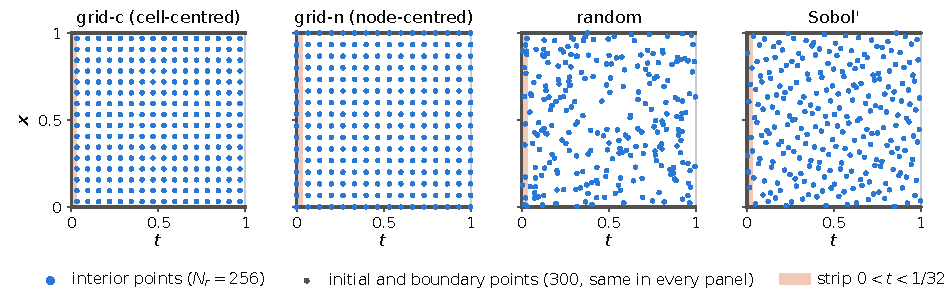
\includegraphics[width=\textwidth]{s3_methods_points.pdf}
\caption{The four fixed interior point sets for problem \PH\ on the space--time
square, $\Nr=256$: cell-centred and node-centred $16\times16$ grids, and the
\strat{random} and \strat{Sobol} sets of seed 0 as generated by the benchmark code. Grey
dots: the 300 initial and boundary points, the same in every panel. Shaded: the strip
$0<t<1/32$ between the initial line and the first column of the cell-centred grid. The
strategies \strat{resample} and \strat{RAD} change their sets during training
(Table~\ref{s3_methods:tab:samplers}) and are not shown.}
\label{s3_methods:fig:points}
\end{figure}
% src: code/s3_methods_points.py -> figures/s3_methods_points.pdf, data/s3_methods_points.json

Figure~\ref{s3_methods:fig:points} shows the four fixed sets for \PH. The cell-centred grid
leaves the strip $0<t<1/32$ next to the initial line without a residual point; the
node-centred grid has a column on the initial line but its next column is at $t=1/15$.

\subsection{Implementation of the low-dimensional runs}\label{S2:sec:impl}

% src: research_benchmark/results/runs/*.json (timing.lbfgs_batched_fevals / 1500 = 7.28, 2.51, 2.59, 2.15, 1.49, 1.84)
The multi-seed runs use our own L-BFGS for a stack of networks, with Armijo backtracking
(Section~\ref{sC_details:sec:settings}); a stack advances only when its slowest member has
accepted a step, and the stacks used between 1.5 and 7.3 evaluations per iteration, an
upper bound for each member. Section~\ref{sC_details:sec:validation} compares the two L-BFGS
implementations.

% src: research_benchmark/results/runs/*.json (timing.batch_size 25 or 50, device mps); research_benchmark/scripts/run_budget_sweep.py (specs: 3 samplers x 5 seeds = stacks of 15, device mps); data/s4_lowdim_gridcontrol.json (stacks: batch_size 40 and 20, device mps); data/s5_hard_laplace3d_smooth.json (note: run_batched on CPU, 5 seeds stacked; device cpu); notes/VERIFICATION.md (sec. 2.5, caveats 4 and 5); data/checks/machine_load.json; research_highdim/scripts/hd_core.py (torch.set_num_threads(1))
All low-dimensional experiments are run by one PyTorch package (\code{pinnbench}); the
benchmark trains 25 or 50 networks per stack, independent in exact arithmetic, stacked along
a batch axis on the GPU of an Apple-silicon machine (budget sweep of
Section~\ref{S3:sec:budget}: stacks of 15; control experiment of
Section~\ref{s4_lowdim:sec:strategy}: stacks of 40 and 20 on the GPU; \PLthreeS: 5 networks on
the CPU). The driver is validated against single-network training in
Section~\ref{sC_details:sec:validation}; in floating point the result of a network depends on
the size of its stack (Section~\ref{sC_details:sec:repro}). The $d$-dimensional runs use one
CPU thread. The machine, with 12 cores, was shared with other jobs throughout, which is why
Sections~\ref{s5_hard:sec} and~\ref{s6_highdim:sec} quote more than one time measurement
wherever a cost is stated.

\subsection{The penalty bias for \texorpdfstring{\Pone}{LapD} at \texorpdfstring{$d=2$}{d = 2}}

\begin{observation}[Size of the penalty bias for \Pone\ at $d=2$]\label{s3_methods:obs:robin}
% src: verify_research_highdim/results/v_robin_fd.json (rel_l2_N200; N100 vs N200 differ by <= 2.1e-4 relative)
% src: verify_research_highdim/scripts/v_robin_fd.py
For \Pone\ in dimension $d=2$, where $\uex=x_1x_2$ and $f=0$, the Robin problem of
Proposition~\ref{s3_methods:prop:robin}(a) was solved by second-order finite differences
(five-point scheme with ghost points; the solutions on grids of 100 and 200 cells per
side differ by less than 0.03 per cent in the quantity reported). The relative $L^2$
distance $\norm{\ubeta-\uex}/\norm{\uex}$ is $0.288$, $\sci{5.00}{-2}$,
$\sci{5.48}{-3}$ and $\sci{5.54}{-4}$ for $\bet=1$, $10$, $100$ and $1000$, that is,
between $0.50/\bet$ and $0.55/\bet$ for $\bet\ge10$, in line with part~(c); the bound of
part~(c) and the sharper bound of Corollary~\ref{s6_highdim:cor:bound}(b) are compared with these
values in Observation~\ref{sA_proofs:obs:sharp}, and the bias in dimension $d=3$ to $20$ is computed
in Observation~\ref{sA_proofs:obs:biasd} and, exactly, in Proposition~\ref{sA_proofs:prop:exact}.
% src: verify_research_highdim/results/v_summary.txt (rows 'robin'); notes/VERIFICATION.md (sec. 3.1, V5 and V9)
Deep Ritz networks trained with the protocol of Section~\ref{s3_methods:sec:highdim} (one
run for each $\bet$, 4000 iterations, with the verification code \textsf{V-dim} of
Section~\ref{s3_methods:sec:verif}) end at $\errL=0.290$ for $\bet=1$ and
$\sci{4.78}{-2}$ for $\bet=10$, that is, within 5 per cent of the bias of the Robin
minimiser and far from zero; at $\sci{1.02}{-2}$ for $\bet=100$, above the bias; and at
$\sci{5.89}{-2}$ for $\bet=1000$, about a hundred times the bias, where the error is that
of the optimisation. The distance of the networks from $\ubeta$ itself was not measured.
\end{observation}

% src: verify_research_highdim/results/v_summary.txt (robin, beta 10); verify_research_highdim/results/v_robin_fd.json (10: rel_l2_N200)
\noindent The bias is the error of the limit of the training, not a lower bound on the
error of a trained network: a network at distance $\norm{v-\ubeta}$ from the minimiser has
an error between $\norm{\ubeta-\uex}-\norm{v-\ubeta}$ and
$\norm{\ubeta-\uex}+\norm{v-\ubeta}$, and the run with $\bet=10$ indeed ends 4.5 per cent
below the bias. What a small $\bet$ does is to make training converge to a function that is
not the solution; in these runs a large $\bet$ in turn slowed the optimisation.
Section~\ref{s6_highdim:sec} returns to both effects. The proof of
Proposition~\ref{s3_methods:prop:robin}(a) also gives the identity
$\Eritz(v)-\Eritz(\ubeta)=\tfrac12\norm{\grad(v-\ubeta)}^2+\bet\,\nbd{v-\ubeta}^2$ quoted in
Section~\ref{s3_methods:sec:ritz}; the minimum of the loss is negative for \Ptwo\ and positive
for \Pone, where $f=0$.

\subsection{Two ways of computing the Laplacian}\label{S2:sec:lap}

The Laplacian in the PINN residual can be computed in two ways. Nested reverse-mode
differentiation takes one further backward pass for each of the $d$ coordinates.
Alternatively the triple $(u,\grad u,\lap u)$ can be propagated forward
through the layers~\citep{li2024forward}. Both are exact: at $d=2$ and $d=10$ the two
versions return the same single-precision loss value, digit for digit as printed (against
the separately written nested version of \textsf{V-dim} the single-precision losses agree
to seven or more significant digits up to $d=20$), and in double precision the Laplacians
differ by less than $10^{-16}$; they differ only in cost (Section~\ref{s6_highdim:sec:cost}).
The main runs of Section~\ref{s6_highdim:sec} use the forward version; five runs of the
weight sweep, made earlier, and \textsf{V-dim} use the nested one.
% src: research_highdim/results/check_core.txt (forward-vs-nested); verify_research_highdim/results/v_check.txt (V1); notes/VERIFICATION.md (sec. 3.1, V1 and V10; sec. 3.4); data/checks/study_records.json (highdim.sweep_runs_before_changes: five sweep runs with nested autograd)

% =====================================================================================
% sections/S3_lowdim.tex -- Supplementary Section S3: further results of the low-dimensional
% benchmark (Section 4).  Figures: code/s4_lowdim_figs.py, code/s4_lowdim_timeslices.py.
% The rows of Table s4_lowdim:tab:budget are written by code/s4_lowdim_tables.py.
% All `% src:` paths are relative to the root of the repository.
% =====================================================================================
\section{Low-dimensional benchmark: further results}\label{S3:sec}

\begin{figure}[tbp]
\centering
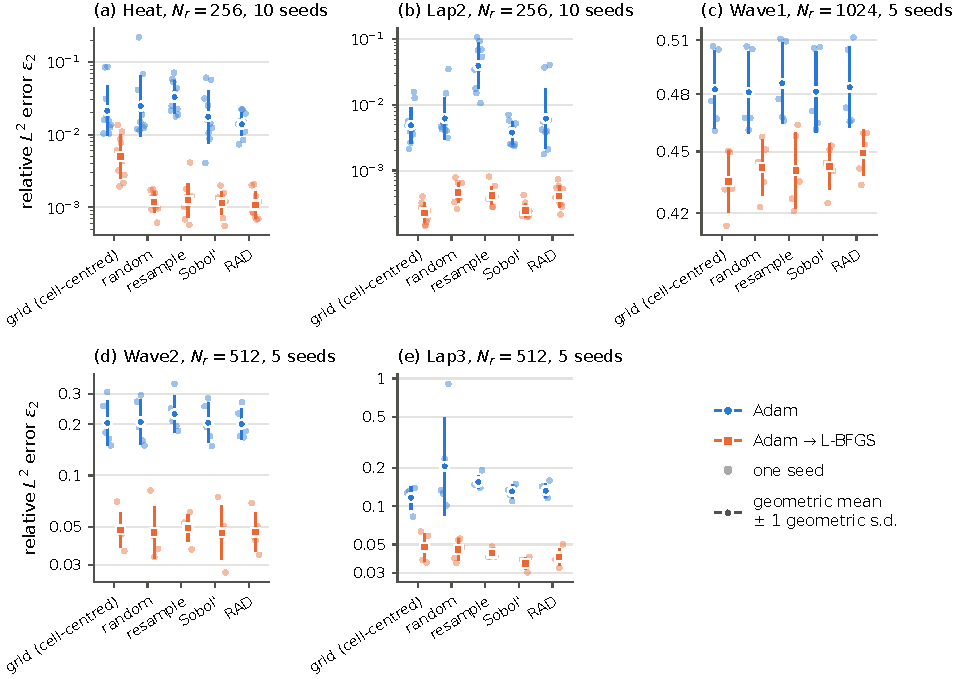
\includegraphics[width=\textwidth]{s4_lowdim_samplers.pdf}
\caption{Held-out relative $L^2$ error $\errL$ of every benchmark run, by problem and
collocation strategy, for the arms \Adam\ (blue circles, 3000 iterations) and \AdamLBFGS\
(orange squares, 1500 + 1500 iterations). Small dots: one seed each. Large markers with
bars: geometric mean over seeds and one geometric standard deviation either side.
``grid (cell-centred)'' is \strat{grid-c}. The evaluation sets are those of
Table~\ref{s2_problems:tab:problems}; the vertical scales differ between panels.}
\label{s4_lowdim:fig:samplers}
\end{figure}
% src: research_benchmark/results/runs/*_s*-*.json -> code/s4_lowdim_figs.py samplers

\subsection{Optimiser}\label{S3:sec:optimiser}

\begin{figure}[tbp]
\centering
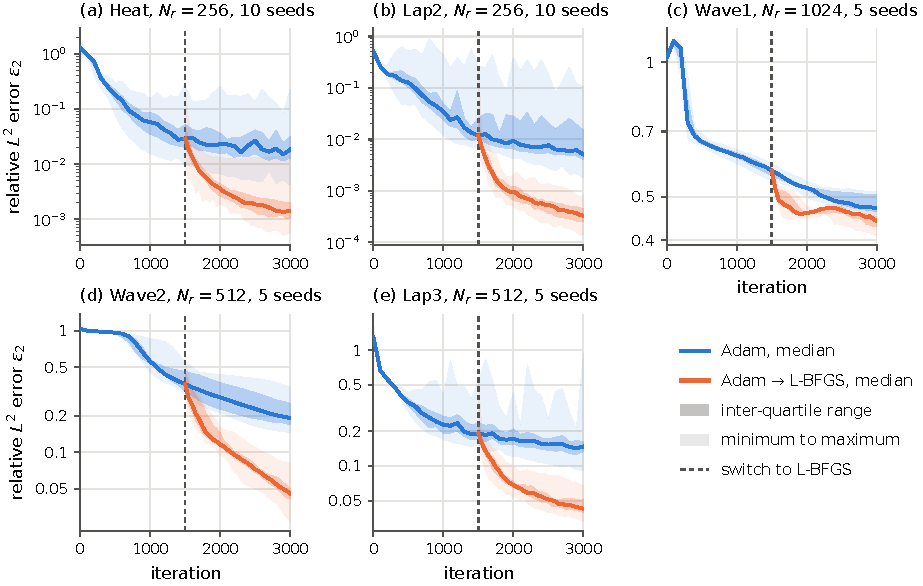
\includegraphics[width=\textwidth]{s4_lowdim_curves.pdf}
\caption{Relative $L^2$ error during training for the arms \Adam\ (blue) and \AdamLBFGS\
(orange), measured every 100 \Adam\ iterations and every 50 \LBFGS\ iterations on a fixed
random subset of 4096 points of the held-out evaluation set. Line: median over all
strategies and seeds (50 runs per arm for \PH\ and \PLtwo, 25 for \PWone, \PWtwo\ and
\PLthree); dark band: inter-quartile range; light band: minimum to maximum. Dashed line:
iteration 1500, where the \AdamLBFGS\ arm branches from the \Adam\ run.}
\label{s4_lowdim:fig:curves}
\end{figure}
% src: research_benchmark/results/runs/*_s*-*.json (curve.test_rel_l2) -> code/s4_lowdim_figs.py curves; research_benchmark/pinnbench/problems.py (test_subset, n = 4096); research_benchmark/pinnbench/core.py (log_every = 100, callback_every = 50)

% src: verify_research_benchmark/v_summary.out ("L-BFGS arm better than Adam arm in 39 of 40 of the re-check runs"; heat1d|grid|1: 1.303e-02 | 1.316e-02 against 1.582e-02 | 1.359e-02 in the benchmark)
% src: data/s4_lowdim_numbers.json (optimiser.*.closest_pair_ratio_lbfgs_over_adam: heat1d 0.859, laplace2d 0.244, wave2d 0.314, laplace3d 0.547, wave1d 0.995)
In \textsf{V-bench} the \AdamLBFGS\ arm is the better one in 39 of 40 pairs; the exception
is \PH\ with \strat{grid-c} and seed~1 ($\sci{1.303}{-2}$ for \Adam\ against
$\sci{1.316}{-2}$). The same network is the closest pair of the benchmark on \PH\
($\sci{1.58}{-2}$ against $\sci{1.36}{-2}$, a ratio of 0.86) and, \PWone\ apart, where
neither arm succeeds and the closest pair has the ratio 0.995, of the whole benchmark.
% src: data/s4_lowdim_numbers.json (adam_fluctuation_max_over_min_it1500_3000), computed by code/s4_lowdim_tables.py from research_benchmark/results/runs/*_s*-*.json
The logged \Adam\ errors of one run fluctuate by a median factor of 8.0 on \PH\ (largest factor
41) and of 28 on \PLtwo\ (largest 246) between iterations 1500 and 3000
(Figure~\ref{s4_lowdim:fig:curves}).

% src: verify_research_benchmark/v_adam_decay.json; data/s4_lowdim_numbers.json (replication: adam_exponential_decay, adam_constant_lr_same_runs, adam_decay_over_constant_same_runs: heat 1.00, 0.85, 0.22; laplace2d 2.30, 4.39, 5.28)
One alternative to the constant learning rate of the \Adam\ arm was tried, in
\textsf{V-bench} with \strat{random} points and seeds 0 to 2: a rate that decays
exponentially from $10^{-3}$ to $10^{-5}$ over the 3000 iterations. Compared with the
constant-rate runs of the same code and seeds, it ended at $\sci{3.1}{-2}$, $\sci{2.3}{-2}$
and $\sci{2.0}{-2}$ against $\sci{3.1}{-2}$, $\sci{2.7}{-2}$ and $\sci{9.3}{-2}$ on \PH, and
at $\sci{1.7}{-2}$, $\sci{2.0}{-2}$ and $\sci{2.3}{-2}$ against $\sci{7.4}{-3}$,
$\sci{4.6}{-3}$ and $\sci{4.4}{-3}$ on \PLtwo. On \PH\ this schedule ended at 1.00,
0.85 and 0.22 times the constant-rate error, which is still more than ten times the
error of the \AdamLBFGS\ arm; on \PLtwo\ it was 2.3 to 5.3 times worse. It did not close
the gap; it is not a tuned \Adam\ baseline.

\subsection{Collocation strategy}\label{S3:sec:strategy}

\begin{figure}[tbp]
\centering
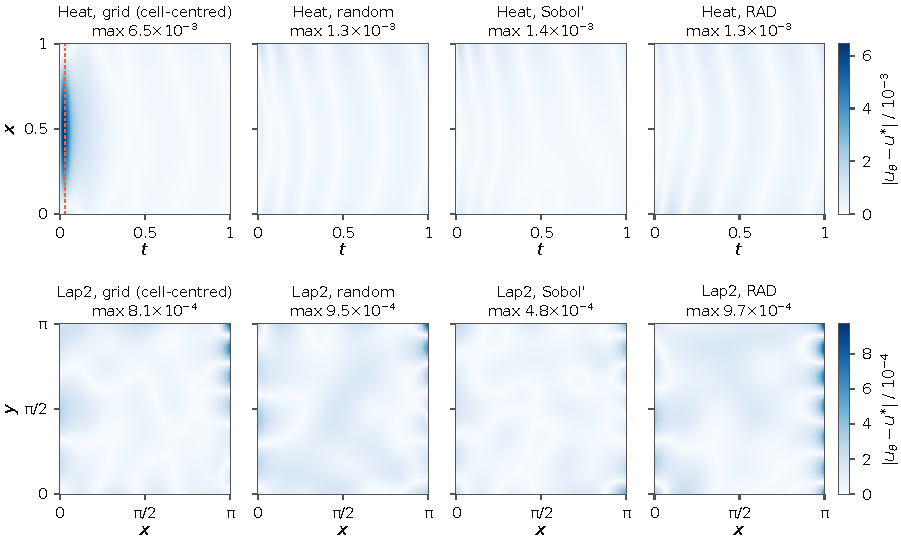
\includegraphics[width=\textwidth]{s4_lowdim_errmaps.pdf}
\caption{Pointwise absolute error $\abs{\unet-\uex}$ on the $201\times201$ evaluation
grid for seed~0 after \AdamLBFGS, with $\Nr=256$. Top row: \PH\ (time horizontal);
bottom row: \PLtwo. Columns: \strat{grid-c}, \strat{random}, \strat{Sobol}, \strat{RAD}.
Each row has one linear colour scale, in units of $10^{-3}$ and $10^{-4}$. The dashed
line in the first panel is $t=1/32$, the first column of the cell-centred grid. One seed
is shown; the statistics are in Tables~\ref{s4_lowdim:tab:strategy}
and~\ref{s4_lowdim:tab:gridcontrol}.}
\label{s4_lowdim:fig:errmaps}
\end{figure}
% src: research_benchmark/results/runs/heat1d_pred_seed0.npz, laplace2d_pred_seed0.npz -> code/s4_lowdim_figs.py errmaps

% src: data/s4_lowdim_errmaps_info.json (computed by code/s4_lowdim_figs.py from research_benchmark/results/runs/heat1d_pred_seed0.npz)
In the error field of seed~0 (Figure~\ref{s4_lowdim:fig:errmaps}) the largest error of
\strat{grid-c} on \PH, $\sci{6.5}{-3}$, is at $t=0.025$.
% src: data/s4_lowdim_gridcontrol.json (strategies.*.adam_lbfgs.share_sq_error_t_le_0.05)
In the control experiment of Section~\ref{s4_lowdim:sec:strategy}, in 9 of 10 seeds between
67 and 73 per cent of the squared error of \strat{grid-c} lies in $t\le0.05$, against a median
of 25 per cent for \strat{random} (Table~\ref{s4_lowdim:tab:gridcontrol}).
% src: data/s4_lowdim_gridcontrol.json (vs_random.adam_lbfgs: gridn per seed 1.16 1.50 5.33 1.05 1.25 0.52 5.96 0.94 7.21 3.65); verify_research_benchmark/v_summary.out ("cell-grid/random geo ratio 3.94 ... 0/6 p=0.031"; "node-grid/random 1.26 per-seed [1.08, 1.13, 5.2, 0.95, 1.27, 0.52] better 2/6 p=0.438"; "node-grid/cell-grid 0.32 ... 5/6 p=0.094"); verify_research_benchmark/v_runs.json; verify_research_benchmark/v_runs_extra.json
The per-seed ratios of the node-centred grid \strat{grid-n} to \strat{random} in the control
range from 0.52 to 7.2. In \textsf{V-bench}, with 6 seeds, \strat{grid-n} was 1.26 times
\strat{random} (per-seed ratios 1.08, 1.13, 5.2, 0.95, 1.27 and 0.52; $p=0.44$) and 0.32
times \strat{grid-c}, while the same code reproduced the penalty of \strat{grid-c}, 3.94
times \strat{random} (worse in 6 of 6). It is not established that a grid with a column on
the initial line loses all of the penalty. On \PLtwo\ the grid result concerns the
cell-centred grid; \strat{grid-n} was not run there.

% src: research_benchmark/pinnbench/samplers.py (RADSampler: period = 500, pool_factor = 8; for_lbfgs: one update); research_benchmark/pinnbench/core.py (run_batched: "it % rad_period == 0 and it < n_adam"; one update at the branch point)
% src: refs.bib (wu2023, annote: arXiv:2207.10289, Sec. 3.3: "first trained using 15,000 steps of Adam and then 1,000 steps of L-BFGS ... resampled every 2,000 iterations (1,000 iterations using Adam followed by 1,000 iterations using L-BFGS)"; read 2026-10-01)
\paragraph{The adaptive strategy.} In the \AdamLBFGS\ arm the set of \strat{RAD} is the
\strat{Sobol} set for the first 500 iterations and is then redrawn four times only, from
a pool of $8\Nr$ points: at iterations 500, 1000 and 1500 and once more before \LBFGS,
the third set serving a single iteration. It is fixed during the 1500 \LBFGS\ iterations,
in which most of the error is removed. \citet{wu2023}, in their Burgers example, first
train for 16\,000 iterations and then redraw every 2000 iterations, half of which are
\LBFGS\ iterations. On \PLthree, the one problem whose solution is not smooth and on which a
residual-adaptive strategy would be expected to matter most, \strat{RAD} has the ratio 0.88
to \strat{random}, better in 3 of 5 seeds.
% src: research_benchmark/results/tables.md (T3)

\paragraph{Sobol' points seed by seed.}
% src: research_benchmark/results/tables.md (T3); verify_research_benchmark/v_stats.out (heat1d adam_lbfgs sobol per-seed ratios: 1.18, 1.12, 1.45, 1.25 above 1)
The ratios of \strat{Sobol} to \strat{random} after \AdamLBFGS\ are 0.97, 0.54, 1.00, 0.99 and
0.78 for \PH, \PLtwo, \PWone, \PWtwo\ and \PLthree; on \PH\ four of the ten per-seed ratios
are above 1 (1.18, 1.12, 1.45 and 1.25), and on \PLthree\ \strat{Sobol} is better in 5 of 5
seeds, which five seeds cannot make significant.

% src: data/s4_lowdim_numbers.json (replication.lap2d_lbfgs_resample_over_random_3seeds: ratio 1.56, per seed 2.15, 1.90, 0.94), from verify_research_benchmark/v_runs.json
\paragraph{Resampling after \LBFGS.} The three \textsf{V-bench} seeds on \PLtwo\ give the
ratio 1.56 of \strat{resample} to \strat{random} after \AdamLBFGS\ (per seed 2.15, 1.90 and
0.94; better in 1 of 3 seeds).

\subsection{Point budget}\label{S3:sec:budget}

\begin{table}[tbp]
\centering
\caption{Budget sweep on problem \PH, arm \AdamLBFGS, seeds 0 to 4: mean $\pm$
sample standard deviation of $\errL$, and the ratio to \strat{random} with the same seed
(geometric mean; in brackets the number of seeds in which the strategy is better and the
exact two-sided Wilcoxon $p$-value, whose smallest attainable value is 0.0625). The row
$\Nr=256$ is the benchmark, restricted to the same five seeds.}
\label{s4_lowdim:tab:budget}
% src: research_benchmark/results/budget_sweep.json; research_benchmark/results/tables.md (T6); paired ratios and p-values: data/s4_lowdim_numbers.json (budget), agreeing with verify_research_benchmark/v_json.out (budget sweep: grid/random 2.02, p=0.312; sobol/random 0.41, p=0.438)
\footnotesize
\setlength{\tabcolsep}{4pt}
\begin{tabular}{@{}rccccc@{}}
\toprule
 & \multicolumn{3}{c}{$\errL$, mean $\pm$ s.d.} & \multicolumn{2}{c}{ratio to \strat{random}} \\
\cmidrule(lr){2-4}\cmidrule(l){5-6}
$\Nr$ & \strat{grid-c} & \strat{random} & \strat{Sobol} & \strat{grid-c} & \strat{Sobol} \\
\midrule
%% BEGIN GENERATED s4_lowdim:tab:budget
64 & $(7.21\pm3.09)\times10^{-2}$ & $(4.76\pm4.45)\times10^{-2}$ & $(1.64\pm1.27)\times10^{-2}$ & 2.02 (1/5; 0.312) & 0.41 (3/5; 0.438) \\
256 & $(6.71\pm4.67)\times10^{-3}$ & $(1.45\pm0.34)\times10^{-3}$ & $(1.35\pm0.37)\times10^{-3}$ & 3.79 (0/5; 0.0625) & 0.93 (3/5; 0.438) \\
1024 & $(1.23\pm0.45)\times10^{-3}$ & $(1.13\pm0.43)\times10^{-3}$ & $(1.15\pm0.41)\times10^{-3}$ & 1.11 (1/5; 0.438) & 1.02 (2/5; 0.812) \\
%% END GENERATED s4_lowdim:tab:budget
\bottomrule
\end{tabular}
\end{table}

\begin{figure}[tbp]
\centering
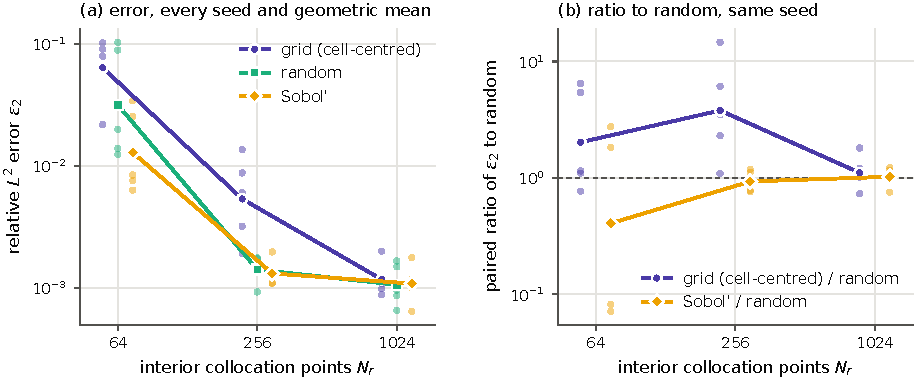
\includegraphics[width=\textwidth]{s4_lowdim_budget.pdf}
\caption{Budget sweep on problem \PH, arm \AdamLBFGS, seeds 0 to 4.
(a)~Relative $L^2$ error $\errL$ against the number $\Nr$ of interior points for
\strat{grid-c}, \strat{random} and \strat{Sobol}; dots: single seeds, lines: geometric
means. (b)~Ratio of $\errL$ to that of \strat{random} with the same seed; lines: geometric
mean of the ratios. Markers are displaced horizontally for legibility; the budgets are
64, 256 and 1024.}
\label{s4_lowdim:fig:budget}
\end{figure}
% src: research_benchmark/results/budget_sweep.json -> code/s4_lowdim_figs.py budget

With 64 points neither paired difference is distinguishable from none
(Table~\ref{s4_lowdim:tab:budget}).
% src: verify_research_benchmark/v_summary.out ("heat N=1024: grid 0.0011, 0.00082; random 0.00129, 0.00081"); verify_research_benchmark/v_runs_budget.json
\textsf{V-bench} confirms the agreement at 1024 points on two seeds (\strat{grid-c}
$\sci{1.10}{-3}$ and $\sci{8.2}{-4}$; \strat{random} $\sci{1.29}{-3}$ and $\sci{8.1}{-4}$).
We do not extend the conclusion of the sweep to the other problems or to larger budgets.

\subsection{Error on time slices}\label{S3:sec:timeslice}

% src: data/s4_lowdim_timeslices.json (summary); rows generated by code/s4_lowdim_timeslices.py merge -> data/s4_lowdim_timeslices_table.tex
\begin{table}[tbp]
\centering
\caption{Problem \PH, $\Nr=256$, 10 seeds: relative $L^2$ error in per cent on the
whole evaluation grid ($\errL$) and on single time slices ($\errT(t)$); geometric means
over seeds, and the range over seeds at $t=1$. Figure~\ref{s4_lowdim:fig:timeslice} shows
every run.}
\label{s4_lowdim:tab:timeslice}
\footnotesize
\setlength{\tabcolsep}{4.5pt}
\begin{tabular}{@{}llrrrrrrrr@{}}
\toprule
 & & & \multicolumn{6}{c}{$100\,\errT(t)$ at $t=$} & range at \\
\cmidrule(lr){4-9}
strategy & arm & $100\,\errL$ & 0 & 0.1 & 0.25 & 0.5 & 0.75 & 1 & $t=1$ \\
\midrule
%% BEGIN GENERATED s4_lowdim:tab:timeslice
\strat{random} & \Adam & 1.58 & 0.572 & 1.09 & 3.82 & 24.9 & 420 & 5849 & 2360--52\,582 \\
\strat{random} & \AdamLBFGS & 0.107 & 0.0436 & 0.0777 & 0.235 & 2.26 & 20.9 & 479 & 156--1241 \\
\strat{Sobol} & \Adam & 2.06 & 0.625 & 1.50 & 5.36 & 41.2 & 536 & 7242 & 1965--107\,521 \\
\strat{Sobol} & \AdamLBFGS & 0.116 & 0.0421 & 0.0886 & 0.349 & 3.49 & 32.6 & 567 & 198--1298 \\
%% END GENERATED s4_lowdim:tab:timeslice
\bottomrule
\end{tabular}
\end{table}



% src: data/s4_lowdim_timeslices.json (share_of_sq_error.t_le_0.25: medians 0.42 to 0.64 over the four cells, 0.08 to 0.91 over the 40 runs; runs[*].adam_lbfgs.lbfgs_iters)
The error itself is not concentrated at early times: in these runs the time levels
$t\le0.25$ carry 42 to 64 per cent of the squared error (medians of the four combinations of
strategy and arm). Six of the 20 \LBFGS\ phases stopped on the tolerance of the PyTorch
optimiser after 1365 to 1493 of their 1500 iterations.

% =====================================================================================
% sections/S4_hard.tex -- Supplementary Section S4: further results on the harder problems and
% the classical baselines (Section 5).
% All `% src:` paths are relative to the root of the repository.
% =====================================================================================
\section{Harder problems and classical baselines: further results}\label{S4:sec}

\subsection{Longer runs on \texorpdfstring{\PWtwo}{Wave2}}\label{S4:sec:w2}

% src: data/s5_hard_wave2d_long.json (adam_lbfgs_test_rel_l2_at 3000: 7.44e-2, 4.54e-2, 4.50e-2); research_benchmark/results/runs/wave2d_s0-5.json (sobol, seeds 0-2, adam_lbfgs curve at iteration 3000, test_rel_l2: 7.28e-2, 4.58e-2, 4.36e-2; the full-grid values in benchmark_runs.csv are 7.47e-2, 4.61e-2, 4.41e-2)
At iteration 3000 the longer runs of Section~\ref{s5_hard:sec:w2} agree with the benchmark
runs of the same seeds ($\sci{7.4}{-2}$, $\sci{4.5}{-2}$, $\sci{4.5}{-2}$ against
$\sci{7.3}{-2}$, $\sci{4.6}{-2}$, $\sci{4.4}{-2}$, both on the 4096-point subset of the
evaluation grid on which the training curves are logged). The \LBFGS\ phase stops on the
termination test of the optimiser (gradient below $10^{-9}$, or step or loss change below
$10^{-12}$).
% src: data/s5_hard_wave2d_long.json (adam_lbfgs_test_ratio_3000_over_2000, adam_lbfgs_test_ratio_9500_over_8500); research_benchmark/pinnbench/core.py (run_single: tolerance_grad, tolerance_change)
Between iterations 2000 and 3000 the error falls by a factor of 2.1 to 3.3; over the last
1000 logged iterations before iteration 9500 it still falls by 8 to 15 per cent
(Figure~\ref{s5_hard:fig:wave2d}).

\begin{figure}[tbp]
\centering
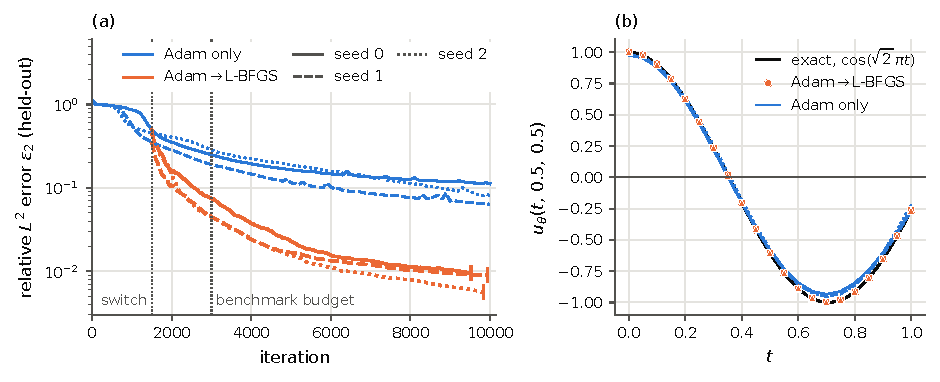
\includegraphics[width=\textwidth]{s5_hard_wave2d.pdf}
\caption{Problem \PWtwo, \strat{Sobol} points, $\Nr=512$, seeds 0, 1, 2 (longer runs of
Section~\ref{s5_hard:sec:w2}).
(a) Relative $L^2$ error on a fixed random subset of 4096 points of the
$21\times81\times81$ held-out grid against the iteration number, for 10\,000 \Adam\
iterations (blue) and for 1500 \Adam\ iterations followed by \LBFGS\ (orange); the dotted
vertical lines mark the switch and the 3000-iteration budget of the benchmark, and the
short vertical ticks the iteration at which \LBFGS\ stopped. (b) Value of the trained
networks at the point $(x,y)=(0.5,0.5)$ at $t=0,0.05,\dots,1$: markers, \AdamLBFGS\ (three
seeds, one marker shape each); blue lines, \Adam\ only; black line, exact solution.}
\label{s5_hard:fig:wave2d}
% src: code/s5_hard_wave2d_long.py (plot); data/s5_hard_wave2d_long.json
\end{figure}

\subsection{The two modes of \texorpdfstring{\PWone}{Wave1}}\label{S4:sec:w1}

% src: data/s5_hard_wave1d_long.json (summary.benchmark_seed0: rel_l2_a1 0.078 to 0.117 (Adam), 0.036 to 0.092 (Adam -> L-BFGS); rms_a4_over_rms_exact 0.060 to 0.064 and 0.226 to 0.250; share_sq_error_mode4 0.89 to 0.93 and 0.84 to 0.89), computed by code/s5_hard_wave1d_long.py from research_benchmark/results/runs/wave1d_pred_seed0.npz
We projected the ten stored predictions of seed 0 of the benchmark (five strategies, two
arms) onto the two spatial modes,
$a_k(t)=\ip{\unet(t,\cdot)}{\sin k\pi x}/\ip{\sin k\pi x}{\sin k\pi x}$ for $k=1,4$. The
amplitude of the slow mode is reproduced to 8 to 12 per cent after \Adam\ and 4 to 9 per
cent after \AdamLBFGS\ (relative $L^2$ error of $a_1$ over $t$); the amplitude of the fast
mode has a root-mean-square value of 6 per cent of the exact one after \Adam\ and 23 to 25
per cent after \AdamLBFGS, and the fast mode carries 84 to 93 per cent of the squared error.
% src: data/s5_hard_wave1d_long.json (adam_lbfgs_test_rel_l2_at 3000); research_benchmark/results/runs/wave1d_s0-5.json (sobol, seeds 0-2, adam_lbfgs curve at iteration 3000: 0.4416, 0.4187, 0.4479)
At iteration 3000 the longer runs of Section~\ref{s5_hard:sec:w1} agree with the benchmark
runs of the same seeds (0.442, 0.414 and 0.452 against 0.442, 0.419 and 0.448, both on the
4096-point subset on which the curves are logged).
% src: data/s5_hard_wave1d_long.json (summary.per_seed[*].adam_lbfgs_modes and adam_modes: rms_a4_over_rms_exact 0.35 to 0.43)
In the six longer runs the root-mean-square amplitude of the fast mode is 0.35 to 0.43 of the
exact one.

\begin{figure}[tbp]
\centering
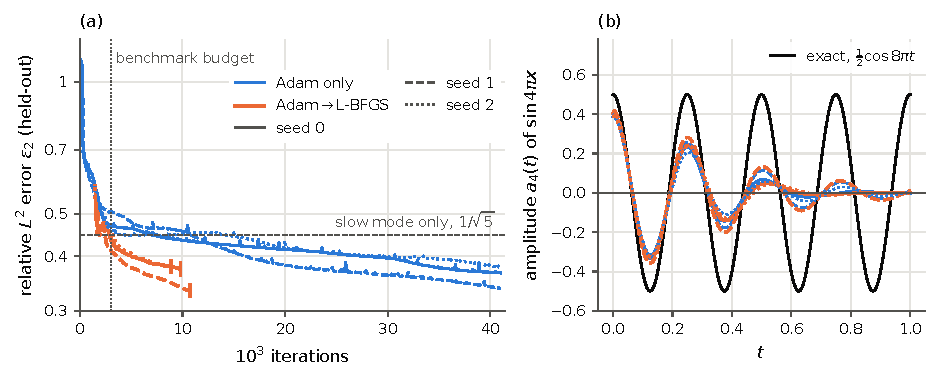
\includegraphics[width=\textwidth]{s5_hard_wave1d.pdf}
\caption{Problem \PWone, \strat{Sobol} points, $\Nr=1024$, seeds 0, 1, 2 (longer runs of
Section~\ref{s5_hard:sec:w1}).
(a)~Relative $L^2$ error on a fixed random subset of 4096 points of the $201\times201$
held-out grid against the iteration number, for 41\,000 \Adam\ iterations (blue) and for
1500 \Adam\ iterations followed by \LBFGS\ (orange); the short vertical ticks mark the
iteration at which \LBFGS\ stopped, the dotted vertical line the budget of the benchmark,
and the dashed horizontal line the error $1/\sqrt5$ of a predictor that contains the slow
mode only. (b)~Amplitude $a_4(t)$ of the fast mode $\sin4\pi x$ in the trained networks
(same colours and line styles), against the exact amplitude $\tfrac12\cos8\pi t$ (black).}
\label{s5_hard:fig:wave1d}
% src: code/s5_hard_wave1d_long.py (plot); data/s5_hard_wave1d_long.json
\end{figure}

\subsection{Finite differences}\label{S4:sec:fd}

% src: research_benchmark/results/classical.csv (observed_order_rel_l2); research_benchmark/pinnbench/classical.py (evaluate)
% src: data/s5_hard_fd_lap3s.json (Lap3s: rel_l2 2.105e-3, 5.286e-4, 1.323e-4, 3.307e-5 for n = 20, 40, 80, 160; observed orders 1.994, 1.999, 2.000; Lap3: 1.968, 2.698, 1.894), script code/s5_hard_fd_lap3s.py
On \PLthree\ the observed order of the seven-point scheme is 1.97, 2.70 and 1.89
(Table~\ref{sC_details:tab:fdconv}): the value 2.70 occurs where the evaluation changes from
cubic interpolation ($n=20,40$) to nodal values ($n=80,160$) of the cell-centred evaluation
grid, and the last value, between two nodal evaluations, is somewhat below two. The datum on
the face $x=\pi$ is the cause of both irregularities: with the compatible single-mode datum
of \PLthreeS\ the same solver and the same evaluation give $\errL=\sci{2.11}{-3}$,
$\sci{5.29}{-4}$, $\sci{1.32}{-4}$ and $\sci{3.31}{-5}$ for $n=20$, 40, 80 and 160, that is,
the orders 1.99, 2.00 and 2.00. Since \PLthreeS\ also makes the solution a single mode, the
comparison does not separate the compatibility of the data from the modal content; that the
discontinuity is what lowers the order is what the theory of the scheme leads one to expect,
since the scheme is of second order for smooth solutions.
% src: verify_research_benchmark/v_fd.out (heat1d n=100, laplace2d n=100, wave2d n=20, laplace3d n=20, 40; extracted by code/s5_hard_tables.py, info.n_runs_B.*.rederived_rel_l2); notes/VERIFICATION.md (sec. 2.1; sec. 2.3, item 7)
The finite-difference errors do not rest on one code: the verification re-derived them from
closed-form solutions of the discrete schemes and from a separate sparse solve. For the grids
of Table~\ref{s5_hard:tab:fd} it obtained $\sci{4.918}{-4}$ for \PH\ (on the nodes of the
finite-difference grid, not on the interpolated evaluation grid), $\sci{7.508}{-5}$ for
\PLtwo, $\sci{5.121}{-3}$ for \PWtwo\ and $\sci{9.968}{-3}$ for \PLthree\ ($\sci{3.900}{-2}$
for $n=20$); \PWone\ was not re-derived.

\subsection{Cost}\label{S4:sec:cost}

% src: research_benchmark/results/timing_single.json; research_benchmark/scripts/time_single.py
(A)~The single-network driver was timed for 400 \Adam\ and 200 \LBFGS\ iterations while the
load average was 95 to 167 and extrapolated to 3000 iterations.
% src: verify_research_benchmark/v_runs.json; verify_research_benchmark/v_runs_extra.json; verify_research_benchmark/v_summary.out (t_arm); data/checks/machine_load.json (lowdim_verification_runs_B: load about 20 to 45); data/sC_details_numbers.json (verifier_lowdim.B: n_stopped_early = 12, min_lbfgs_iters = 1178)
(B)~The runs of \textsf{V-bench} comprise 21 runs for \PH, 12 for \PLtwo\ and one for each
other problem. Twelve of these 36 runs, all on \PH\ and \PLtwo, stopped on the tolerance of
\LBFGS\ after 1178 or more of its 1500 iterations, which makes the lower ends of the ranges,
if anything, too low.
% src: research_benchmark/results/runs/*_s*-*.json (timing: (t_adam_to_branch + t_lbfgs_total) / batch_size = 12.4 s (heat1d, 50 networks), 11.5 and 13.9 s (laplace2d, two stacks of 25), 6.9 s (wave1d), 7.4 s (wave2d), 11.7 s (laplace3d)); data/s5_hard_cost.json (time_C_stacked_gpu_per_network_s)
(C)~The training time of the \AdamLBFGS\ arm of a stack divided by the number of networks in
it is 12.4~s for \PH\ (50 networks), 11.5 and 13.9~s for \PLtwo\ (two stacks of 25), 6.9~s
for \PWone, 7.4~s for \PWtwo\ and 11.7~s for \PLthree; the load during these runs was not
recorded. Table~\ref{sC_details:tab:cost} keeps the three measurements apart.

\begin{figure}[tbp]
\centering
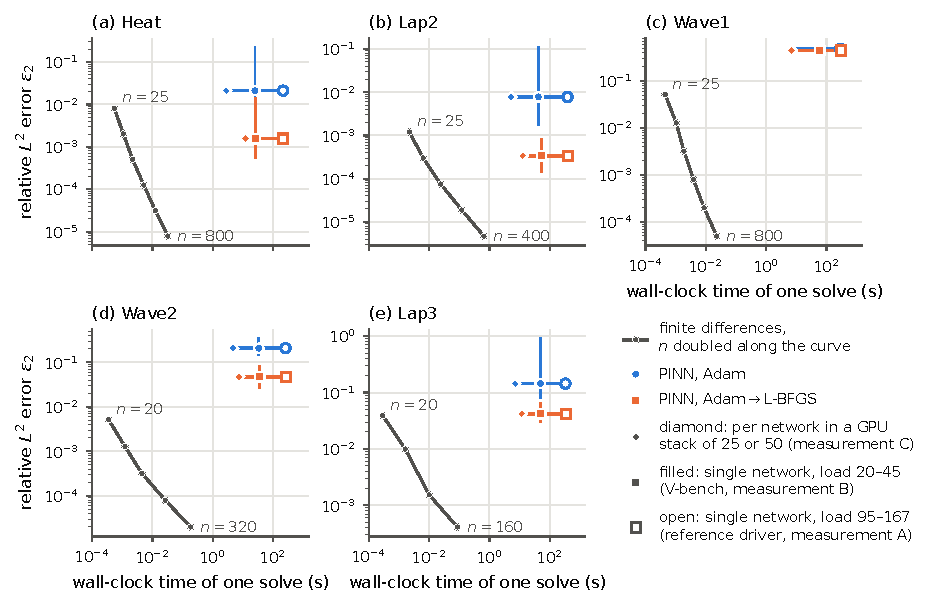
\includegraphics[width=\textwidth]{s5_hard_cost.pdf}
\caption{Accuracy against wall-clock time of one solve, one panel per problem. Grey:
second-order finite differences, the grid parameter $n$ doubling along each curve (time:
best of three solves). Blue circles and orange squares: \Adam\ and \AdamLBFGS\ arms of the
benchmark (3000 iterations); the ordinate is the geometric mean of $\errL$ over all
strategies and seeds (50 runs for \PH\ and \PLtwo, 25 otherwise) and the vertical bar its
range over those runs. Each PINN arm is drawn at three times, the measurements C, B and A
of Section~\ref{s5_hard:sec:fd}: diamond, time per network in the GPU stacks of the
benchmark; filled marker, median of the single-network runs of \textsf{V-bench}; open
marker, single-network driver under heavy load. The horizontal bar spans the three. All
errors are on the held-out sets of Table~\ref{s2_problems:tab:problems}.}
\label{s5_hard:fig:cost}
% src: code/s5_hard_cost.py; data/s5_hard_cost.json
\end{figure}

% =====================================================================================
% sections/S5_highdim.tex -- Supplementary Section S5: further results of the dimension study
% (Section 6).  Table rows between GENERATED markers are written by code/s6_highdim_tables.py,
% code/s6_highdim_bound.py and code/s6_highdim_remedies.py (code/inject.py finds the marker in
% any section file).  All `% src:` paths are relative to the root of the repository.
% =====================================================================================
\section{Dimension study: further results}\label{S5:sec}

\subsection{Errors at equal iterations, verification runs and training curves}\label{S5:sec:vdim}

\begin{table}[tbp]
\centering
\caption{Problem \Pone\ after 4000 iterations, three seeds: errors on the 50\,000 held-out
points in units of $10^{-2}$ (so $1.260$ means $\sci{1.260}{-2}$). For $\errL$: mean
$\pm$ sample standard deviation, with [minimum, maximum] underneath; for $\errH$ and the
centred error $\errC$: means. Ratio: mean $\errL$ of Deep Ritz divided by that of the
PINN. Floors: $\errL$ of the best affine and of the best constant approximation of $\uex$
(Proposition~\ref{s2_problems:prop:floors}).}
\label{s6_highdim:tab:p1}
\small
\setlength{\tabcolsep}{4.5pt}
% src: research_highdim/results/runs.csv (phase main), research_highdim/results/summary.csv; floors: data/closed_forms.json
% generated by code/s6_highdim_tables.py -> data/s6_highdim_tables.tex
\begin{tabular}{@{}r cc c cc cc cc@{}}
\toprule
 & \multicolumn{2}{c}{$\errL$} & & \multicolumn{2}{c}{$\errH$} & \multicolumn{2}{c}{$\errC$} & \multicolumn{2}{c}{floor of $\errL$}\\
\cmidrule(lr){2-3}\cmidrule(lr){5-6}\cmidrule(lr){7-8}\cmidrule(l){9-10}
$d$ & PINN & Deep Ritz & ratio & PINN & Deep Ritz & PINN & Deep Ritz & affine & constant\\
\midrule
2 & $0.608\pm0.187$ & $1.882\pm0.347$ & 3.10 & 2.14 & 6.05 & 0.92 & 2.85 & 25.0 & 66.1 \\
 & {\footnotesize $[0.392,\,0.721]$} & {\footnotesize $[1.527,\,2.220]$} &  &  &  &  &  &  &  \\[2pt]
3 & $0.672\pm0.255$ & $1.421\pm0.337$ & 2.11 & 2.40 & 5.43 & 1.01 & 2.14 & 25.0 & 66.1 \\
 & {\footnotesize $[0.457,\,0.954]$} & {\footnotesize $[1.160,\,1.802]$} &  &  &  &  &  &  &  \\[2pt]
5 & $0.760\pm0.055$ & $1.113\pm0.077$ & 1.46 & 3.29 & 5.05 & 1.44 & 2.11 & 20.0 & 52.9 \\
 & {\footnotesize $[0.698,\,0.804]$} & {\footnotesize $[1.039,\,1.192]$} &  &  &  &  &  &  &  \\[2pt]
10 & $1.260\pm0.084$ & $1.896\pm0.159$ & 1.50 & 6.45 & 9.63 & 3.42 & 5.15 & 13.9 & 36.7 \\
 & {\footnotesize $[1.171,\,1.337]$} & {\footnotesize $[1.730,\,2.047]$} &  &  &  &  &  &  &  \\[2pt]
20 & $4.663\pm0.248$ & $4.613\pm0.178$ & 0.99 & 24.51 & 26.71 & 17.30 & 17.11 & 10.2 & 26.9 \\
 & {\footnotesize $[4.381,\,4.848]$} & {\footnotesize $[4.416,\,4.764]$} &  &  &  &  &  &  &  \\
\bottomrule
\end{tabular}
\end{table}

\begin{table}[tbp]
\centering
\caption{Problem \Ptwo\ after 4000 iterations, three seeds; quantities and units as in
Table~\ref{s6_highdim:tab:p1}. Here $\errC=\errL$ because $\uex$ has zero mean, and the
best constant has $\errL=1$.}
\label{s6_highdim:tab:p2}
\small
\setlength{\tabcolsep}{6pt}
% src: research_highdim/results/runs.csv (phase main), research_highdim/results/summary.csv; floors: data/closed_forms.json
% generated by code/s6_highdim_tables.py -> data/s6_highdim_tables.tex
\begin{tabular}{@{}r cc c cc c@{}}
\toprule
 & \multicolumn{2}{c}{$\errL$} & & \multicolumn{2}{c}{$\errH$} & floor of $\errL$\\
\cmidrule(lr){2-3}\cmidrule(lr){5-6}\cmidrule(l){7-7}
$d$ & PINN & Deep Ritz & ratio & PINN & Deep Ritz & affine\\
\midrule
2 & $0.134\pm0.049$ & $0.574\pm0.121$ & 4.29 & 0.73 & 2.70 & 12.0 \\
 & {\footnotesize $[0.102,\,0.190]$} & {\footnotesize $[0.441,\,0.678]$} &  &  &  &  \\[2pt]
3 & $0.380\pm0.038$ & $1.426\pm0.183$ & 3.76 & 1.82 & 5.83 & 12.0 \\
 & {\footnotesize $[0.347,\,0.421]$} & {\footnotesize $[1.215,\,1.536]$} &  &  &  &  \\[2pt]
5 & $0.929\pm0.053$ & $1.509\pm0.041$ & 1.62 & 4.10 & 6.72 & 12.0 \\
 & {\footnotesize $[0.875,\,0.982]$} & {\footnotesize $[1.462,\,1.539]$} &  &  &  &  \\[2pt]
10 & $2.168\pm0.482$ & $7.488\pm2.553$ & 3.45 & 8.58 & 23.41 & 12.0 \\
 & {\footnotesize $[1.710,\,2.671]$} & {\footnotesize $[5.057,\,10.148]$} &  &  &  &  \\[2pt]
20 & $14.424\pm0.176$ & $12.633\pm0.022$ & 0.88 & 47.86 & 45.82 & 12.0 \\
 & {\footnotesize $[14.231,\,14.576]$} & {\footnotesize $[12.614,\,12.658]$} &  &  &  &  \\
\bottomrule
\end{tabular}
\end{table}


% src: verify_research_highdim/results/v_summary.txt (rows 'main', 'main_fwd'); notes/VERIFICATION.md (sec. 3.1, V10); rows generated by code/s6_highdim_tables.py
\begin{table}[tbp]
\centering
\caption{Runs of the verification code \textsf{V-dim}
(Section~\ref{s3_methods:sec:verif}) after 4000 iterations: $\errL$ of each seed, in units
of $10^{-2}$, on its own 50\,000 test points; weights as in the main study. For \Pone\ at
$d=20$ two further PINN seeds (8 and 9), run with the forward Laplacian, gave 4.50 and
4.46.}
\label{s6_highdim:tab:vdim}
\small
\setlength{\tabcolsep}{6pt}
\begin{tabular}{@{}lr lc lc@{}}
\toprule
 & $d$ & PINN & seeds & Deep Ritz & seeds \\
\midrule
%% BEGIN GENERATED s6_highdim:tab:vdim
\Pone & 2 & 0.201, 0.919, 0.146 & 7--9 & 1.02, 2.29, 1.64 & 7--9 \\
\Pone & 10 & 1.09, 1.15, 1.39 & 7--9 & 1.52, 1.69, 2.52 & 7--9 \\
\Pone & 20 & 3.36 & 7 & 3.59, 4.53, 4.53, 4.50, 4.40 & 7--11 \\
\Ptwo & 2 & 0.124, 0.123, 0.126 & 7--9 & 0.469, 0.506, 0.662 & 7--9 \\
\Ptwo & 10 & 2.46, 2.09, 2.56 & 7--9 & 9.54, 9.59, 7.11 & 7--9 \\
\Ptwo & 20 & 14.2 & 7 & 12.7, 12.7 & 7--8 \\
%% END GENERATED s6_highdim:tab:vdim
\bottomrule
\end{tabular}
\end{table}

% src: verify_research_highdim/results/v_summary.txt (rows 'main'); data/s6_highdim_numbers.json (vdim_main, vdim_P1_d20_ritz_sd_5_seeds = 4.06e-3)
The verification code \textsf{V-dim} (separately written, nested Laplacian, its own test
points, seeds 7 to 9, and 7 to 11 for Deep Ritz on \Pone\ at $d=20$;
Table~\ref{s6_highdim:tab:vdim}) also shows that three seeds understate the spread. On \Pone\ at
$d=2$ the gap between its worst PINN seed and its best Deep Ritz seed is narrow
($\sci{9.19}{-3}$ against $\sci{1.02}{-2}$). On \Pone\ at $d=20$ one seed gave $\sci{3.36}{-2}$
(PINN) and $\sci{3.59}{-2}$ (Deep Ritz), below both ranges of Table~\ref{s6_highdim:tab:p1}, and
its five Deep Ritz seeds have a standard deviation of $\sci{4.1}{-3}$ against $\sci{1.8}{-3}$ for
our three. The standard deviations in the tables are therefore rough.
% src: research_highdim/results/derived.txt
The slope of Deep Ritz on \Pone\ in Section~\ref{s6_highdim:sec:growth} is flattened by errors that
are not monotone in $d$ (Table~\ref{s6_highdim:tab:p1}); we did not isolate the cause.

\begin{figure}[tbp]
\centering
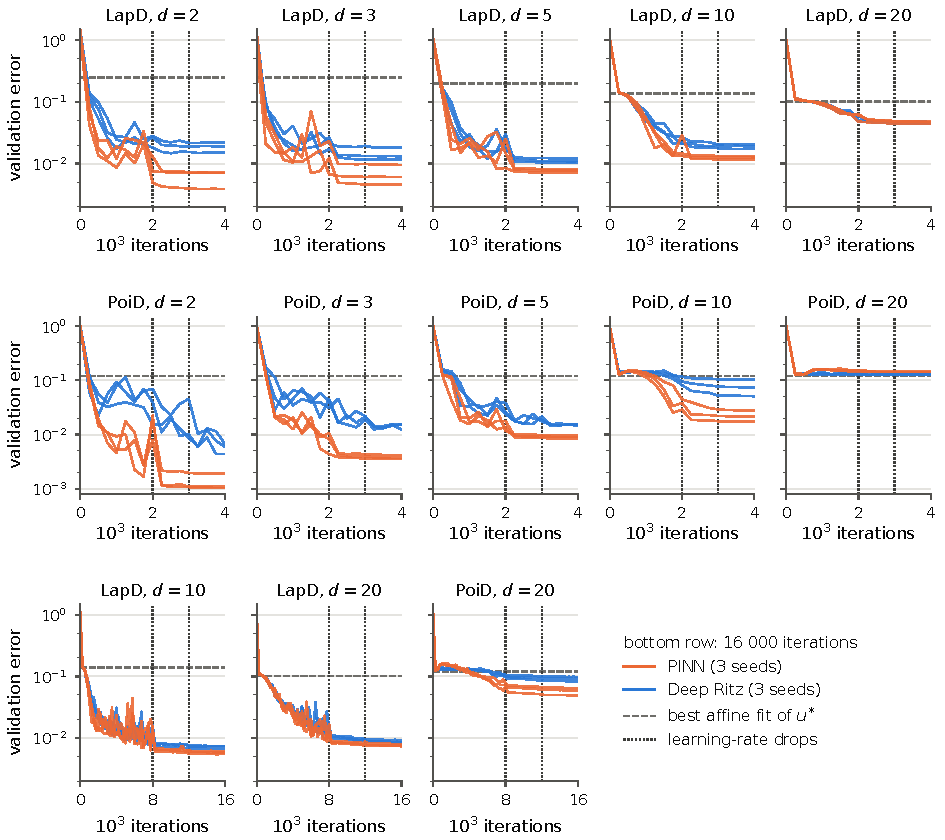
\includegraphics[width=\textwidth]{s6_highdim_curves.pdf}
\caption{Relative $L^2$ error on a validation set of 5000 points (distinct from the test
points), recorded every 250 iterations, for each of the three seeds; PINN in orange, Deep
Ritz in blue. Top two rows: the 4000-iteration runs of
Tables~\ref{s6_highdim:tab:p1} and~\ref{s6_highdim:tab:p2}. Bottom row: the
16\,000-iteration runs of Table~\ref{s6_highdim:tab:budget}. Dashed: error of the best
affine approximation of $\uex$. Dotted verticals: the learning-rate reductions at 50 and
75 per cent of the run.}
\label{s6_highdim:fig:curves}
% src: research_highdim/results/runs*.jsonl (curves); data/s6_highdim_long_d20.jsonl; data/closed_forms.json; script code/s6_highdim_figs.py
\end{figure}

\subsection{The networks at \texorpdfstring{$d=20$}{d = 20} and the effect of the budget}

% src: research_highdim/results/derived.txt (plateau block); data/s6_highdim_numbers.json (plateau_val_mean)
On \Ptwo\ at $d=10$ the mean validation error of Deep Ritz is $0.143$, $0.141$, $0.138$,
$0.137$ at iterations 250, 500, 1000, 1500 (Figure~\ref{s6_highdim:fig:curves}). On \Pone\ at
$d=20$ the descent has begun, but the learning-rate reduction at iteration 2000 arrests it
($0.111$ at iteration 250, $0.052$ to $0.057$ at 2000, $0.046$ to $0.047$ at 4000). The 1024
boundary points of an iteration are shared among 40 faces at $d=20$.
% src: research_highdim/results/extensions.json (d = 10); data/s6_highdim_long_d20.jsonl, data/s6_highdim_numbers.json (extensions, budget_ratios)
With 16\,000 iterations the errors at $d=10$ on \Pone\ are $\sci{5.88}{-3}$ (PINN) and
$\sci{7.28}{-3}$ (Deep Ritz), and at $d=20$ on \Pone\ $\sci{7.57}{-3}$ and $\sci{8.70}{-3}$
($\errC=\sci{2.8}{-2}$ and $\sci{3.2}{-2}$). On \Ptwo\ at $d=20$ the PINN seeds end at
$\sci{4.90}{-2}$, $\sci{6.58}{-2}$ and $\sci{6.02}{-2}$ and the Deep Ritz seeds at
$\sci{9.17}{-2}$, $\sci{9.87}{-2}$ and $\sci{8.26}{-2}$.
% src: data/s6_highdim_diag_d20.json (16 000-iteration networks)
The PINN's remainder after its affine fit now correlates 0.84 to 0.91 with that of $\uex$ and its
residual is 0.12 to 0.15; the Deep Ritz remainder has reached 0.63 to 0.76 of the right norm,
with residual 0.60 to 0.70. The lower residual of the PINN cannot by itself lower its error by
more than the bound of Remark~\ref{s6_highdim:rem:split}.

\subsection{Cost per iteration}\label{S5:sec:cost}

\begin{table}[tbp]
\centering
\caption{CPU time of one training iteration in milliseconds (one thread, network and
batch of Section~\ref{s6_highdim:sec}; median of 7 rounds of 10 iterations, the three variants
interleaved in every round) for Deep Ritz and for the PINN with the Laplacian computed by forward
propagation or by nested reverse-mode differentiation. ``Ratio'': time relative to Deep
Ritz, computed round by round; median, then [minimum, maximum]. Last column: nested divided
by forward (ratio of the medians). (a)~Timing of the primary study, load average about 90
to 110 on 12 cores. (b)~Second timing, made with separate code for the verification, load average
about 20; $d=3$ was not measured. Absolute times depend on the load.}
\label{s6_highdim:tab:cost}
\small
\setlength{\tabcolsep}{5pt}
% src (a): research_highdim/results/cost_vs_d.csv, cost_vs_d.json; load: data/checks/machine_load.json (highdim_cost_primary)
% src (b): verify_research_highdim/results/v_bench.txt, v_bench.json; load: data/checks/machine_load.json (highdim_cost_verification)
% generated by code/s6_highdim_tables.py -> data/s6_highdim_tables.tex
\begin{tabular}{@{}r r r r l r r l c@{}}
\toprule
 & Deep Ritz & \multicolumn{3}{c}{PINN, forward Laplacian} & \multicolumn{3}{c}{PINN, nested} & nested/\\
\cmidrule(lr){3-5}\cmidrule(lr){6-8}
$d$ & ms & ms & ratio & [min, max] & ms & ratio & [min, max] & forward\\
\midrule
\multicolumn{9}{@{}l}{\emph{(a) primary measurement}}\\
2 & 4.22 & 6.50 & 1.54 & [1.45, 1.64] & 7.48 & 1.72 & [1.56, 1.92] & 1.15 \\
3 & 4.33 & 7.06 & 1.62 & [1.50, 1.90] & 9.06 & 2.12 & [1.96, 2.26] & 1.28 \\
5 & 4.55 & 8.08 & 1.77 & [1.74, 1.90] & 12.47 & 2.70 & [2.56, 2.94] & 1.54 \\
10 & 4.68 & 10.66 & 2.23 & [2.10, 2.34] & 20.61 & 4.44 & [3.91, 4.53] & 1.93 \\
20 & 4.98 & 15.23 & 3.09 & [2.90, 3.16] & 37.80 & 7.72 & [7.11, 8.74] & 2.48 \\
50 & 8.02 & 48.82 & 6.11 & [5.66, 7.82] & 139.26 & 18.21 & [14.78, 19.94] & 2.85 \\
100 & 8.36 & 90.31 & 10.73 & [9.76, 15.19] & 243.45 & 29.46 & [23.55, 42.29] & 2.70 \\
\midrule
\multicolumn{9}{@{}l}{\emph{(b) second measurement (verification)}}\\
2 & 3.29 & 5.44 & 1.59 & [1.44, 1.82] & 6.09 & 1.81 & [1.67, 1.98] & 1.12 \\
5 & 3.69 & 6.47 & 1.87 & [1.65, 2.25] & 9.97 & 2.83 & [2.52, 3.17] & 1.54 \\
10 & 4.03 & 9.86 & 2.48 & [1.87, 2.99] & 17.93 & 4.39 & [3.55, 5.66] & 1.82 \\
20 & 4.47 & 14.26 & 3.15 & [2.54, 4.09] & 33.26 & 6.80 & [6.07, 9.09] & 2.33 \\
50 & 4.77 & 36.99 & 8.44 & [7.01, 8.70] & 76.74 & 16.71 & [14.00, 18.45] & 2.07 \\
100 & 5.12 & 69.03 & 13.34 & [12.00, 16.16] & 159.63 & 32.20 & [28.15, 35.47] & 2.31 \\
\bottomrule
\end{tabular}
\end{table}

\begin{figure}[tbp]
\centering
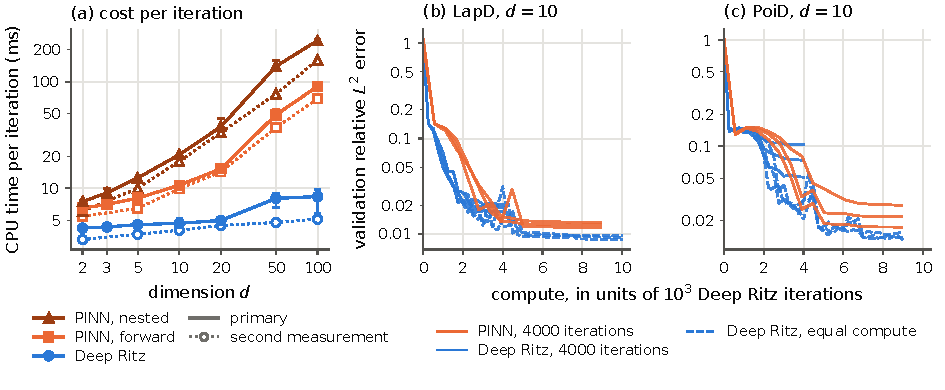
\includegraphics[width=\textwidth]{s6_highdim_cost.pdf}
\caption{(a)~CPU time per training iteration against $d$ (Table~\ref{s6_highdim:tab:cost}):
filled symbols and full lines are the primary measurement (median; bars from the fastest to
the slowest of 7 rounds), open symbols and dotted lines the second one.
(b,\,c)~Validation error (5000 points) against compute at $d=10$ for the three seeds of
each method. The abscissa counts compute in Deep Ritz iterations; one PINN iteration is
counted as 2.23 of them, the ratio of the primary measurement (with the ratio 2.48 of the
second measurement the PINN curves would end at 9.9 instead of 8.9). Dashed: Deep
Ritz with 10\,000 iterations (\Pone) and 9000 (\Ptwo).}
\label{s6_highdim:fig:cost}
% src: research_highdim/results/cost_vs_d.json; verify_research_highdim/results/v_bench.json; research_highdim/results/runs*.jsonl (phases main, equaltime); script code/s6_highdim_figs.py
\end{figure}

% src: data/s6_highdim_numbers.json (cost_growth_d2_to_d100, nested_over_fwd_d_ge_10, cost_primary, cost_verifier)
At $d=100$ the medians of the ratio of a PINN iteration to a Deep Ritz iteration are 10.7 and
13.3 with the forward Laplacian and 29.5 and 32.2 with the nested one; for $d\ge10$ the nested
Laplacian costs 1.9 to 2.9 and 1.8 to 2.3 times the forward one in the two measurements.
% src: verify_research_highdim/results/v_determinism.txt (seven reruns; CPU time 1.14 to 1.78 times the stored value); research_highdim/results/cost_vs_d.csv (Deep Ritz d = 100: rounds 5.79 to 9.75 ms)
Process CPU time on this machine depends on the load: seven training runs repeated bit for
bit took 1.1 to 1.8 times the CPU seconds stored for the originals. The Deep Ritz times of
the primary measurement at $d=50$ and $100$ (8.0 and 8.4\,ms, with rounds ranging from 5.8
to 9.7\,ms at $d=100$) appear inflated in this way; the quieter measurement gives 4.8 and
5.1\,ms.

\subsection{Equal compute}

% src: verify_research_highdim/results/v_summary.txt (rows 'equaltime', 'eq9k'); notes/VERIFICATION.md (sec. 3.1, V10; sec. 3.3, item 5)
With the smaller count of 9000 Deep Ritz iterations on \Pone\ at $d=10$, \textsf{V-dim} still
gives $\sci{9.24}{-3}$, $\sci{9.41}{-3}$, $\sci{9.65}{-3}$, below every PINN run
(Figure~\ref{s6_highdim:fig:cost}(b,\,c)). The equal-compute comparison was made in the study
only at $d=10$, with three seeds and three seeds of \textsf{V-dim}, and we do not extrapolate it:
the cost ratio grows with $d$ (Table~\ref{s6_highdim:tab:cost}), but so does the number of
iterations that either method needs (Table~\ref{s6_highdim:tab:budget}), and no equal-compute run
was made at the larger budget.

\subsection{Penalty weights and penalty bias}\label{S5:sec:weights}

% src: research_highdim/results/sweep.csv (val_rel_l2; d = 5, seed 100); rows generated by code/s6_highdim_tables.py
\begin{table}[tbp]
\centering
\caption{Choice of the weights at $d=5$: relative $L^2$ error on the validation set of
5000 points after 4000 iterations, in units of $10^{-2}$, for one run (seed 100) per
weight. The weight is $\lam$ for the PINN and $\bet$ for Deep Ritz; they are normalised
differently (Remark~\ref{s3_methods:rem:consistent}).}
\label{s6_highdim:tab:sweep}
\small
\setlength{\tabcolsep}{8pt}
\begin{tabular}{@{}lcccc@{}}
\toprule
 & \multicolumn{4}{c}{weight} \\
\cmidrule(l){2-5}
 & 1 & 10 & 100 & 1000 \\
\midrule
%% BEGIN GENERATED s6_highdim:tab:sweep
\Pone, PINN ($\lam$) & 1.03 & 0.917 & 0.792 & 0.716 \\
\Pone, Deep Ritz ($\bet$) & 16.0 & 2.33 & 1.03 & 1.10 \\
\Ptwo, PINN ($\lam$) & 4.08 & 1.31 & 1.12 & 0.976 \\
\Ptwo, Deep Ritz ($\bet$) & 1.60 & 1.61 & 1.68 & 1.68 \\
%% END GENERATED s6_highdim:tab:sweep
\bottomrule
\end{tabular}
\end{table}

The PINN on \Pone\ changes little with $\lam$ (Table~\ref{s6_highdim:tab:sweep}).
% src: verify_research_highdim/results/v_summary.txt (rows 'beta', 'lam1e4', 'main' at d = 10); notes/VERIFICATION.md (sec. 3.3, item 3: V11, V13)
At $d=10$ on \Ptwo\ (\textsf{V-dim}, seeds 7--9) Deep Ritz with $\bet=10$ or $100$ stays on the
affine plateau for the whole run ($\errL$ between $0.119$ and $0.126$, against $0.071$ to $0.096$
with $\bet=1$), and so does the PINN with $\lam=10^4$ ($0.111$ to $0.120$, against $0.021$ to
$0.026$ with $\lam=10^3$); on \Pone\ at $d=10$, $\lam=10^4$ is 14 per cent worse in the mean. A
large weight lengthens the plateau. Smaller values of $\lam$, and values of $\bet$ other than 100
on \Pone, were not tried at $d=10$.

\begin{table}[tbp]
\centering
\caption{Penalty bias of Deep Ritz on \Pone\ against the trained networks, $\bet=100$, in
units of $10^{-2}$. Bias: $\norm{\ubeta-\uex}/\norm{\uex}$
(Observation~\ref{sA_proofs:obs:biasd}). PINN, Deep Ritz: mean relative $L^2$ error of the
three seeds (Tables~\ref{s6_highdim:tab:p1} and~\ref{s6_highdim:tab:budget}); share: bias
over the Deep Ritz error, in per cent.}
\label{s6_highdim:tab:bias}
% src: data/s6_highdim_robin_bias.json (series: beta = 100; against_trained_networks); data/s6_highdim_robin_bias.txt; rows from data/s6_highdim_robin_bias_table.tex (code/s6_highdim_robin_bias.py)
\small
\setlength{\tabcolsep}{6pt}
\begin{tabular}{@{}rrrrrrrr@{}}
\toprule
 & & \multicolumn{3}{c}{4000 iterations} & \multicolumn{3}{c}{16\,000 iterations} \\
\cmidrule(lr){3-5}\cmidrule(l){6-8}
$d$ & bias & PINN & Deep Ritz & share & PINN & Deep Ritz & share \\
\midrule
2 & 0.548 & 0.608 & 1.882 & 29 & -- & -- & -- \\
3 & 0.470 & 0.672 & 1.421 & 33 & -- & -- & -- \\
5 & 0.299 & 0.760 & 1.113 & 27 & -- & -- & -- \\
10 & 0.146 & 1.260 & 1.896 & 8 & 0.588 & 0.728 & 20 \\
20 & 0.074 & 4.663 & 4.613 & 2 & 0.757 & 0.870 & 8 \\
\bottomrule
\end{tabular}
\end{table}

% src: verify_research_highdim/results/v_robin_fd.json (beta = 100: 5.48e-3; beta = 10: 5.002e-2); research_highdim/results/summary.csv (d = 2); verify_research_highdim/results/v_summary.txt (row 'robin', beta = 10: 4.775e-2); data/s6_highdim_robin_bias.json (against_trained_networks)
At $d=2$ on \Pone\ the minimiser of the penalised energy with $\bet=100$ is itself
$\sci{5.5}{-3}$ away from $\uex$ (Observation~\ref{s3_methods:obs:robin}). The bias is not a
lower bound for a run that has not converged, which can end on either side of it: the run with
$\bet=10$ of Observation~\ref{s3_methods:obs:robin} ends 4.5 per cent below the bias for that
$\bet$. After 16\,000 iterations the bias is 20 and 8 per cent of the Deep Ritz error at
$d=10$ and 20 (Table~\ref{s6_highdim:tab:bias}). By the triangle inequality the Deep Ritz
networks at $d=10$ are between $\sci{5.8}{-3}$ and $\sci{8.7}{-3}$ from their own target
$u_{\bet}$, against $\sci{5.9}{-3}$ for the distance of the PINN from $\uex$.

\subsection{The constant and the error bound: protocol, outcomes and re-checks}\label{S5:sec:bound}

\begin{table}[tbp]
\centering
\caption{The constant of Theorem~\ref{s6_highdim:thm:kappa}. $1/(2d)$ and $L_d$: proved lower
bounds of $\kappa_d^2$; ``comp.'': the largest Rayleigh quotient found on finite-dimensional
subspaces of sine modes, a lower bound of $\kappa_d^2$ up to rounding
(Observation~\ref{sA_proofs:obs:RR}); $U_d$: proved upper bound. $\sqrt{(1/2)/U_d}$: the factor by
which $\sqrt{U_d}$ improves Payne's constant $\sqrt{1/2}$. $\sqrt{2dU_d}$: factor of the
root-mean-square boundary misfit in Corollary~\ref{s6_highdim:cor:bound}(c). $2C_d$: the constant of
Proposition~\ref{s3_methods:prop:robin}(c) for the same map. $m_d$: the bound of $\kappa_d^2$ through
the torsion function of the cube (Remark~\ref{sA_proofs:rem:steklov}), computed by quadrature, and the
factor $\sqrt{m_d/U_d}$ by which $\sqrt{U_d}$ improves it.}
\label{s6_highdim:tab:kappa}
\footnotesize
\setlength{\tabcolsep}{3.8pt}
% src: research_highdim_bound/results/table_payne.tex (columns 1/(2d), L_d, U_d, sqrt((1/2)/U_d)); research_highdim_bound/results/table_theorem2.tex (computed, computed/U_d, sqrt(U_d), sqrt(2dU_d), 2C_d); research_highdim_bound/results/restricted_lanczos.txt; data/s6_highdim_torsion.json (m_d, sqrt(m_d/U_d); code/s6_highdim_torsion.py); rows written by code/s6_highdim_bound.py
\begin{tabular}{@{}rrrrrrrrrrrr@{}}
\toprule
$d$ & $1/(2d)$ & $L_d$ & comp. & $U_d$ & comp.$/U_d$ & $\sqrt{(1/2)/U_d}$ & $\sqrt{U_d}$ & $\sqrt{2dU_d}$ & $2C_d$ & $m_d$ & $\sqrt{m_d/U_d}$\\
\midrule
%% BEGIN GENERATED s6_highdim:tab:kappa
1 & 0.5000 & 0.5000 & 0.5000 & 0.5000 & 1.000 & 1.000 & 0.707 & 1.000 & 2.099 & 0.5000 & 1.000 \\
2 & 0.2500 & 0.1857 & 0.2875 & 0.2919 & 0.985 & 1.309 & 0.540 & 1.081 & 2.050 & 0.3377 & 1.075 \\
3 & 0.1667 & 0.1214 & 0.2120 & 0.2198 & 0.964 & 1.508 & 0.469 & 1.149 & 2.033 & 0.2819 & 1.132 \\
5 & 0.1000 & 0.0811 & 0.1477 & 0.1586 & 0.932 & 1.776 & 0.398 & 1.259 & 2.020 & 0.2350 & 1.217 \\
10 & 0.0500 & 0.0531 & 0.0927 & 0.1061 & 0.874 & 2.171 & 0.326 & 1.457 & 2.010 & 0.1953 & 1.357 \\
20 & 0.0250 & 0.0365 & 0.0581 & 0.0730 & 0.796 & 2.617 & 0.270 & 1.709 & 2.005 & 0.1703 & 1.527 \\
50 & 0.0100 & 0.0227 & 0.0314 & 0.0455 & 0.691 & 3.316 & 0.213 & 2.132 & 2.002 & 0.1485 & 1.807 \\
100 & 0.0050 & 0.0160 & 0.0204 & 0.0320 & 0.637 & 3.953 & 0.179 & 2.529 & 2.001 & 0.1366 & 2.066 \\
%% END GENERATED s6_highdim:tab:kappa
\bottomrule
\end{tabular}
\end{table}


% src: research_highdim_bound/PREREG_T2.md; notes/VERIFICATION.md (sec. 4.2: SHA-256 and date of the freeze); research_highdim_bound/results/inventory.json (88 checkpoints, 7 identical to pilot networks); research_highdim_bound/results/eval_pilot.jsonl; research_highdim_bound/results/eval_confirm.jsonl
\paragraph{Protocol.} The 88 saved networks are the main runs at $d=2,\dots,20$, the
16\,000-iteration and equal-compute runs at $d=10$ and the weight sweep at $d=5$. Besides H1 to
H3, two descriptive outputs were fixed before the confirmatory evaluation: $\eta$ and the share
against the penalty weight in the sweep at $d=5$ (H4), and a comparison with the bound from the
maximum principle. Thirteen networks of an earlier pilot had been evaluated before the freeze;
seven of the 88 saved networks are bit-identical to some of them and are treated as
non-confirmatory.

% src: research_highdim_bound/results/decisions.json (H1: violations [], min_z_D fresh 222.06, hd 75.49, min_eta 1.744; H2: n_tested 57, 21 failures, eta_range [1.744, 5.456]); research_highdim_bound/results/posthoc_analyses.json (eta_main_by_cell, d10 and d20: 1.927 to 2.760; poisson/ritz/d2 14.70-24.82); research_highdim_bound/results/table_budget.tex (16 000 iterations: 2.23 to 2.47)
\paragraph{Outcomes.} The margins of H1 are at least 222 standard errors on the new points and
75 on the test points. All failures of H2 are at $d=5$ except the three equal-compute Deep Ritz
networks of \Ptwo\ at $d=10$ ($\eta=3.36$ to $3.44$); at $d=2$ the efficiency of Deep Ritz on
\Ptwo\ is 14.7 to 24.8. For the 4000-iteration networks at $d=10$ and 20 and the
16\,000-iteration networks at $d=10$ the bound is within a factor 1.93 to 2.76 of the error
(Table~\ref{s6_highdim:tab:eta}).
% src: research_highdim_bound/results/posthoc_analyses.json (H2_share: failures 0.219-0.5741, passes 0.5726-0.986); notes/VERIFICATION.md (sec. 4.2)
No explanation of the failures was pre-registered or tested. The post-hoc conjecture that the
failures are exactly the networks with the smallest boundary shares does not hold: the share ranges
of failures and passes overlap.
% src: research_highdim_bound/results/decisions.json (H3); research_highdim_bound/results/share_by_d.csv; data/s6_highdim_bound_numbers.json (B_int_over_error_main_networks: d = 20 at most 0.355, d = 10 up to 0.805)
H3 holds also without the seven non-confirmatory networks. At $d=10$ the interior term
$B_{\mathrm{int}}$ is up to 0.81 of the error, so there Remark~\ref{s6_highdim:rem:split} does
not show the error to be dominated by the boundary misfit.
% src: research_highdim_bound/results/decisions.json (H4: rows by problem, method and weight; maxprinciple_over_L2bound: min 5.696, max 41.95)
In the weight sweep at $d=5$ (H4) a larger boundary weight lowers the boundary share and raises
$\eta$: for the PINN from 1.85 and 1.89 at weight 1 (share 0.97 and 0.99) to 4.15 and 3.02 at
weight 1000 (share 0.48 and 0.57) on \Ptwo\ and \Pone, and for Deep Ritz on \Pone\ from 1.74
(share 0.91) to 3.12 (share 0.41), while for Deep Ritz on \Ptwo\ $\eta$ stays between 4.99 and 5.46
(share 0.22 to 0.25). The sampled maximum-principle quantity
$\max_{\dOm}\abs{v-g}+\frac18\max_\Om\abs{\lap v+f}$, an upper bound of the error in the maximum
norm and hence in $L^2$ if the maxima were exact, was 5.7 to 42 times the bound of
Corollary~\ref{s6_highdim:cor:bound}(c) on these networks.
% src: research_highdim_bound/results/posthoc_analyses.json (d10_ordering: means_ordered_alike)
At $d=10$, descriptively, the seed-mean bound orders the two methods as the seed-mean error does,
on both problems, at equal iterations (PINN lower) and at equal compute (Deep Ritz lower).

% src: research_highdim_bound/check/out/c5_compare.json (eta_rel_diff_range [-0.0078, 0.0061]); research_highdim_bound/check/out/c4_fresh.jsonl (24 rows); research_highdim_bound/check/out_r2/r2_fresh.jsonl (21 rows); data/s6_highdim_bound_numbers.json (n_networks_bound_valid; recheck_r2: cells P1_ritz_eqcpu_d20, P1_pinn_d20, P1_ritz_d20)
\paragraph{Re-checks.} The re-check evaluated all 88 networks with its own network evaluator,
the Laplacian from the trace of the Hessian and new Monte-Carlo points. Its two rounds retrained
45 networks with separately written trainers and other seeds (24 and 21;
Section~\ref{sC_details:sec:verification}), on \Pone, \Ptwo\ and two problems outside the study,
for $d=2$ to 20 and including Deep Ritz at the CPU time of the PINN at $d=20$. At $d=20$ and equal
CPU time the second round gives Deep Ritz $\errL=0.0092$ to $0.0104$ after 12\,900 to 14\,600
iterations and the PINN $0.0459$ to $0.0484$ after 4000; at equal iterations Deep Ritz gives
$0.0456$ to $0.0514$.

\begin{table}[tbp]
\centering
\caption{Corollary~\ref{s6_highdim:cor:bound}(c) on the main networks (4000 iterations), new
Monte-Carlo set: mean over seeds 0--2 of the relative error, of the two absolute terms of the bound
and, with [minimum, maximum], of the efficiency $\eta$ and of the boundary share
$B_{\mathrm{bd}}/(B_{\mathrm{int}}+B_{\mathrm{bd}})$. The relative standard error of $\eta$ is at
most 0.33 per cent on this set.}
\label{s6_highdim:tab:eta}
\scriptsize
\setlength{\tabcolsep}{4pt}
% src: research_highdim_bound/results/table_eta_by_d.tex (generated by scripts/s8_tables.py from results/eval_confirm.jsonl); standard errors: research_highdim_bound/results/eval_summary.csv; rows written by code/s6_highdim_bound.py
\begin{tabular}{@{}llrrrrll@{}}
\toprule
problem & method & $d$ & $\errL$ & $B_{\mathrm{int}}$ & $B_{\mathrm{bd}}$ & $\eta$ [min, max] & share [min, max]\\
\midrule
%% BEGIN GENERATED s6_highdim:tab:eta
\Pone & PINN & 2 & $\sci{6.079}{-3}$ & $\sci{8.85}{-3}$ & $\sci{2.11}{-3}$ & 5.39 [5.24, 5.49] & 0.191 [0.186, 0.199] \\
\Pone & PINN & 3 & $\sci{6.704}{-3}$ & $\sci{5.42}{-3}$ & $\sci{3.37}{-3}$ & 3.97 [3.81, 4.07] & 0.391 [0.367, 0.437] \\
\Pone & PINN & 5 & $\sci{7.603}{-3}$ & $\sci{5.71}{-3}$ & $\sci{7.64}{-3}$ & 2.98 [2.89, 3.09] & 0.571 [0.546, 0.595] \\
\Pone & PINN & 10 & $\sci{1.254}{-2}$ & $\sci{6.00}{-3}$ & $\sci{3.10}{-2}$ & 2.20 [2.15, 2.23] & 0.838 [0.824, 0.857] \\
\Pone & PINN & 20 & $\sci{4.634}{-2}$ & $\sci{4.75}{-3}$ & $\sci{2.28}{-1}$ & 1.93 [1.93, 1.94] & 0.979 [0.977, 0.982] \\
\addlinespace
\Pone & Deep Ritz & 2 & $\sci{1.881}{-2}$ & $\sci{2.21}{-2}$ & $\sci{5.39}{-3}$ & 4.44 [3.86, 4.79] & 0.197 [0.189, 0.209] \\
\Pone & Deep Ritz & 3 & $\sci{1.421}{-2}$ & $\sci{1.42}{-2}$ & $\sci{5.58}{-3}$ & 4.27 [3.62, 4.63] & 0.282 [0.273, 0.288] \\
\Pone & Deep Ritz & 5 & $\sci{1.114}{-2}$ & $\sci{1.15}{-2}$ & $\sci{9.50}{-3}$ & 3.20 [3.14, 3.24] & 0.453 [0.435, 0.474] \\
\Pone & Deep Ritz & 10 & $\sci{1.888}{-2}$ & $\sci{1.58}{-2}$ & $\sci{3.83}{-2}$ & 2.13 [2.13, 2.13] & 0.708 [0.700, 0.721] \\
\Pone & Deep Ritz & 20 & $\sci{4.594}{-2}$ & $\sci{3.26}{-2}$ & $\sci{2.14}{-1}$ & 2.07 [2.06, 2.08] & 0.868 [0.859, 0.881] \\
\addlinespace
\Ptwo & PINN & 2 & $\sci{1.341}{-3}$ & $\sci{6.37}{-3}$ & $\sci{2.64}{-3}$ & 9.91 [8.02, 11.02] & 0.286 [0.250, 0.357] \\
\Ptwo & PINN & 3 & $\sci{3.753}{-3}$ & $\sci{7.95}{-3}$ & $\sci{6.47}{-3}$ & 5.43 [5.21, 5.86] & 0.449 [0.417, 0.466] \\
\Ptwo & PINN & 5 & $\sci{9.257}{-3}$ & $\sci{1.43}{-2}$ & $\sci{1.25}{-2}$ & 4.10 [4.03, 4.13] & 0.466 [0.449, 0.486] \\
\Ptwo & PINN & 10 & $\sci{2.181}{-2}$ & $\sci{1.06}{-2}$ & $\sci{2.99}{-2}$ & 2.65 [2.48, 2.76] & 0.736 [0.720, 0.762] \\
\Ptwo & PINN & 20 & $\sci{1.449}{-1}$ & $\sci{1.25}{-2}$ & $\sci{1.94}{-1}$ & 2.01 [2.01, 2.02] & 0.939 [0.939, 0.940] \\
\addlinespace
\Ptwo & Deep Ritz & 2 & $\sci{5.733}{-3}$ & $\sci{7.07}{-2}$ & $\sci{4.16}{-3}$ & 19.19 [14.70, 24.82] & 0.056 [0.050, 0.066] \\
\Ptwo & Deep Ritz & 3 & $\sci{1.424}{-2}$ & $\sci{6.52}{-2}$ & $\sci{1.10}{-2}$ & 7.60 [7.07, 8.31] & 0.144 [0.140, 0.149] \\
\Ptwo & Deep Ritz & 5 & $\sci{1.507}{-2}$ & $\sci{4.33}{-2}$ & $\sci{1.28}{-2}$ & 5.27 [5.11, 5.39] & 0.228 [0.219, 0.238] \\
\Ptwo & Deep Ritz & 10 & $\sci{7.509}{-2}$ & $\sci{3.80}{-2}$ & $\sci{8.08}{-2}$ & 2.25 [2.21, 2.27] & 0.674 [0.645, 0.701] \\
\Ptwo & Deep Ritz & 20 & $\sci{1.270}{-1}$ & $\sci{3.18}{-2}$ & $\sci{1.65}{-1}$ & 2.19 [2.18, 2.19] & 0.838 [0.838, 0.838] \\
%% END GENERATED s6_highdim:tab:eta
\bottomrule
\end{tabular}
\end{table}

\subsection{The unit square}\label{S5:sec:square}

% src: research_highdim_bound/results/posthoc_analyses.json (unit_square: lower_from_U2 3.42538, upper_from_lanczos 3.47876, lanczos_lam 0.287459, fgw2005_upper 3.47855)
For $d=2$ Theorem~\ref{s6_highdim:thm:kappa} gives $\delta_1\ge1/U_2>3.4253$. A Rayleigh
quotient bounds $\kappa_2^2$ from below, and hence $\delta_1$ from above, up to rounding and, where
quadrature is used, quadrature error. The largest one found on sine modes, 0.287459, gives
$\delta_1\le3.4788$, consistent with the published bound $\delta_1<1.96256$ for the square of area
$\pi$~\citep{ferrero2005fourth}, which is $\delta_1<3.4786$ after rescaling.
% src: research_highdim_bound/check/out_r2/r2_rr_quadrature.json (K20_nq200 0.28771205118818, nq400, nq800); research_highdim_bound/check/r2_rr_quadrature.py; data/s6_highdim_bound_numbers.json (unit_square: delta1_upper_from_it 3.47570, antunes_gazzola_rescaled 3.47718, antunes_gazzola_rel_above 4.27e-4); refs.bib (antunes2013convex, annote: 1.96179 for the square, n = 4, in the table of regular polygons)
A Rayleigh--Ritz computation on the harmonic side in the re-check (combinations of harmonic
extensions of sine modes on single sides, quadrature with 200, 400 and 800 nodes agreeing to
$10^{-13}$) gives the larger quotient 0.2877121, that is $\delta_1\le3.47570$. The value
$\delta_1\approx1.96179$ computed for the square of area $\pi$ by~\citet{antunes2013convex},
$\approx3.4772$ after rescaling by $\sqrt\pi$, lies $\sci{4.3}{-4}$ relative above this upper
bound, so it overestimates $\delta_1$ by at least $\sci{4.3}{-4}$ relative (up to the quadrature
error of the bound).

\subsection{The penalty bias, exactly}\label{S5:sec:bias}

% src: research_highdim_bound/results/exact_bias.jsonl; research_highdim_bound/results/bias_table.json
The exact representation of Proposition~\ref{sA_proofs:prop:exact} was evaluated on the grid
$d\in\{2,3,5,10,20,50,100\}$, $\bet\in\{1,3,10,100,10^3,10^4,10^5\}$
(Table~\ref{s6_highdim:tab:biasexact}).
For $\bet\le1000$ two truncations agree to $\sci{2.7}{-9}$ relative and a wider quadrature range
changes the entries by at most $\sci{1.0}{-8}$; at $\bet=10^4$ and $10^5$, computed with one
truncation, the wider range changes them by at most $\sci{4.5}{-5}$. The values agree with the
series values of Observation~\ref{sA_proofs:obs:biasd} to within $\sci{4.3}{-4}$ relative in all
20 shared cells, and with the finite-difference solution at $d=2$ (ratios 0.99998, 0.99992,
0.99989 for $\bet=10$, 100, 1000). The separately written implementation of the re-check
reproduces all 49 cells to within $\sci{3.9}{-5}$ relative.
% src: research_highdim_bound/results/exact_bias.jsonl (35 cells with beta <= 1000 at two truncations, nmax 5e4 and 2e5; 14 cells at beta = 1e4, 1e5 with one); research_highdim_bound/results/bias_table.json (max_trunc_diff 2.7e-9; exact_over_article_series 0.99957 to 1.00026; exact_over_fd); research_highdim_bound/results/exact_bias_wide_compare.json (max_rel_change_beta_le_1000 1.01e-8; max_rel_change_all 4.49e-5 at d = 100, beta = 1e5); research_highdim_bound/check/out/c2_bias.json; research_highdim_bound/check/out/c5_compare.json (bias_rel_diff_range up to 3.93e-5, bias_cells 49)
A first-order expansion $\ubeta-\uex=v_1/\bet+O(\bet^{-3/2})$ with an explicit remainder
(Theorem~\ref{sA_proofs:thm:first}) was checked through its consequence
$\abs{\norm{\ubeta-\uex}-\norm{v_1}/\bet}\le K_dN\bet^{-3/2}$, which holds in all 49 cells (the
norm of the remainder itself was not computed); its leading term overestimates the bias at
moderate $\bet$, the more so the larger $d$ (exact over leading term at $\bet=100$: 0.988 at $d=2$,
0.807 at $d=100$).
% src: research_highdim_bound/results/bias_table.tex (bound(b)/exact and article/exact at beta = 100); research_highdim_bound/results/bias_table.json (theorem1_all_ok: the difference of norms against K_d N beta^-1.5; ratio_exact_over_first); research_highdim_bound/scripts/s6_bias_table.py

\begin{table}[tbp]
\centering
\caption{Relative penalty bias $\norm{\ubeta-\uex}/\norm{\uex}$ of \Pone\ from
Proposition~\ref{sA_proofs:prop:exact}, and the ratio of two upper bounds to it at $\bet=1$ and
$\bet=100$: (b) the bound $\sqrt{U_d}\,\nbd{\dn\uex}/(2\bet)$ of
Corollary~\ref{s6_highdim:cor:bound}(b); (c) the bound $C_d\nbd{\dn\uex}/\bet$ of
Proposition~\ref{s3_methods:prop:robin}(c).}
\label{s6_highdim:tab:biasexact}
\small
\setlength{\tabcolsep}{4pt}
% src: research_highdim_bound/results/bias_table.tex (generated by scripts/s6_bias_table.py from results/exact_bias.jsonl); rows written by code/s6_highdim_bound.py
\begin{tabular}{@{}rrrrrrrrrr@{}}
\toprule
& \multicolumn{5}{c}{relative bias, $\bet=$} & \multicolumn{2}{c}{(b)/exact} & \multicolumn{2}{c}{(c)/exact}\\
\cmidrule(lr){2-6}\cmidrule(lr){7-8}\cmidrule(l){9-10}
$d$ & 1 & 3 & 10 & 100 & 1000 & $\bet=1$ & 100 & $\bet=1$ & 100\\
\midrule
%% BEGIN GENERATED s6_highdim:tab:biasexact
2 & $\sci{2.883}{-1}$ & $\sci{1.386}{-1}$ & $\sci{5.002}{-2}$ & $\sci{5.483}{-3}$ & $\sci{5.542}{-4}$ & 3.25 & 1.71 & 12.3 & 6.5 \\
3 & $\sci{2.534}{-1}$ & $\sci{1.181}{-1}$ & $\sci{4.244}{-2}$ & $\sci{4.698}{-3}$ & $\sci{4.760}{-4}$ & 3.21 & 1.73 & 13.9 & 7.5 \\
5 & $\sci{1.640}{-1}$ & $\sci{7.359}{-2}$ & $\sci{2.645}{-2}$ & $\sci{2.991}{-3}$ & $\sci{3.048}{-4}$ & 3.36 & 1.84 & 17.1 & 9.4 \\
10 & $\sci{7.837}{-2}$ & $\sci{3.383}{-2}$ & $\sci{1.232}{-2}$ & $\sci{1.463}{-3}$ & $\sci{1.513}{-4}$ & 3.99 & 2.14 & 24.6 & 13.2 \\
20 & $\sci{3.665}{-2}$ & $\sci{1.557}{-2}$ & $\sci{5.799}{-3}$ & $\sci{7.369}{-4}$ & $\sci{7.817}{-5}$ & 5.19 & 2.58 & 38.5 & 19.1 \\
50 & $\sci{1.233}{-2}$ & $\sci{5.240}{-3}$ & $\sci{2.007}{-3}$ & $\sci{2.812}{-4}$ & $\sci{3.155}{-5}$ & 7.87 & 3.45 & 73.9 & 32.4 \\
100 & $\sci{5.253}{-3}$ & $\sci{2.243}{-3}$ & $\sci{8.730}{-4}$ & $\sci{1.308}{-4}$ & $\sci{1.560}{-5}$ & 11.03 & 4.43 & 123.4 & 49.6 \\
%% END GENERATED s6_highdim:tab:biasexact
\bottomrule
\end{tabular}
\end{table}

\begin{conjecture}\label{s6_highdim:conj:dc}
For \Pone\ let $c(d)=\lim_{\bet\to\infty}\bet\norm{\ubeta-\uex}/\norm{\uex}$. Then
$d\,c(d)\to\sqrt{8/3}=1.632993\ldots$ as $d\to\infty$.
\end{conjecture}
\noindent Evidence (numerical, not a proof): from the exact representation at $\bet=10^9$,
extrapolated in the number of one-dimensional Robin roots ($2\times10^5$, $4\times10^5$,
$8\times10^5$), $d\,c(d)$ is 1.1098, 1.5276, 1.5200, 1.5773, 1.6112, 1.6222, 1.6294, 1.6319, 1.6326
and 1.6329 for $d=2$, 5, 10, 20, 50, 100, 300, $10^3$, $3\times10^3$ and $10^4$. The sequence is
not monotone ($d=5$ above $d=10$) and increases from $d=10$ on. The two extrapolations agree to
$\sci{2.5}{-5}$ relative, and without the extrapolation the values at large $d$ are too low.
% src: research_highdim_bound/results/dc_truncation.json; research_highdim_bound/results/dc_quadrature_check.json; notes/VERIFICATION.md (sec. 4.2)
A second computation, made in the re-check, expands $v_1=\lim_{\bet\to\infty}\bet(\ubeta-\uex)$ in
the Dirichlet sine basis, with the one-dimensional sums in closed form so that no modes are
truncated. It agrees with the values above to all printed digits and continues them: 1.632887 at
$d=10^4$, 1.632983 at $10^5$ and 1.632992 at $10^6$. A leading-order Laplace evaluation of the same
integral gives $\norm{v_1}^2\sim m/(12d)$ and $\norm{\uex}^2\sim m^2/16$ for the $m=\lfloor
d/2\rfloor$ products of \Pone, hence the limit $\sqrt{8/3}$; this asymptotic argument has not been
written out with error terms, so the statement remains a conjecture.
% src: research_highdim_bound/check/out_r2/r2_dc_theta.json (d_times_c: 1.63288654830 at d = 1e4, 1.63298250022 at 1e5, 1.63299209419 at 1e6; limit_sqrt_8_over_3 1.632993161855452); research_highdim_bound/check/r2_dc_theta.py (docstring: Laplace asymptotics)

\subsection{The two remedies: design and further results}\label{S5:sec:remedies}

\begin{table}[tbp]
\centering
\caption{The remedies at $d=20$, seeds 10--14: $\errL$ on the held-out test points in units of
$10^{-2}$, mean (sample standard deviation), and the seed-paired ratio
$\rho=\errL(\text{plain})/\errL(\text{arm})$: median [minimum, maximum] and the number of seeds with
$\rho>1$. ``eq.\ CPU'': the number of iterations (in brackets) that matches the CPU time of plain;
presolve on \Pridge\ with Deep Ritz was rerun with 3700 iterations because its 4000-iteration CPU
time exceeded plain by more than 5 per cent; elsewhere presolve's 4000-iteration runs are within 5
per cent of plain. f.-m.: feature-matched, excluded from the decision on the lift. The controls
lift3u and rep3 are in Table~\ref{sC_details:tab:controls}.}
\label{s6_highdim:tab:remedies}
\small
\setlength{\tabcolsep}{4pt}
% src: research_highdim_remedies/results/tables.tex (ratio columns, generated by scripts/analyze.py from results/summary.json); research_highdim_remedies/results/summary.json (error columns); rows written by code/s6_highdim_remedies.py
\begin{tabular}{@{}llllll@{}}
\toprule
problem & method & arm & iterations & $\errL$, mean (s.d.) & $\rho$: median [min, max], wins\\
\midrule
%% BEGIN GENERATED s6_highdim:tab:remedies
\Pone & Deep Ritz & plain & 4000 & 4.75 (0.37) & -- \\
\Pone & Deep Ritz & presolve & 4000 & 1.93 (0.55) & 2.67 [1.67, 3.40] 5/5 \\
\Pone & Deep Ritz & lift3c & 4000 & 2.04 (0.17) & 2.33 [2.08, 2.66] 5/5 \\
\Pone & Deep Ritz & lift3c & eq.\ CPU (3250) & 2.55 (0.22) & 1.85 [1.67, 2.13] 5/5 \\
\Pone & PINN & plain & 4000 & 4.80 (0.38) & -- \\
\Pone & PINN & presolve & 4000 & 1.82 (0.54) & 2.85 [1.72, 3.84] 5/5 \\
\Pone & PINN & lift3c & 4000 & 1.65 (0.10) & 2.86 [2.63, 3.36] 5/5 \\
\Pone & PINN & lift3c & eq.\ CPU (3650) & 1.87 (0.13) & 2.54 [2.34, 3.01] 5/5 \\
\midrule
\Ptwo\ (f.-m.) & Deep Ritz & plain & 4000 & 12.6 (0.037) & -- \\
\Ptwo\ (f.-m.) & Deep Ritz & presolve & 4000 & 12.7 (0.0079) & 1.00 [1.00, 1.00] 2/5 \\
\Ptwo\ (f.-m.) & Deep Ritz & lift3c & 4000 & 1.92 (0.025) & 6.59 [6.49, 6.69] 5/5 \\
\Ptwo\ (f.-m.) & Deep Ritz & lift3c & eq.\ CPU (3350) & 2.03 (0.016) & 6.22 [6.15, 6.28] 5/5 \\
\Ptwo\ (f.-m.) & PINN & plain & 4000 & 14.5 (0.28) & -- \\
\Ptwo\ (f.-m.) & PINN & presolve & 4000 & 15.4 (0.50) & 0.94 [0.91, 0.98] 0/5 \\
\Ptwo\ (f.-m.) & PINN & lift3c & 4000 & 1.07 (0.19) & 14.60 [10.35, 15.05] 5/5 \\
\Ptwo\ (f.-m.) & PINN & lift3c & eq.\ CPU (3550) & 1.18 (0.21) & 13.33 [9.53, 13.99] 5/5 \\
\midrule
\Pridge & Deep Ritz & plain & 4000 & 3.74 (0.33) & -- \\
\Pridge & Deep Ritz & presolve & 4000 & 10.2 (11) & 0.66 [0.14, 0.87] 0/5 \\
\Pridge & Deep Ritz & presolve & eq.\ CPU (3700) & 10.7 (11) & 0.59 [0.14, 0.80] 0/5 \\
\Pridge & Deep Ritz & lift3c & 4000 & 1.57 (0.082) & 2.27 [2.12, 2.75] 5/5 \\
\Pridge & Deep Ritz & lift3c & eq.\ CPU (3200) & 1.89 (0.096) & 1.91 [1.73, 2.26] 5/5 \\
\Pridge & PINN & plain & 4000 & 2.47 (0.16) & -- \\
\Pridge & PINN & presolve & 4000 & 3.18 (0.63) & 0.79 [0.63, 0.98] 0/5 \\
\Pridge & PINN & lift3c & 4000 & 1.47 (0.096) & 1.77 [1.45, 1.83] 5/5 \\
\Pridge & PINN & lift3c & eq.\ CPU (3750) & 1.54 (0.10) & 1.66 [1.39, 1.74] 5/5 \\
\midrule
\Pcospair & Deep Ritz & plain & 4000 & 20.6 (0.79) & -- \\
\Pcospair & Deep Ritz & presolve & 4000 & 20.6 (0.79) & 1.00 [1.00, 1.00] 0/5 \\
\Pcospair & Deep Ritz & lift3c & 4000 & 7.36 (0.30) & 2.83 [2.51, 2.94] 5/5 \\
\Pcospair & Deep Ritz & lift3c & eq.\ CPU (3350) & 8.13 (0.36) & 2.56 [2.25, 2.67] 5/5 \\
\Pcospair & PINN & plain & 4000 & 24.6 (0.78) & -- \\
\Pcospair & PINN & presolve & 4000 & 24.6 (0.78) & 1.00 [1.00, 1.00] 0/5 \\
\Pcospair & PINN & lift3c & 4000 & 6.11 (0.30) & 4.02 [3.83, 4.23] 5/5 \\
\Pcospair & PINN & lift3c & eq.\ CPU (3750) & 6.37 (0.31) & 3.85 [3.67, 4.06] 5/5 \\
%% END GENERATED s6_highdim:tab:remedies
\bottomrule
\end{tabular}
\end{table}


% src: research_highdim_remedies/PREREG_C1.md; research_highdim_remedies/PREREG_C1_P5.md; notes/VERIFICATION.md (sec. 4.3: hashes, freeze times and the later choices)
\paragraph{Design.} An exploratory lift1 arm on the first four problems was added after the
frozen analysis, and a fifth problem, with lift1 as a pre-registered arm, in a separately frozen
addendum; every later choice was recorded with its time. The network $\mathcal N$ of
Section~\ref{s6_highdim:sec} takes $\x\in[0,1]^d$ as it is; per-axis (separable)
networks~\citep{cho2023spinn} address the cost of high-dimensional collocation rather than the
plateau.
% src: research_highdim_remedies/results/repro_check.json (12 runs, test error and all weights identical)
The network, optimiser, schedule, point sampling and test sets are those of
Section~\ref{s3_methods:sec:highdim}, imported from the study's code, and the plain runs with
seeds 0 to 2 on \Pone\ and \Ptwo\ reproduce the runs of Tables~\ref{s6_highdim:tab:p1}
and~\ref{s6_highdim:tab:p2} at $d=20$ bit for bit.
% src: research_highdim_remedies/PREREG_C1.md (header; section 2.2); notes/VERIFICATION.md (sec. 4.3, pilots before the freeze); research_highdim_remedies/results/checks.json (C5_floors: laplace/d20, ridge/d20, cospair/d20, poisson/d20; exact_affine, exact_lift3)
Both remedies had been tried on \Pone\ and \Ptwo\ at $d=20$ in exploratory pilots with seeds 0 to
2 before the freeze, as had the centred input (on \Pone\ at $d=20$, on \Ptwo\ up to $d=16$) and,
for Deep Ritz on \Pone, rep3, so their direction on these two problems was known; only \Pridge\
and \Pcospair\ were held out. They have $f=16\uex$ (\Pridge) and $f=2\pi^2\uex$ (\Pcospair); a
related ridge had been used in an earlier pilot. On \Pone, \Pridge\ and \Pcospair\ an affine function of the
lift features approximates $\uex$ no better than an affine function of $\x$, or by about one per
cent: the relative floors at $d=20$ are $0.1015$ for both on \Pone, $0.7136$ and $0.7072$ on
\Pridge, and 1 and 1 on \Pcospair\ (Proposition~\ref{sA_proofs:prop:floorsC}). For the PINN the
affine part of presolve is the $L^2(\dOm)$ projection of $g$
(Proposition~\ref{sA_proofs:prop:presolve}).
% src: research_highdim_remedies/results/sweep_selection.json; research_highdim_remedies/PREREG_C1.md (section 2.3)
The Deep Ritz weight is that of the study on \Pone\ and \Ptwo\ ($\bet=100$ and $1$) and was chosen
by the same protocol on the held-out problems ($\bet=100$ on \Pridge, $1$ on \Pcospair); the PINN
uses $\lam=1000$ throughout.
% src: research_highdim_remedies/results/check_rep3_equivalence.json (8.9e-16 over 300 float64 steps)
Two controls were run for Deep Ritz only (Table~\ref{sC_details:tab:controls}): \emph{lift3u},
which spans the same functions as lift3c but uses the uncentred linear feature $x_i$ in place of
$P_1(t_i)$, and \emph{rep3}, the featureless input $(t,t,t)$. Under \Adam, rep3 is exactly the
centred-input network $\mathcal N(t)$ whose first-layer weight is trained with a three times
larger step and whose first bias starts with a third of the variance
(Proposition~\ref{sA_proofs:prop:rep3}); it is a reparametrisation control, not a pure control of
the number of inputs.
% src: research_highdim_remedies/results/eqcpu_plan.json; research_highdim_remedies/results/eqcpu_plan_p5.json; research_highdim_remedies/results/runs_d10.jsonl, runs_main20.jsonl (field cpu_shift_s: 0.000515 to 0.0358 s)
At equal CPU time lift3c runs fewer iterations (3200 to 3750 instead of 4000, schedule rescaled).
Presolve costs as much as plain per iteration, and its linear solve takes between 0.0005 and
0.036\,s of CPU time; its 4000-iteration runs count as equal-CPU runs where their CPU time is
within 5 per cent of plain, which held except for Deep Ritz on \Pridge, run again with 3700
iterations.

\begin{figure}[tbp]
\centering
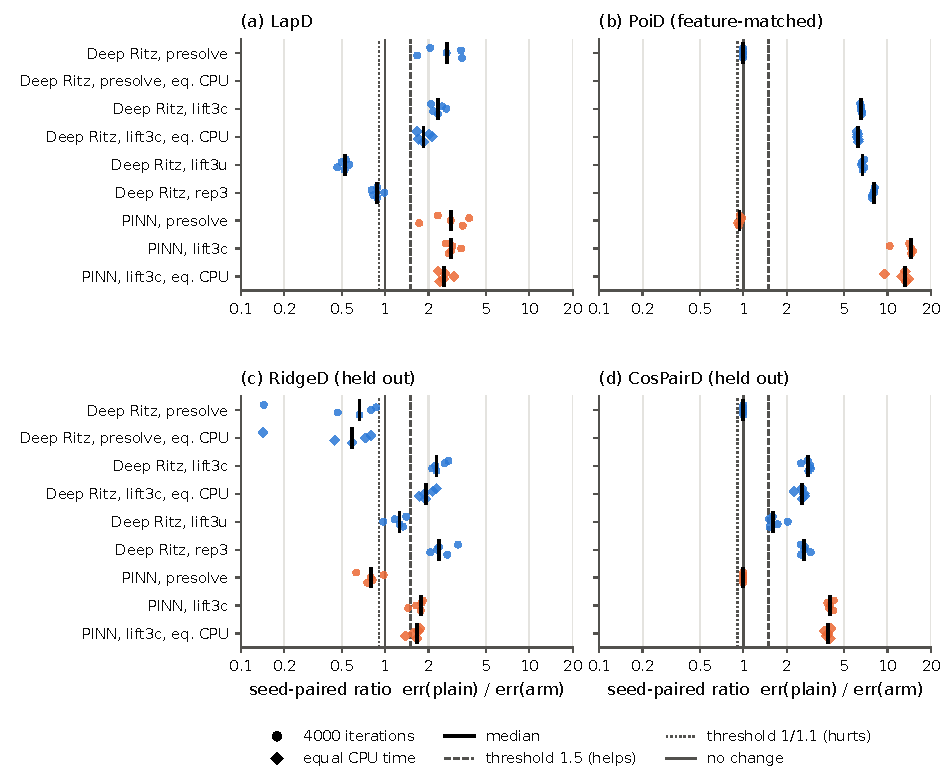
\includegraphics[width=\textwidth]{s6_remedies_ratios.pdf}
\caption{Seed-paired ratios $\rho=\errL(\text{plain})/\errL(\text{arm})$ at $d=20$ on the four
pre-registered problems, one row per method and arm, including the controls lift3u and rep3 (right
of 1: the arm is more accurate than plain). Circles: 4000 iterations; diamonds: equal CPU time;
bars: medians. Dashed: the threshold 1.5 of the decision rule; dotted: $1/1.1$.}
\label{s6_highdim:fig:remedies}
% src: research_highdim_remedies/results/summary.json; script code/s6_highdim_remedies.py (runs research_highdim_remedies/scripts/fig_ratios.py with the article's labels)
\end{figure}

% src: research_highdim_remedies/results/summary.json (P2, P3, P4 presolve); research_highdim_remedies/results/runs_main20.jsonl (ridge, ritz, seed 10); research_highdim_remedies/results/decision.json (stall: gamma_plain 0.902, 0.929, 0.841; gamma_presolve 0.054, 0.000, 0.000; rel_l2_plain, rel_l2_presolve)
\paragraph{Presolve.} On \Pridge\ one Deep Ritz run with presolve ends at an error of 0.295
against 0.042 without the shift (Figure~\ref{s6_highdim:fig:remedies}). In a secondary
pre-registered run with a constant learning rate and 12\,000 iterations presolve also suppressed
the late exit of Deep Ritz from the plateau on \Ptwo: the plain networks capture 84 to 93 per cent
of the non-affine part of $\uex$ (test errors 0.048 to 0.065), the shifted ones at most 5.4 per
cent (test errors 0.124 to 0.127; three seeds).

% src: research_highdim_remedies/results/decision.json (general_lift3c, per_problem; centring_clause: lift3c median 2.33, 5/5; lift3u median 0.52, 0/5; rep3_P1_descriptive); research_highdim_remedies/results/summary.json; research_highdim_remedies/results/summary_exploratory.json (lift1); research_highdim_remedies/results/attribution.json
\paragraph{Lift.} The median ratios of lift3c over plain are 2.33 and 2.86 on \Pone, 2.27 and
1.77 on \Pridge, 2.83 and 4.02 on \Pcospair\ (Deep Ritz and the PINN) at 4000 iterations, 1.85
and 2.54, 1.91 and 1.66, 2.56 and 3.85 at equal CPU time, and 6.59 and 14.60 on the
feature-matched \Ptwo. On \Pone\ the uncentred variant lift3u is less accurate than plain in 5 of
5 seeds (median 0.52), so the pre-registered centring clause was triggered and no statement about
the Legendre features is made from it. Centring alone does not give the gain on \Pone\ either:
lift1 gives 0.92 (2 of 5 seeds better) for Deep Ritz and rep3 0.88 (0 of 5), whereas lift1 gives
1.78 (5 of 5) for the PINN.
% src: research_highdim_remedies/results/attribution.json; research_highdim_remedies/results/summary_exploratory.json; research_highdim_remedies/results/summary.json (rep3, lift3c); notes/VERIFICATION.md (sec. 4.3, later choice 2)
Against the exploratory lift1 arm (Table~\ref{s6_highdim:tab:remedies5}(b)), lift3c is more
accurate on \Pone\ (median ratio 2.43 for Deep Ritz, 1.61 for the PINN) and on \Pcospair\ (2.23
and 2.39), 5 of 5 seeds each, but not on \Pridge\ (0.98 with 1 of 5 seeds better, and 0.77 with 0
of 5): there the whole gain of lift3c over plain is matched by centring the input (lift1 against
plain: 2.38 and 2.22, 5 of 5). On \Ptwo, \Pridge\ and \Pcospair\ rep3 gains about as much as
lift3c for Deep Ritz (medians 8.10, 2.37, 2.65 against 6.59, 2.27, 2.83).

% src: research_highdim_remedies/results/check_p5_formulas.json; research_highdim_remedies/results/checks_p5.json (C5); research_highdim_remedies/check/reimpl_summary.txt; research_highdim_remedies/PREREG_C1_P5.md; notes/VERIFICATION.md (sec. 4.3); research_highdim_remedies/results/sweep_selection_p5.json
\paragraph{A fifth problem.} \Paltridge\ is $\uex=\cos(\pi s'+1)$ with
$s'=d^{-1/2}\sum_ie_i(2x_i-1)$, $e_i=+1$ for odd and $-1$ for even $i$, and $f=4\pi^2\uex$; its
affine floor at $d=20$ is $0.8965$ and the floor of the lift features $0.8951$
(Proposition~\ref{sA_proofs:prop:floorsC}(e)). It was run with seeds 10 to 14, both remedies and
the arms lift3u, rep3 and lift1, with $\bet=1000$ chosen by the same protocol.
% src: research_highdim_remedies/results/decision_p5.json; research_highdim_remedies/results/summary_p5.json; research_highdim_remedies/results/eqcpu_plan_p5.json; research_highdim_remedies/results/attribution.json (P5)
For the PINN at equal CPU time lift3c runs 3700 iterations (median ratio 0.72, 0 of 5 seeds
better; 0.88 with 1 of 5 at 4000 iterations); for Deep Ritz 3200 (0.32). For Deep Ritz with three
seeds the sign is the same at $d=10$ (0.65) and $d=5$ (0.39), 0 of 3 seeds better in both.
Presolve gives 0.73 for Deep Ritz and 0.83 for the PINN, 1 of 5 each (CPU time 1.042 and 1.012
times plain, so its 4000-iteration runs count as equal-CPU runs). Against lift1, lift3c is less
accurate on \Paltridge\ for both methods (0.69 with 1 of 5 seeds, 0.68 with 0 of 5)
(Table~\ref{s6_highdim:tab:remedies5}, Figure~\ref{s6_highdim:fig:altridge}).
% src: research_highdim_remedies/results/decision_p5.json (extended_verdict_P1_P5); research_highdim_remedies/results/check_harness_after_p5.json; research_highdim_remedies/results/checks_p5.json (C6)
The frozen verdict that lift3c is a general remedy holds on \Pone, \Pridge\ and \Pcospair\ only.
The code paths of the first four problems were unchanged by the addition of the fifth: one stored
plain run and one stored lift1 run were reproduced bit for bit afterwards.

\begin{table}[tbp]
\centering
\caption{(a) \Paltridge\ at $d=20$, seeds 10--14, quantities and units as in
Table~\ref{s6_highdim:tab:remedies}; pre-registered in the addendum, not blind. (b) The lift
against the centred-input network lift1 $=\mathcal N(2\x-1)$ at $d=20$: median [minimum, maximum]
of the seed-paired ratio and the number of seeds with ratio above 1. The lift1 arm is exploratory
on \Pone\ to \Pcospair\ and pre-registered on \Paltridge.}
\label{s6_highdim:tab:remedies5}
\small
\setlength{\tabcolsep}{4pt}
% src: research_highdim_remedies/results/tables_p5.tex (generated by scripts/analyze_p5.py from results/summary_p5.json and results/attribution.json); research_highdim_remedies/results/summary_p5.json (error column of (a)); rows written by code/s6_highdim_remedies.py
\begin{tabular}{@{}lllll@{}}
\multicolumn{5}{@{}l}{\emph{(a) \Paltridge, $d=20$}}\\
\toprule
method & arm & iterations & $\errL$, mean (s.d.) & $\rho$: median [min, max], wins\\
\midrule
%% BEGIN GENERATED s6_highdim:tab:altridge
Deep Ritz & plain & 4000 & 2.27 (0.11) & -- \\
Deep Ritz & presolve & 4000 & 4.84 (3.2) & 0.73 [0.22, 1.10] 1/5 \\
Deep Ritz & lift3c & 4000 & 3.81 (0.36) & 0.59 [0.57, 0.64] 0/5 \\
Deep Ritz & lift3c & eq.\ CPU (3200) & 7.11 (0.57) & 0.32 [0.30, 0.35] 0/5 \\
Deep Ritz & lift3u & 4000 & 2.77 (0.36) & 0.82 [0.66, 1.01] 1/5 \\
Deep Ritz & rep3 & 4000 & 2.59 (0.55) & 0.93 [0.62, 1.19] 1/5 \\
Deep Ritz & lift1 & 4000 & 2.86 (0.64) & 0.84 [0.57, 1.01] 1/5 \\
PINN & plain & 4000 & 1.30 (0.067) & -- \\
PINN & presolve & 4000 & 1.61 (0.32) & 0.83 [0.69, 1.01] 1/5 \\
PINN & lift3c & 4000 & 1.45 (0.083) & 0.88 [0.80, 1.01] 1/5 \\
PINN & lift3c & eq.\ CPU (3700) & 1.76 (0.16) & 0.72 [0.68, 0.87] 0/5 \\
PINN & lift1 & 4000 & 1.01 (0.048) & 1.29 [1.21, 1.36] 5/5 \\
%% END GENERATED s6_highdim:tab:altridge
\bottomrule
\end{tabular}

\medskip
\begin{tabular}{@{}llll@{}}
\multicolumn{4}{@{}l}{\emph{(b) lift3c against lift1, $d=20$, 4000 iterations}}\\
\toprule
problem & method & $\errL(\text{lift1})/\errL(\text{lift3c})$ & $\errL(\text{plain})/\errL(\text{lift1})$\\
\midrule
%% BEGIN GENERATED s6_highdim:tab:lift1
\Pone & Deep Ritz & 2.43 [1.92, 2.99] 5/5 & 0.92 [0.83, 1.17] 2/5 \\
\Pone & PINN & 1.61 [1.24, 2.01] 5/5 & 1.78 [1.46, 2.27] 5/5 \\
\Ptwo & Deep Ritz & 4.22 [3.62, 4.79] 5/5 & 1.57 [1.39, 1.80] 5/5 \\
\Ptwo & PINN & 7.51 [4.74, 8.15] 5/5 & 1.95 [1.85, 2.19] 5/5 \\
\Pridge & Deep Ritz & 0.98 [0.88, 1.09] 1/5 & 2.38 [2.15, 3.12] 5/5 \\
\Pridge & PINN & 0.77 [0.74, 0.90] 0/5 & 2.22 [1.89, 2.39] 5/5 \\
\Pcospair & Deep Ritz & 2.23 [1.72, 2.36] 5/5 & 1.30 [1.25, 1.46] 5/5 \\
\Pcospair & PINN & 2.39 [1.99, 2.52] 5/5 & 1.70 [1.63, 1.92] 5/5 \\
\Paltridge & Deep Ritz & 0.69 [0.56, 1.09] 1/5 & 0.84 [0.57, 1.01] 1/5 \\
\Paltridge & PINN & 0.68 [0.65, 0.74] 0/5 & 1.29 [1.21, 1.36] 5/5 \\
%% END GENERATED s6_highdim:tab:lift1
\bottomrule
\end{tabular}
\end{table}

\begin{figure}[tbp]
\centering
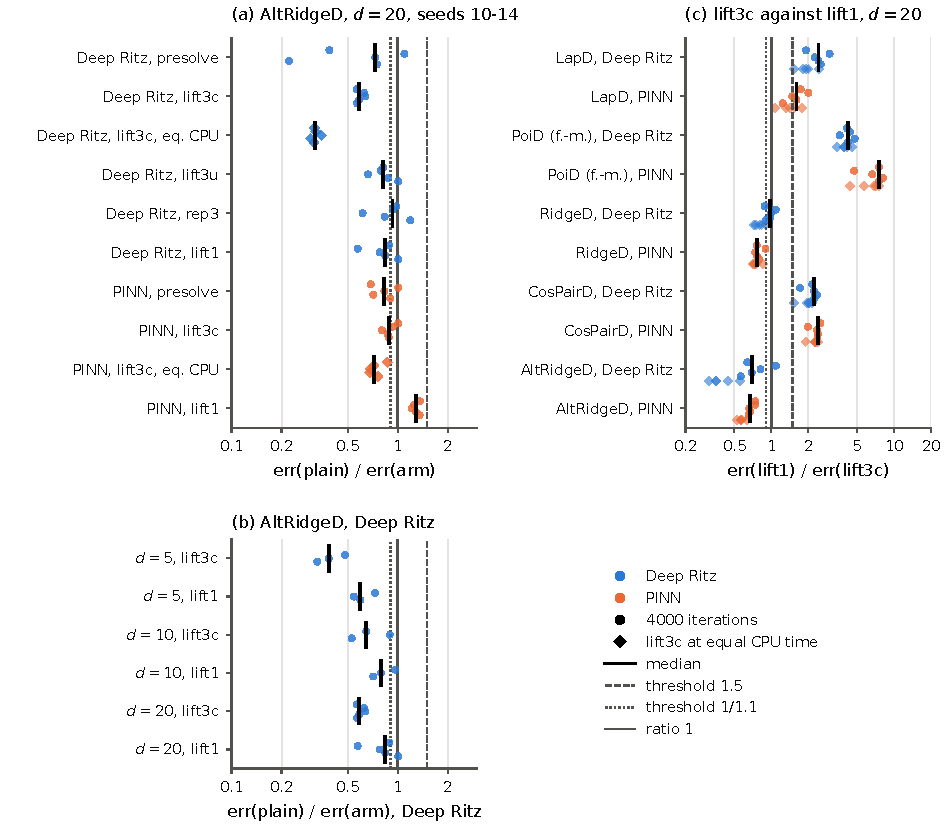
\includegraphics[width=\textwidth]{s6_remedies_altridge.pdf}
\caption{(a) Seed-paired ratios on \Paltridge\ at $d=20$; (b) \Paltridge, Deep Ritz, lift3c and lift1
against plain at $d=5$, 10 and 20 (three seeds at $d=5$ and 10); (c) the lift against the
centred-input network, $\errL(\text{lift1})/\errL(\text{lift3c})$, on the five problems at $d=20$
(diamonds: lift3c at equal CPU time). Lines as in Figure~\ref{s6_highdim:fig:remedies}.}
\label{s6_highdim:fig:altridge}
% src: research_highdim_remedies/results/summary_p5.json; research_highdim_remedies/results/attribution.json; script code/s6_highdim_remedies.py (runs research_highdim_remedies/scripts/fig_p5_baseline.py with the article's labels)
\end{figure}

\paragraph{Two further problems.} The second round of the re-check, under a plan frozen before its
runs, used fresh seeds 40 to 42 and two problems on which neither remedy had been tried before:
\Psinlin, $\uex=\sum_{k\le d/2}\sin(\pi x_{2k-1})\,x_{2k}$ with $f=\pi^2\uex$, and
\Pexpcos, $\uex=\sum_{k\le d/2}\ee^{x_{2k-1}}\cos(x_{2k})$ with $f=0$. Their relative affine
floors are 0.172 and 0.022 and the floors of the lift features 0.086 and 0.015 (Monte Carlo), so
on \Psinlin\ the best affine function of the lift features has half the error of the best affine
function of $\x$. The Deep Ritz weight was chosen by the study's protocol on that code's own
validation set ($\bet=100$ and 1000).
% src: notes/VERIFICATION.md (sec. 4.3: plan of the second round, its hash and time); research_highdim_remedies/check/selftest2.json (P6_floor_affine 0.1716, P6_floor_lift3 0.0861, P7_floor_affine 0.0224, P7_floor_lift3 0.0149); research_highdim_remedies/check/reimpl2.py; data/s6_highdim_remedies_recheck.json (beta_selected: P6 100, P7 1000, from the sweep runs in research_highdim_remedies/check/runs_reimpl2.jsonl)
For Deep Ritz at $d=20$ (three seeds each, seed-paired ratios against plain): on \Psinlin\ lift3c
gives 2.94 (3 of 3 seeds better), 2.53 at equal CPU time (3350 iterations) and 2.14 at $d=10$, but
the centred-input network lift1 alone gives 3.02, and lift3c against lift1 gives 1.01, so the whole
gain is matched by centring; presolve gives 1.16 (3 of 3, below the threshold 1.5 of the plan). On
\Pexpcos, which is on the plateau ($\errL=0.025$ for plain, affine floor 0.022), presolve gives
4.51 ($\errL=0.0053$ to $0.0063$), lift3c 1.85 and lift1 1.33 (3 of 3 each), and lift3c against
lift1 1.34. For the PINN on \Pone\ at $d=20$, that code gives ratios of the same size as the study's
(presolve 2.81 and 3.96, lift3c 2.86 and 2.68 for seeds 40 and 41; study medians 2.85 and 2.86). Not all runs of the plan were made: the third
seed of this PINN cell, its equal-CPU runs and the PINN on \Psinlin\ are missing. These results are
descriptive, from a different implementation, and are not part of the pre-registered study.
% src: research_highdim_remedies/check/runs_reimpl2.jsonl; research_highdim_remedies/check/reimpl2_summary.json; research_highdim_remedies/results/tables.tex (study medians, P1 PINN: presolve 2.85, lift3c 2.86); data/s6_highdim_remedies_recheck.json (recomputed by code/s6_highdim_remedies.py: P6 lift3c 2.937, eq. CPU 2.533, d10 2.140, lift1 3.018, lift1/lift3c 1.011, presolve 1.163; P7 presolve 4.507, lift3c 1.852, lift1 1.333, lift1/lift3c 1.336, plain err 0.02504-0.02532; P1 PINN presolve 2.814, 3.961, lift3c 2.858, 2.677; missing runs)

% src: research_highdim_remedies/results/decision.json; research_highdim_remedies/results/decision_p5.json; research_highdim_remedies/results/attribution.json; data/s6_highdim_remedies_recheck.json
\paragraph{Counts over seven problems.} Counting the two problems of the second round of the
re-check (Deep Ritz only, three seeds), presolve is clearly more accurate than plain on two of
seven problems (\Pone, \Pexpcos), close to plain on three (\Ptwo, \Pcospair, \Psinlin) and less
accurate on two (\Pridge, \Paltridge); lift3c is more accurate than plain on six and less accurate
on one (\Paltridge), but on two of the six (\Pridge\ and \Psinlin) centring the input alone gives
as much or more.
% src: research_highdim_remedies/results/summary.json (plain, d20); research_highdim_remedies/results/summary_p5.json (plain, d20); research_highdim_remedies/results/checks.json (C5_floors: test_affine); research_highdim_remedies/results/checks_p5.json (C5)
On \Pone, \Pridge, \Pcospair\ and \Paltridge\ plain ends below the affine floor (Deep Ritz 0.048,
0.037, 0.206, 0.023; PINN 0.048, 0.025, 0.246, 0.013; floors on the test set 0.102, 0.715, 1.000,
0.900).
% src: data/s6_highdim_remedies_recheck.json (P7/ritz/d20: plain_err 0.02504-0.02532, presolve/4000 median 4.507; P6/ritz/d20: plain_err 0.0997-0.1155); research_highdim_remedies/check/selftest2.json (P7_floor_affine 0.0224, P6_floor_affine 0.1716); research_highdim_remedies/results/summary_p5.json (plain, d20); research_highdim_remedies/results/checks_p5.json (C5)
Of the problems added after the pre-registered test, only \Pexpcos\ (Deep Ritz, three seeds, a
different implementation, descriptive) is on the plateau ($\errL=0.025$ for plain, affine floor
0.022), and presolve is 4.51 times more accurate there.
% src: research_highdim_remedies/results/summary.json (P1/d10 ... P4/d10, paired medians)
A descriptive check at $d=10$ with Deep Ritz and three seeds shows the same signs on \Pone\ to
\Pcospair\ (presolve: 1.62 on \Pone, 0.87 on \Ptwo, 0.74 on \Pridge, 1.00 on \Pcospair; lift3c:
1.38, 4.87, 2.01, 4.68).
% src: data/s6_highdim_remedies_recheck.json (load1_range over the field load1 of research_highdim_remedies/results/runs_*.jsonl: 6.8 to 166.3)
Every run was made serially on a shared 12-core laptop whose one-minute load average ranged from
about 7 to 166 during the runs, which affects the CPU-time measurements, and the cells at $d=5$ and
$10$ have three seeds and are descriptive.

% =====================================================================================
% sections/S6_pitfalls.tex -- Supplementary Section S6: details of the two demonstrations of
% Section 7.  Script: code/s7_pitfalls.py (-> data/s7_pitfalls_autograd.json, figures/s7_pitfalls.pdf);
% research_benchmark/scripts/run_oneface.py (-> research_benchmark/results/oneface_laplace3d.json).
% All "% src:" paths are relative to the root of the repository.
% =====================================================================================
\section{Implementation pitfalls: details of the demonstrations}\label{S6:sec}

\subsection{Differentiating with respect to a slice of the input}

\begin{lstlisting}[float=tp,captionpos=b,label={s7_pitfalls:lst:autograd},caption={The second time derivative computed with respect to a slice of the input (faulty) and with respect to the whole input (correct). The comments at the right give what the faulty lines return. Both patterns are executed by \texttt{code/s7\_pitfalls.py}.}]
# faulty: txy[:, 0] is a new tensor on which u_t does not depend
h = torch.autograd.grad(u_t, txy[:, 0], grad_outputs=torch.ones_like(u_t),
                        create_graph=True, allow_unused=True)[0]  # None
u_tt = torch.zeros_like(u_t) if h is None else h[:, 0]            # zeros
# correct: differentiate w.r.t. the whole input, then index
h = torch.autograd.grad(u_t.sum(), txy, create_graph=True)[0]     # (N, 3)
assert h is not None
u_tt = h[:, 0]
\end{lstlisting}

% src: code/s7_pitfalls.py; data/s7_pitfalls_autograd.json (protocol; autograd_demo: slice_grad_is_None true, none_returns_per_call 3, without_allow_unused_raises, max_abs_residual_faulty 0.0, residual_faulty_requires_grad false)
Listing~\ref{s7_pitfalls:lst:autograd} shows the two patterns for $u_{tt}$; the spatial second
derivatives are treated alike. On the untrained network and 64 points, the faulty operator returns
\code{None} in all three second-derivative calls and a residual that is exactly zero and does not
even require a gradient, and the call without \code{allow_unused} raises the error that the
differentiated tensor does not appear in the graph.

\paragraph{The training run.} The network is $3$--$50$--$50$--$1$ with tanh activations; the
10\,000 training points are independent and uniform in $[0,1]\times[-1,1]^2$; the loss is the sum
of the mean squared faulty residual, the mean squared difference from $\ee^{-t}S$ at the points of
the batch, with $S=\sin(\pi x)\sin(\pi y)$, and the mean squared value at 400 points on the spatial
boundary at $t=0$. Batches of 64 are drawn by a permutation per pass; \Adam\ with learning rate
$10^{-3}$, seed 0, 150 passes, that is 23\,550 iterations, on one CPU thread.
% src: data/s7_pitfalls_autograd.json (slices at t = 0, 1, 2, 3: amplitude 0.98110, 0.36431, 0.10037, 0.04399; no sign change on [0,3]; rel_L2_vs_exact 1.998 at t = 0.5, 2.369 at t = 1)
% src: data/closed_forms.json (wave2d: exp_minus_t_at_t_1_2_3, exact_factor_at_t_1_2_3)
The least-squares amplitude of the mode, $a(t)=\ip{\unet(t,\cdot)}{S}/\ip{S}{S}$, is 0.981, 0.364,
0.100 and 0.044 at $t=0,1,2,3$, against $\ee^{-t}=1$, 0.368, 0.135, 0.050 and against the factor
$\cos(\sqrt2\,\pi t)=1$, $-0.266$, $-0.858$, $+0.723$ of the solution of \PWtwo\
(Figure~\ref{s7_pitfalls:fig:demo}(a); the times 2 and 3 lie outside the sampled window). It never
changes sign. The relative $L^2$ distance from the solution of \PWtwo\ is 2.0 on the slice $t=0.5$
and 2.4 on the slice $t=1$.
% src: data/s7_pitfalls_autograd_1500passes.json (slices at t = 0, 1, 2, 3: amplitude 0.99734, 0.36831, 0.14998, 0.07667; heldout_21x81x81: 0.0059 vs target)
With 1500 passes the amplitudes are 0.997 and 0.368 at $t=0$ and $1$ (0.150 and 0.077 at $t=2$
and $3$), and the distance from $\ee^{-t}S$ on the held-out grid is 0.006. The PDE term is zero
whatever the number of passes, because the missing derivative does not depend on the weights.

\begin{figure}[tbp]
\centering
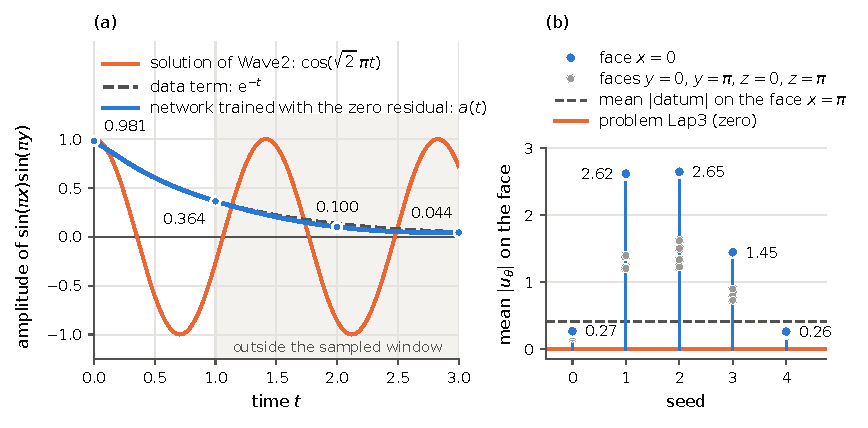
\includegraphics[width=\textwidth]{s7_pitfalls.pdf}
\caption{The two demonstrations of Section~\ref{s7_pitfalls:sec}.
(a)~Residual made identically zero by differentiation with respect to a slice of the input:
least-squares amplitude $a(t)=\ip{\unet(t,\cdot)}{S}/\ip{S}{S}$ of the mode
$S=\sin(\pi x)\sin(\pi y)$, on a $101\times101$ grid per time, for the network trained with the
zero residual and the data term $\ee^{-t}S$ (seed 0, 150 passes, that is 23\,550 \Adam\
iterations), with the factor $\cos(\sqrt2\,\pi t)$ of the solution of \PWtwo; dots mark
$t=0,1,2,3$. Training samples $t\in[0,1]$; the shaded region lies outside that window.
(b)~Laplace problem with data on one face only: mean of $\abs{\unet}$ over $20\times20$ points of
the face $x=0$ (blue, value printed) and of each of the four other faces without a condition
(grey), for five seeds. The solution of \PLthree, which has zero data on these faces, vanishes on
all five; the dashed line is the mean of the datum $\abs{\sin y\cos z}$ over the constrained face,
$4/\pi^2\approx0.41$, for scale.}
% src: data/s7_pitfalls_autograd.json (panel a); research_benchmark/results/oneface_laplace3d.json (oneface_laplace3d.rows, panel b); script code/s7_pitfalls.py
\label{s7_pitfalls:fig:demo}
\end{figure}

\subsection{The problem with data on one face}

% src: research_benchmark/results/oneface_laplace3d.json (device mps; interior_seed_std_over_rms_exact 4.49); research_benchmark/scripts/run_oneface.py
The five networks of Section~\ref{s7_pitfalls:sec:oneface} were trained as one stack on the GPU
backend, with the loss $\operatorname{mean}(\lap\unet)^2+\operatorname{mean}(\unet-\text{datum})^2$
over the 9261 grid points and the 441 points of the face $x=\pi$, AdamW~\citep{loshchilov2019} with its default weight
decay 0.01, single precision; their predictions are compared with the solution of \PLthree\ on its
$40^3$ cell-centred evaluation grid. The pointwise standard deviation of the five predictions over
the seeds, averaged over that grid, is 4.49 times the root-mean-square value of the solution of
\PLthree.

% =====================================================================================
% sections/S7_proofs.tex -- Supplementary Section S7: proofs of the propositions fixed in
% statements.tex.  The propositions are referred to by their fixed labels and are not
% restated.  All `% src:` paths are relative to the root of the repository.
% Every computational step of Sections S7.1-S7.4 and S7.7 is cross-checked by code/sA_proofs_checks.py
% (output: data/sA_proofs_checks.json and data/sA_proofs_checks.txt, last line "ALL CHECKS PASSED").
% Sections S7.5 and S7.6 prove the Theorem, Proposition and Corollary of Section 6.7 (texts in
% statements.tex) and state and prove the auxiliary results of Sections 6.7 and 6.8; their numerical
% cross-checks are scripts of research_highdim_bound/ and research_highdim_remedies/.
% Labels keep the prefix sA_proofs: (sec, sec:exact, sec:unique, sec:floors, sec:robin, sec:kappa,
% sec:remedies, sec:pitfalls, eq:*, lem:*, obs:*, rem:steklov, prop:*, thm:first).
% =====================================================================================
\section{Proofs}\label{sA_proofs:sec}

This section proves Propositions~\ref{s2_problems:prop:exact},
\ref{s2_problems:prop:unique} and~\ref{s2_problems:prop:floors} of
Section~\ref{s2_problems:sec}, Proposition~\ref{s3_methods:prop:robin} of
Section~\ref{s3_methods:sec}, Theorem~\ref{s6_highdim:thm:kappa},
Proposition~\ref{s6_highdim:prop:steklov} and Corollary~\ref{s6_highdim:cor:bound} of
Section~\ref{s6_highdim:sec:bound} together with the exact penalty bias
(Section~\ref{sA_proofs:sec:kappa}), the results on affine minimisers, floors and the
reparametrisation control used in Section~\ref{s6_highdim:sec:remedies}
(Section~\ref{sA_proofs:sec:remedies}), and the two propositions of
Section~\ref{s7_pitfalls:sec} (Proposition~\ref{s7_pitfalls:prop:notwave} on the decaying mode
and Proposition~\ref{s7_pitfalls:prop:nonunique} on the one-face problem). The derivatives,
integrals and inequalities of Sections~\ref{sA_proofs:sec:exact}--\ref{sA_proofs:sec:robin}
and~\ref{sA_proofs:sec:pitfalls} were also checked symbolically and numerically by the script
\code{code/sA_proofs_checks.py}, those of Sections~\ref{sA_proofs:sec:kappa}
and~\ref{sA_proofs:sec:remedies} by the scripts named in the source comments next to them; the
proofs do not depend on these checks.

Two tools are used throughout. The first is Green's formula on a box. Let
$B=\prod_{i}(a_i,b_i)$ be bounded and let $C^k(\overline B)$ denote the functions whose
partial derivatives up to order $k$ extend continuously to $\overline B$. For
$w\in C^2(\overline B)$ and $\varphi\in C^1(\overline B)$, integrating
$\partial_i(\varphi\,\partial_i w)$ in $x_i$ by the fundamental theorem of calculus, then
over the other variables, and summing over $i$ gives
\begin{equation}\label{sA_proofs:eq:green}
\int_B\grad w\cdot\grad\varphi\,\dd\x+\int_B\varphi\,\lap w\,\dd\x
=\int_{\partial B}\varphi\,\dn w\,\dd s .
\end{equation}
The second is completeness: the functions $\sin nz$, $n\ge1$, form a complete orthogonal
system of $L^2(0,\pi)$~\citep[Sec.~5.4]{strauss2008}, and so do the products
$\sin jy\,\sin nz$ in $L^2\bigl((0,\pi)^2\bigr)$. Indeed, if $F$ is orthogonal to all of
them, then for each $n$ the function $y\mapsto\int_0^\pi F(y,z)\sin nz\,\dd z$ is
orthogonal to every $\sin jy$ and vanishes for almost every $y$; hence $F(y,\cdot)=0$ for
almost every $y$. By the same argument and a change of scale, the products
$\prod_{i=1}^d\sin(\pi k_ix_i)$ with positive integers $k_i$ are complete in
$L^2\bigl((0,1)^d\bigr)$.

% -------------------------------------------------------------------------------------
\subsection{Exact solutions}\label{sA_proofs:sec:exact}

\begin{proof}[Proof of Proposition~\ref{s2_problems:prop:exact}]
(a) Each $\uex$ is a finite combination of products of polynomials and exponential,
trigonometric and hyperbolic functions, hence infinitely differentiable on the closed
domain. The equations and data are verified by differentiation.
% src: data/sA_proofs_checks.json (exact_a_all_residuals_zero)
\PH: $\partial_t\uex=-\pi^2\uex=\partial_{xx}\uex$, $\uex(0,x)=\sin\pi x$, and
$\sin 0=\sin\pi=0$.
\PWone: for $j\in\{1,4\}$ both $\partial_{tt}$ and $4\,\partial_{xx}$ multiply the mode
$\sin(j\pi x)\cos(2j\pi t)$ by $-4j^2\pi^2$; its time derivative vanishes at $t=0$, and
$\sin(j\pi x)=0$ at $x=0$ and $x=1$.
\PWtwo: with $S=\sin\pi x\,\sin\pi y$ one has $\lap S=-2\pi^2S$ and
$\partial_{tt}\cos(\sqrt2\,\pi t)=-2\pi^2\cos(\sqrt2\,\pi t)$; moreover $\uex(0,\cdot)=S$,
$\partial_t\uex(0,\cdot)=0$, and $S=0$ where $x=\pm1$ or $y=\pm1$.
\PLtwo: $x/(2\pi)$ is harmonic and $\lap(\cos 2y\,\sinh 2x)=(4-4)\cos 2y\,\sinh 2x=0$;
$\uex(0,y)=0$, $\uex(\pi,y)=\tfrac12+\tfrac12\cos 2y$, and $\partial_y\uex$ is a multiple of
$\sin 2y$, which vanishes at $y=0$ and $y=\pi$.
\PLthreeS: $\lap\bigl(\sin y\,\sin z\,\sinh(\sqrt2\,x)\bigr)=(2-1-1)\sin y\,\sin z\,\sinh(\sqrt2\,x)=0$;
the function vanishes where $x=0$, $y\in\{0,\pi\}$ or $z\in\{0,\pi\}$ and equals
$\sin y\,\sin z$ at $x=\pi$.
\Pone: $\lap(x_{2k-1}x_{2k})=0$.
\Ptwo: $\partial_{ii}\cos(\pi x_i)=-\pi^2\cos(\pi x_i)$, so $-\lap\uex=\pi^2\uex$.
For \Pone\ and \Ptwo\ the boundary datum is the restriction of $\uex$.

(b) Throughout, $n$ runs over the even integers $n\ge2$ unless stated otherwise. Put
$\rho_n(x)=\sinh(k_nx)/\sinh(k_n\pi)$ and $T_n=b_n\sin y\,\sin(nz)\,\rho_n(x)$. For
$0\le x\le\pi$ and $k\ge\sqrt5$,
\begin{equation}\label{sA_proofs:eq:decay}
\frac{\sinh kx}{\sinh k\pi}
=\ee^{-k(\pi-x)}\,\frac{1-\ee^{-2kx}}{1-\ee^{-2k\pi}}\le\ee^{-k(\pi-x)},
\qquad
\frac{\cosh kx}{\sinh k\pi}\le\frac{2\,\ee^{-k(\pi-x)}}{1-\ee^{-2k\pi}}\le 3\,\ee^{-k(\pi-x)} .
\end{equation}
% src: data/sA_proofs_checks.json (exact_b: max_rho_minus_bound, max_coshratio_minus_3bound, max_abs_bn)
Since $\abs{b_n}\le b_2=8/(3\pi)<1$ and $n<k_n\le 2n$, every derivative of $T_n$ of order $p$
in $x$, order $q$ in $z$ and any order in $y$ is bounded on
$K_\delta=[0,\pi-\delta]\times[0,\pi]^2$ by $3\,(2n)^{p+q}\ee^{-n\delta}$, and
$\sum_n n^{p+q}\ee^{-n\delta}<\infty$. By the Weierstrass test the series and all its
term-by-term derivatives converge uniformly on $K_\delta$, so the sum is infinitely
differentiable on $K_\delta$ and its derivatives are the term-by-term ones. As $\delta$ is
arbitrary, $\uex\in C^\infty\bigl([0,\pi)\times[0,\pi]^2\bigr)$. Each term is harmonic,
because $\lap T_n=(k_n^2-1-n^2)\,T_n=0$, and vanishes for $x=0$, for $y\in\{0,\pi\}$ and for
$z\in\{0,\pi\}$; hence so does $\uex$.

For every integer $n\ge1$,
$\tfrac2\pi\int_0^\pi\cos z\,\sin nz\,\dd z
=\tfrac1\pi\int_0^\pi\bigl(\sin(n+1)z+\sin(n-1)z\bigr)\dd z$,
which equals $\tfrac2\pi\bigl(\tfrac1{n+1}+\tfrac1{n-1}\bigr)=b_n$ for even $n$ and $0$ for
odd $n$. So the $b_n$ are the sine coefficients of $\cos z$ on $(0,\pi)$, and Parseval's
identity gives $\tfrac\pi2\sum_nb_n^2=\int_0^\pi\cos^2z\,\dd z=\tfrac\pi2$, that is
$\sum_nb_n^2=1$. For fixed $x<\pi$ the series $\sum_nb_n\rho_n(x)\sin nz$ converges
uniformly in $z$, so the sine coefficients of
$z\mapsto\sum_nb_n\rho_n(x)\sin nz-\cos z$ are $b_n\bigl(\rho_n(x)-1\bigr)$. Parseval's
identity in $z$ and $\int_0^\pi\sin^2y\,\dd y=\tfrac\pi2$ then give
% src: data/sA_proofs_checks.json (exact_b: sum_bn_squared, mean_square_defect, parseval_vs_direct_quadrature_truncation_200)
\[
\int_0^\pi\!\!\int_0^\pi\bigl(\uex(x,y,z)-\sin y\cos z\bigr)^2\dd y\,\dd z
=\frac{\pi^2}{4}\sum_{n}b_n^2\,\bigl(1-\rho_n(x)\bigr)^2 .
\]
Each term tends to $0$ as $x\to\pi^-$ and is at most $b_n^2$, because $0\le\rho_n\le1$; as
$\sum_nb_n^2<\infty$, the sum tends to $0$ by dominated convergence.

As $z\to0$ and $z\to\pi$ the datum $\sin y\cos z$ on the face $\{x=\pi\}$ tends to
$\sin y$ and $-\sin y$, whereas the datum on the faces $\{z=0\}$ and $\{z=\pi\}$ is $0$.
For $0<y<\pi$ these values differ, so the boundary data are discontinuous along the two
edges.

Finally, let $D_\delta=(0,\pi-\delta)\times(0,\pi)^2$. On $K_\delta$ the gradient of $\uex$
is the term-by-term sum, and each of the three families $\sin y\,\sin nz$,
$\cos y\,\sin nz$, $\sin y\,\cos nz$ is orthogonal in $L^2\bigl((0,\pi)^2\bigr)$ with
squared norms $\pi^2/4$. Using $k_n^2=1+n^2$ and $\cosh^2s+\sinh^2s=\cosh2s$, for every
$x\le\pi-\delta$
% src: data/sA_proofs_checks.json (exact_b: parseval_vs_direct_quadrature_truncation_200, energy_x_integral_max_rel_err, energy_partial_sums, harmonic_lower_bound_partial_sums)
\begin{align*}
\int_0^\pi\!\!\int_0^\pi\abs{\grad\uex}^2\,\dd y\,\dd z
&=\frac{\pi^2}{4}\sum_{n}b_n^2\,k_n^2\,\frac{\cosh(2k_nx)}{\sinh^2(k_n\pi)},\\
\int_{D_\delta}\abs{\grad\uex}^2\,\dd\x
&=\frac{\pi^2}{4}\sum_{n}b_n^2\,k_n\,\frac{\sinh\bigl(2k_n(\pi-\delta)\bigr)}{2\sinh^2(k_n\pi)},
\end{align*}
the second by integrating the non-negative terms over $0<x<\pi-\delta$. As
$\delta\downarrow0$ the $n$-th term of the second sum increases to
$b_n^2k_n\coth(k_n\pi)\ge b_n^2k_n\ge16/(\pi^2n)$; the last inequality holds because
$b_n^2=16n^2/\bigl(\pi^2(n^2-1)^2\bigr)\ge16/(\pi^2n^2)$ and $k_n\ge n$. By monotone
convergence, for the integrals over $D_\delta$ and for the sums,
$\int_{(0,\pi)^3}\abs{\grad\uex}^2\,\dd\x\ge\sum_{n}4/n=\infty$.
\end{proof}

% -------------------------------------------------------------------------------------
\subsection{Uniqueness}\label{sA_proofs:sec:unique}

\begin{proof}[Proof of Proposition~\ref{s2_problems:prop:unique}]
(a) These are the classical energy
arguments~\citep[Secs~2.2.5, 2.3.4, 2.4.3]{evans2010}. Let $w$ be the difference of two
solutions of the stated regularity; it solves the same problem with zero right-hand side
and zero data.
% src: data/sA_proofs_checks.json (unique: heat_energy_identity, wave_energy_identity, mixed_green_identity)

\PH. Let $E(t)=\int_0^1w(t,x)^2\,\dd x$. Then
$E'(t)=2\int_0^1w\,w_t\,\dd x=2\int_0^1w\,w_{xx}\,\dd x=-2\int_0^1w_x^2\,\dd x\le0$; the
boundary term of the integration by parts vanishes because $w=0$ at $x=0$ and $x=1$. Since
$E\ge0$ and $E(0)=0$, $E\equiv0$ and $w\equiv0$.

\PWone, \PWtwo. Let $c=2$, $\Om=(0,1)$ for \PWone\ and $c=1$, $\Om=(-1,1)^2$ for \PWtwo,
and $E(t)=\tfrac12\int_\Om\bigl(w_t^2+c^2\abs{\grad w}^2\bigr)\dd\x$. Differentiating under
the integral and using~\eqref{sA_proofs:eq:green} with $\varphi=w_t$ at fixed $t$,
\[
E'(t)=\int_\Om\bigl(w_t\,w_{tt}+c^2\,\grad w\cdot\grad w_t\bigr)\dd\x
=\int_\Om w_t\,(w_{tt}-c^2\lap w)\,\dd\x+c^2\int_{\dOm}w_t\,\dn w\,\dd s=0,
\]
because $w=0$ on $\dOm$ for all $t$ implies $w_t=0$ there. As $w(0,\cdot)=0$ and
$w_t(0,\cdot)=0$, $E(0)=0$; hence $w_t\equiv0$ and $\grad w\equiv0$, so $w$ is constant,
and the constant is $w(0,\cdot)=0$.

\PLtwo, \PLthreeS, \Pone, \Ptwo. Here $\lap w=0$, and~\eqref{sA_proofs:eq:green} with
$\varphi=w$ gives $\int_\Om\abs{\grad w}^2\,\dd\x=\int_{\dOm}w\,\dn w\,\dd s=0$, since on
every face either $w=0$ or, on the sides $y=0$ and $y=\pi$ of \PLtwo, $\dn w=0$. So $w$ is
constant, and it vanishes on a face.

By Proposition~\ref{s2_problems:prop:exact}(a), $\uex$ is a solution of the stated
regularity, hence the only one.

(b) Let $w$ be the difference of two solutions with the three properties; then $w$ has the
first two properties and $w(x,\cdot,\cdot)\to0$ in $L^2\bigl((0,\pi)^2\bigr)$ as
$x\to\pi^-$. For integers $j,n\ge1$ and $x\in[0,\pi)$ put
\[
c(x)=\int_0^\pi\!\!\int_0^\pi w(x,y,z)\,\sin jy\,\sin nz\,\dd y\,\dd z .
\]
As $w$ is twice continuously differentiable on each compact set
$[0,\pi-\delta]\times[0,\pi]^2$, $c\in C^2\bigl([0,\pi)\bigr)$ and, for $0<x<\pi$,
$c''=\iint w_{xx}\sin jy\,\sin nz=-\iint(w_{yy}+w_{zz})\sin jy\,\sin nz$. Two integrations
by parts in $y$ give
% src: data/sA_proofs_checks.json (unique: integration_by_parts_identity, coefficient_ode_on_L3s)
$\int_0^\pi w_{yy}\sin jy\,\dd y=-j^2\int_0^\pi w\sin jy\,\dd y$: the boundary terms
contain $\sin jy$ or $w$, both zero at $y=0$ and $y=\pi$. The same holds in $z$, so
$c''=(j^2+n^2)\,c$. With $\lambda_{jn}=\sqrt{j^2+n^2}$, therefore,
$c(x)=A\sinh\lambda_{jn}x+A'\cosh\lambda_{jn}x$, and $A'=c(0)=0$ because $w(0,\cdot,\cdot)=0$. By the
Cauchy--Schwarz inequality
$\abs{c(x)}\le\tfrac\pi2\,\norm{w(x,\cdot,\cdot)}_{L^2((0,\pi)^2)}\to0$ as $x\to\pi^-$,
whereas $A\sinh\lambda_{jn}x\to A\sinh\lambda_{jn}\pi$; so $A=0$. Thus, for each $x<\pi$, every
coefficient of $w(x,\cdot,\cdot)$ in the complete orthogonal system $\{\sin jy\,\sin nz\}$
vanishes, and $w(x,\cdot,\cdot)=0$ by continuity. The
series~\eqref{s2_problems:eq:lap3d-exact} has the three properties by
Proposition~\ref{s2_problems:prop:exact}(b).
\end{proof}

% -------------------------------------------------------------------------------------
\subsection{Trivial-predictor floors}\label{sA_proofs:sec:floors}

\begin{proof}[Proof of Proposition~\ref{s2_problems:prop:floors}]
Write $\langle u\rangle=\int_\Om u\,\dd\x$. Lebesgue measure on $\Om$ is a probability
measure under which the coordinates are independent and uniform on $(0,1)$. The functions
$1$ and $x_i-\tfrac12$, $i=1,\dots,d$, are therefore orthogonal in $L^2(\Om)$, with
$\norm{x_i-\tfrac12}^2=\tfrac1{12}$, and they span $\mathcal{P}_1$. By orthogonal
projection, for $u\in L^2(\Om)$,
\begin{equation}\label{sA_proofs:eq:proj}
\min_{c\in\mathcal{P}_0}\norm{u-c}^2=\langle u^2\rangle-\langle u\rangle^2=:V(u),
\qquad
\min_{a\in\mathcal{P}_1}\norm{u-a}^2=V(u)-12\sum_{i=1}^d\bigl\langle u\,(x_i-\tfrac12)\bigr\rangle^2 .
\end{equation}

% src: data/sA_proofs_checks.json (floors: P1_var_pair = 7/144, P1_cov_pair_coord = 1/24, P1_affine_residual_pair = 1/144, closed_form_vs_monte_carlo); data/closed_forms.json (floors)
(a) Let $p_k=x_{2k-1}x_{2k}$. Then $\langle p_k\rangle=\tfrac14$,
$\langle p_k^2\rangle=\tfrac19$ and $V(p_k)=\tfrac19-\tfrac1{16}=\tfrac7{144}$. The $p_k$
are independent, so $\langle\uex\rangle=m/4$, $V(\uex)=7m/144$ and
$\norm{\uex}^2=7m/144+m^2/16=(9m^2+7m)/144$. Further,
$\langle p_k\,(x_i-\tfrac12)\rangle=\tfrac16-\tfrac18=\tfrac1{24}$ for $i\in\{2k-1,2k\}$ and
$0$ for every other $i$, so the affine residual in~\eqref{sA_proofs:eq:proj} is
$7m/144-12\cdot2m/576=m/144$. (Equivalently,
$p_k=(x_{2k-1}-\tfrac12)(x_{2k}-\tfrac12)+\tfrac12x_{2k-1}+\tfrac12x_{2k}-\tfrac14$, where
the first term is orthogonal to $\mathcal{P}_1$ and has squared norm $\tfrac1{144}$.)
Dividing $7m/144$ and $m/144$ by $\norm{\uex}^2$ gives the two squared ratios.

% src: data/sA_proofs_checks.json (floors: P2_var_cos = 1/2, P2_cov_cos_coord = -2/pi**2, P2_affine_floor = 0.120273); data/closed_forms.json (floors.*.P2_affine = 0.120273)
(b) $\langle\cos\pi x_i\rangle=0$ and $\langle\cos^2\pi x_i\rangle=\tfrac12$, so by
independence $\langle\uex\rangle=0$ and $\norm{\uex}^2=V(\uex)=\tfrac12$; the best constant
is $0$ and the first ratio is $1$. Integrating by parts,
$\langle\cos(\pi x_i)\,(x_i-\tfrac12)\rangle=\int_0^1x\cos\pi x\,\dd x=-2/\pi^2$, hence
$\langle\uex\,(x_i-\tfrac12)\rangle=-2/(\pi^2\sqrt d)$ and the affine residual is
$\tfrac12-12\,d\cdot4/(\pi^4d)=\tfrac12-48/\pi^4$. The squared ratio is $1-96/\pi^4$,
whatever $d$, and its square root is $0.1203$.
\end{proof}

% -------------------------------------------------------------------------------------
\subsection{Penalised Ritz energy}\label{sA_proofs:sec:robin}

In this subsection $\Om=(0,1)^d$, norms without subscript are those of $L^2(\Om)$,
$\norm{\cdot}_{\partial}$ is the norm of $L^2(\dOm)$, and
$\norm{v}_{H^1}^2=\norm{v}^2+\norm{\grad v}^2$.

\begin{lemma}[Trace inequalities on the unit cube]\label{sA_proofs:lem:trace}
Let $F$ be one of the two faces of $\Om$ on which $x_i$ is constant. For every
$v\in C^1(\overline\Om)$,
\begin{equation}\label{sA_proofs:eq:trace}
\textup{(i)}\quad\norm{v}^2\le2\,\norm{v}_{L^2(F)}^2+2\,\norm{\partial_iv}^2,
\qquad\qquad
\textup{(ii)}\quad\norm{v}_{L^2(F)}^2\le2\,\norm{v}^2+2\,\norm{\partial_iv}^2 .
\end{equation}
Moreover $C^\infty(\overline\Om)$ is dense in $H^1(\Om)$. Consequently the restriction
$v\mapsto v|_{\dOm}$, defined on $C^1(\overline\Om)$, extends to a bounded linear operator
$H^1(\Om)\to L^2(\dOm)$ (the trace, used in all boundary integrals below) with
$\norm{v}_{\partial}^2\le4d\,\norm{v}^2+4\,\norm{\grad v}^2$; inequalities \textup{(i)}
and \textup{(ii)} hold for all $v\in H^1(\Om)$; and Green's
formula~\eqref{sA_proofs:eq:green} holds for all $w\in C^2(\overline\Om)$ and
$\varphi\in H^1(\Om)$.
\end{lemma}

\begin{proof}
% src: data/sA_proofs_checks.json (robin: lemma_ineq_i_max_violation, lemma_ineq_ii_max_violation, lemma_stress_cases, trace_bound_max_ratio)
By symmetry take $F=\{x_d=0\}$ and write $\x=(\x',s)$. For $v\in C^1(\overline\Om)$,
$v(\x',s)-v(\x',0)=\int_0^s\partial_dv(\x',\tau)\,\dd\tau$. With $(a+b)^2\le2a^2+2b^2$ and
the Cauchy--Schwarz inequality, each of $v(\x',s)^2$ and $v(\x',0)^2$ is at most twice the
other plus $2\int_0^1\partial_dv(\x',\tau)^2\,\dd\tau$. Integrating over $(\x',s)\in\Om$
gives (i) and (ii).

Density. Let $\boldsymbol c$ be the centre of $\Om$ and, for $\mu>1$ and a function $g$ on
$\Om$, let $g_\mu(\x)=g\bigl(\boldsymbol c+(\x-\boldsymbol c)/\mu\bigr)$, which is defined
on the larger cube $\Om_\mu=\boldsymbol c+\mu(\Om-\boldsymbol c)\supset\overline\Om$. A
change of variables gives $\norm{g_\mu}\le\mu^{d/2}\norm{g}$, and $g_\mu\to g$ uniformly
on $\Om$ as $\mu\downarrow1$ if $g\in C(\overline\Om)$; since $C(\overline\Om)$ is dense
in $L^2(\Om)$, $g_\mu\to g$ in $L^2(\Om)$ for every $g\in L^2(\Om)$. For $v\in H^1(\Om)$
one has $v_\mu\in H^1(\Om_\mu)$ with $\grad v_\mu=\mu^{-1}(\grad v)_\mu$, so $v_\mu\to v$
in $H^1(\Om)$. Mollifying $v_\mu$ with a radius smaller than the distance from $\Om$ to
$\partial\Om_\mu$ gives functions that are smooth on $\overline\Om$ and converge to
$v_\mu$ in $H^1(\Om)$~\citep[Sec.~5.3.1]{evans2010}.

Summing (ii) over the $2d$ faces gives the trace bound on $C^1(\overline\Om)$, so the
restriction extends by density and continuity. Both sides of (i), (ii)
and~\eqref{sA_proofs:eq:green} are then continuous with respect to the $H^1(\Om)$ norm of
$v$, respectively $\varphi$, and the three relations extend likewise.
\end{proof}

\begin{proof}[Proof of Proposition~\ref{s3_methods:prop:robin}]
(a) For $v,\varphi\in H^1(\Om)$ let
\[
a(v,\varphi)=\int_\Om\grad v\cdot\grad\varphi\,\dd\x+2\bet\int_{\dOm}v\,\varphi\,\dd s,
\qquad
\ell(\varphi)=\int_\Om f\varphi\,\dd\x+2\bet\int_{\dOm}g\,\varphi\,\dd s ,
\]
so that $\Eritz(v)=\tfrac12a(v,v)-\ell(v)+\bet\,\norm{g}_{\partial}^2$. By the trace bound
of Lemma~\ref{sA_proofs:lem:trace}, $a$ and $\ell$ are bounded on $H^1(\Om)$, and by (i)
% src: data/sA_proofs_checks.json (robin: coercivity_constant_ok)
\[
\norm{v}_{H^1}^2\le2\,\norm{v}_{\partial}^2+3\,\norm{\grad v}^2
\le\frac{3}{\min(1,2\bet)}\;a(v,v) .
\]
Thus $a$ is a symmetric, bounded and coercive bilinear form, and by the Lax--Milgram
theorem~\citep[Sec.~6.2.1]{evans2010} (here the Riesz representation theorem for the inner
product $a$) there is exactly one $\ubeta\in H^1(\Om)$ with
$a(\ubeta,\varphi)=\ell(\varphi)$ for all $\varphi\in H^1(\Om)$; this is the displayed
identity. For every $\varphi\in H^1(\Om)$,
\[
\Eritz(\ubeta+\varphi)=\Eritz(\ubeta)+\bigl(a(\ubeta,\varphi)-\ell(\varphi)\bigr)+\tfrac12a(\varphi,\varphi)
=\Eritz(\ubeta)+\tfrac12a(\varphi,\varphi),
\]
which exceeds $\Eritz(\ubeta)$ unless $\varphi=0$: $\ubeta$ is the unique minimiser. The
identity is the weak form of the Robin problem in the usual sense: if
$u\in C^2(\overline\Om)$ satisfies $-\lap u=f$ in $\Om$ and $\dn u+2\bet(u-g)=0$ on $\dOm$,
then~\eqref{sA_proofs:eq:green} with $w=u$ shows that $u$ satisfies the identity, and so
$u=\ubeta$.

(b) By~\eqref{sA_proofs:eq:green} with $w=\uex$,
$\int_\Om\grad\uex\cdot\grad\varphi\,\dd\x=\int_\Om f\varphi\,\dd\x+\int_{\dOm}(\dn\uex)\,\varphi\,\dd s$
for all $\varphi\in H^1(\Om)$. Subtracting this from the identity of (a) and using
$g=\uex$ on $\dOm$,
\begin{equation}\label{sA_proofs:eq:werr}
\int_\Om\grad w\cdot\grad\varphi\,\dd\x+2\bet\int_{\dOm}w\,\varphi\,\dd s
=-\int_{\dOm}(\dn\uex)\,\varphi\,\dd s\qquad\text{for all }\varphi\in H^1(\Om).
\end{equation}
The choice $\varphi=w$ is the energy identity. Write $A=\norm{w}_{\partial}$ and
$N=\norm{\dn\uex}_{\partial}$. The right-hand side of the energy identity is at most $NA$,
so $2\bet A^2\le NA$, that is $A\le N/(2\bet)$, and
$\norm{\grad w}^2\le NA-2\bet A^2\le\max_{s\ge0}(Ns-2\bet s^2)=N^2/(8\bet)$.

(c) We show that
\begin{equation}\label{sA_proofs:eq:duality}
\norm{w}\le2\,C_d\,\norm{w}_{\partial},\qquad C_d=\sqrt{1+\frac{1}{d\pi^2}} ,
\end{equation}
which with (b) gives $\norm{\ubeta-\uex}\le C_dN/\bet$; the constant decreases with $d$
from $C_1=1.049$, and $C_2=1.025$. For
$\boldsymbol k=(k_1,\dots,k_d)$ with positive integers $k_i$ let
$e_{\boldsymbol k}(\x)=2^{d/2}\prod_i\sin(\pi k_ix_i)$. These functions form an orthonormal
basis of $L^2(\Om)$ (completeness was recalled above), vanish on $\dOm$ and satisfy
$-\lap e_{\boldsymbol k}=\pi^2\abs{\boldsymbol k}^2e_{\boldsymbol k}$ with
$\abs{\boldsymbol k}^2=\sum_ik_i^2\ge d$. Let
$\hat w_{\boldsymbol k}=\int_\Om w\,e_{\boldsymbol k}\,\dd\x$ and, for $M\in\N$,
\[
w_M=\sum_{\max_ik_i\le M}\hat w_{\boldsymbol k}\,e_{\boldsymbol k},
\qquad
\psi_M=\sum_{\max_ik_i\le M}\frac{\hat w_{\boldsymbol k}}{\pi^2\abs{\boldsymbol k}^2}\,e_{\boldsymbol k},
\]
so that $\psi_M\in C^\infty(\overline\Om)$, $\psi_M=0$ on $\dOm$ and $-\lap\psi_M=w_M$. For
fixed $i$ and $j$, each of the families $\partial_ie_{\boldsymbol k}/(\pi k_i)$ and
$\partial_i\partial_je_{\boldsymbol k}/(\pi^2k_ik_j)$, indexed by $\boldsymbol k$, is
orthonormal in $L^2(\Om)$, being of the same product form with some sines replaced by
cosines. Hence, all sums being over $\max_ik_i\le M$,
% src: data/sA_proofs_checks.json (robin: parseval_d2_*, parseval_d3_*, quadrature_hess_sq_over_w_sq, quadrature_minus_lap_psi_equals_w_maxerr)
\[
\norm{\grad\psi_M}^2=\sum_{\boldsymbol k}\frac{\hat w_{\boldsymbol k}^2}{\pi^2\abs{\boldsymbol k}^2}
\le\frac{\norm{w_M}^2}{d\pi^2},
\qquad
\sum_{i,j=1}^d\norm{\partial_i\partial_j\psi_M}^2
=\sum_{\boldsymbol k}\hat w_{\boldsymbol k}^2\,\frac{\bigl(\sum_ik_i^2\bigr)^2}{\abs{\boldsymbol k}^4}
=\norm{w_M}^2 .
\]
On the two faces where $x_i$ is constant, $\dn\psi_M=\pm\partial_i\psi_M$.
Inequality~(ii) of Lemma~\ref{sA_proofs:lem:trace}, applied to $v=\partial_i\psi_M$ on
these two faces and summed over $i$, gives
% src: data/sA_proofs_checks.json (robin: dn_psi_bound_max_ratio_random_w, duality_on_harmonic_functions_d2_M16)
\[
\norm{\dn\psi_M}_{\partial}^2\le4\,\norm{\grad\psi_M}^2+4\sum_{i=1}^d\norm{\partial_i^2\psi_M}^2
\le4\,C_d^2\,\norm{w_M}^2 .
\]
Now take $\varphi=\psi_M$ in~\eqref{sA_proofs:eq:werr}: both boundary integrals vanish, so
$\int_\Om\grad w\cdot\grad\psi_M\,\dd\x=0$. Green's formula~\eqref{sA_proofs:eq:green},
with $\psi_M$ in the role of $w$ and $w\in H^1(\Om)$ in the role of $\varphi$, then reads
$-\int_\Om w\,w_M\,\dd\x=\int_{\dOm}w\,\dn\psi_M\,\dd s$. Since
$\int_\Om w\,w_M\,\dd\x=\norm{w_M}^2$,
\[
\norm{w_M}^2\le\norm{w}_{\partial}\,\norm{\dn\psi_M}_{\partial}
\le2\,C_d\,\norm{w}_{\partial}\,\norm{w_M} .
\]
Hence $\norm{w_M}\le2\,C_d\,\norm{w}_{\partial}$, and letting $M\to\infty$, so that
$w_M\to w$ in $L^2(\Om)$, gives~\eqref{sA_proofs:eq:duality}.

(d) If $\dn\uex=0$ on $\dOm$, then $N=0$ and (b) gives $\grad w=0$ and
$\norm{w}_{\partial}=0$ for every $\bet>0$, hence $w=0$ by
Lemma~\ref{sA_proofs:lem:trace}(i). Conversely, if $w=0$ for one $\bet$,
then~\eqref{sA_proofs:eq:werr} gives $\int_{\dOm}(\dn\uex)\,\varphi\,\dd s=0$ for all
$\varphi\in C^1(\overline\Om)$. Choose $\varphi(\x)=\chi(x_i)\,\theta(\x')$, where $\x'$
denotes the other coordinates, $\theta$ is smooth with compact support in the open face
$F=\{x_i=0\}$, and $\chi$ is smooth, equal to $1$ near $0$ and to $0$ near $1$. This
$\varphi$ vanishes on every face other than $F$, so $\int_F(\dn\uex)\,\theta\,\dd s=0$ for
all such $\theta$; as $\dn\uex$ is continuous on the closed face, it vanishes there, and
likewise on every other face. So $\dn\uex=0$, and then $\ubeta=\uex$ for every $\bet$ by
the first part.

Finally, \Pone\ and \Ptwo\ satisfy the assumption of (b) by
Proposition~\ref{s2_problems:prop:exact}(a).
% src: data/sA_proofs_checks.json (robin.normal_derivatives: 4/3, 4/3, 8/3, 4 for d = 2, 3, 5, 6; P2: 0); data/closed_forms.json (floors.*.P1_normal_derivative_sq_norm)
For \Pone, on the faces $x_{2k-1}\in\{0,1\}$ one has $\dn\uex=\mp x_{2k}$ and on the faces
$x_{2k}\in\{0,1\}$, $\dn\uex=\mp x_{2k-1}$, each with squared $L^2$ norm
$\int_0^1s^2\,\dd s=\tfrac13$; when $d$ is odd, $\dn\uex=0$ on the two faces
$x_d\in\{0,1\}$. Summing the $4m$ contributions gives $\norm{\dn\uex}_{\partial}^2=4m/3>0$,
so $\ubeta\ne\uex$ for every $\bet$ by (d). For \Ptwo,
$\partial_i\uex=-\pi d^{-1/2}\sin(\pi x_i)$ vanishes at $x_i\in\{0,1\}$, so $\dn\uex=0$ and
$\ubeta=\uex$.
\end{proof}

\begin{observation}[The bounds against a computed Robin solution]\label{sA_proofs:obs:sharp}
% src: data/sA_proofs_checks.json (robin: C_2 = 1.02502, norm_dn_ustar_P1_d2 = 1.15470; fd_robin_P1_d2_N200: beta_times_L2 = 0.16673, 0.18279, 0.18476 and bound_c_Cd_N_over_beta = 1.18359/beta for beta = 10, 100, 1000; bnd = 5.7517e-4 and bound_b_N_over_2beta = 5.7735e-4 at beta = 1000)
% src: verify_research_highdim/results/v_robin_fd.json (rel_l2_N200; the same finite-difference scheme, re-implemented in code/sA_proofs_checks.py, agrees to 1e-4 relative)
For \Pone\ at $d=2$, where $N=\norm{\dn\uex}_{\partial}=\sqrt{4/3}$ and
$C_2=\sqrt{1+1/(2\pi^2)}=1.025$, part~(c) of Proposition~\ref{s3_methods:prop:robin} gives
$\norm{\ubeta-\uex}\le C_2N/\bet=1.184/\bet$. In a second-order finite-difference
solution of the Robin problem on a grid of 200 cells per side, $\bet\,\norm{\ubeta-\uex}$
is $0.167$, $0.183$ and $0.185$ for $\bet=10$, $100$ and $1000$; divided by
$\norm{\uex}=\tfrac13$, these are the values between $0.50/\bet$ and $0.55/\bet$ of
Observation~\ref{s3_methods:obs:robin}. The computed bias thus decays like $1/\bet$, the
order of the bound, with a constant 6.4 to 7.1 times smaller than that of part~(c); the sharper
bound $\sqrt{U_2}\,N/(2\bet)=0.312/\bet$ of Corollary~\ref{s6_highdim:cor:bound}(b) is 1.69 to 1.87
times the computed values (Section~\ref{s6_highdim:sec:bound}).
% src: data/s6_highdim_bound_numbers.json (corollary_b_over_fd_bias_d2: 0.31195; ratios 1.871, 1.707, 1.688 for beta = 10, 100, 1000)
The
trained Deep Ritz networks of Observation~\ref{s3_methods:obs:robin} are compared with
these values there. The first bound of (b) is nearly attained: at $\bet=1000$ the computed $\norm{w}_{\partial}$ is
$\sci{5.75}{-4}$ against $N/(2\bet)=\sci{5.77}{-4}$.
\end{observation}

\begin{observation}[The bias in dimension $d$]\label{sA_proofs:obs:biasd}
% src: data/s6_highdim_robin_bias.json, data/s6_highdim_robin_bias.txt (code/s6_highdim_robin_bias.py: series, galerkin, check_d4, series_over_fd_d2, series_over_galerkin_largest_p, d_times_bias_beta100); d = 4: 4 x 3.3178e-3 = 0.0133 (check d=4 beta=100, double sum)
For \Pone\ in dimension $d=2,3,5,10,20$ the relative bias
$\norm{\ubeta-\uex}/\norm{\uex}$ was computed from the weak
form~\eqref{sA_proofs:eq:werr} by separation of variables: $w=\ubeta-\uex$ is a sum of
products of the eigenfunctions of $-\varphi''$ on $(0,1)$ with the Robin condition
$\pm\varphi'+2\bet\varphi=0$ and of one hyperbolic factor, and $\norm{w}^2$ becomes a sum
over the eigenvalues of one or two coordinates and an expectation over the others, summed exactly
for $d\le4$ and estimated by Monte Carlo for $d\ge5$ (relative standard error at most
$\sci{1.7}{-4}$; halving the number of modes kept changes no value). These are the values of
Table~\ref{s6_highdim:tab:bias}: at $\bet=100$ the bias is $\sci{5.48}{-3}$, $\sci{4.70}{-3}$,
$\sci{2.99}{-3}$, $\sci{1.46}{-3}$ and $\sci{7.37}{-4}$ for $d=2,3,5,10,20$. At $d=2$ they agree
with the finite-difference solution of Observation~\ref{s3_methods:obs:robin} to $\sci{1}{-4}$
relative, and a Galerkin solution with tensor Legendre polynomials agrees with them to 1 per cent for
$d\le5$ and $\bet\le100$ (at $d=10$ and 20 it has not converged at the degrees that can be afforded).
The exact representation of Proposition~\ref{sA_proofs:prop:exact}, computed with separate code,
agrees with these values to within $\sci{4.3}{-4}$ relative in all 20 cells that the two
computations share, including $d=10$ and $20$.
% src: research_highdim_bound/results/bias_table.json (exact_over_article_series 0.99957 to 1.00026)
\end{observation}

% -------------------------------------------------------------------------------------
\subsection{The harmonic-extension constant of the unit cube}\label{sA_proofs:sec:kappa}

Throughout, $\Om=(0,1)^d$, $\norm{\cdot}$ is the norm of $L^2(\Om)$, $\nbd{\cdot}$ that of
$L^2(\dOm)$ with surface measure, and $|\dOm|=2d$. For $\boldsymbol k=(k_1,\dots,k_d)$ with positive
integers $k_i$ let $e_{\boldsymbol k}=2^{d/2}\prod_i\sin(\pi k_ix_i)$ and
$\abs{\boldsymbol k}^2=\sum_ik_i^2\ge d$; these functions form an orthonormal basis of $L^2(\Om)$
(Section~\ref{sA_proofs:sec}), vanish on $\dOm$ and satisfy
$-\lap e_{\boldsymbol k}=\pi^2\abs{\boldsymbol k}^2e_{\boldsymbol k}$. A finite linear combination
of them is called a sine polynomial. $F_i^0=\{x_i=0\}$ and $F_i^1=\{x_i=1\}$ are the two faces
normal to $x_i$. Green's formula~\eqref{sA_proofs:eq:green}, with the roles of the two functions as
needed, holds for $w\in H^1(\Om)$ and $\psi\in C^2(\overline\Om)$ by
Lemma~\ref{sA_proofs:lem:trace}:
\begin{equation}\label{sA_proofs:eq:green2}
\int_\Om w\,\lap\psi\,\dd\x=-\int_\Om\grad w\cdot\grad\psi\,\dd\x+\int_{\dOm}w\,\dn\psi\,\dd s .
\end{equation}

\paragraph{The operator $T$.} For a sine polynomial $\zeta=\sum a_{\boldsymbol k}e_{\boldsymbol k}$
let $\psi_\zeta=\sum a_{\boldsymbol k}e_{\boldsymbol k}/(\pi^2\abs{\boldsymbol k}^2)$, so that
$-\lap\psi_\zeta=\zeta$ and $\psi_\zeta=0$ on $\dOm$, and let $T\zeta=\dn\psi_\zeta|_{\dOm}$. By
Theorem~\ref{s6_highdim:thm:kappa} (whose proof below uses only sine polynomials) $T$ is bounded,
and it extends uniquely to a bounded operator $T:L^2(\Om)\to L^2(\dOm)$. For sine polynomials
$\norm{\grad\psi_\zeta}^2=\sum a_{\boldsymbol k}^2/(\pi^2\abs{\boldsymbol k}^2)\le\norm\zeta^2/(d\pi^2)$
and $\sum_{i,j}\norm{\partial_i\partial_j\psi_\zeta}^2=\norm\zeta^2$ (the families
$\partial_ie_{\boldsymbol k}/(\pi k_i)$ and $\partial_i\partial_je_{\boldsymbol k}/(\pi^2k_ik_j)$ are
orthonormal), so for $\zeta\in L^2(\Om)$ the sine series $\psi_\zeta$ converges in $H^2(\Om)$ and
$T\zeta$ is the trace of $\dn\psi_\zeta$ (Lemma~\ref{sA_proofs:lem:trace} applied to
$\partial_i\psi$). By~\eqref{sA_proofs:eq:green2}, $\int_\Om w\zeta\,\dd\x=-\int_{\dOm}w\,T\zeta\,\dd s$
for every harmonic $w\in C^2(\overline\Om)$ and every sine polynomial $\zeta$; thus $-T^*$ is the
(very weak) harmonic extension from $L^2(\dOm)$ to $L^2(\Om)$, with norm $\norm{T}$.

\begin{lemma}\label{sA_proofs:lem:kappaT}
$\kappa_d=\norm{T}$, where $\kappa_d$ is defined by~\eqref{s6_highdim:eq:kappa}.
\end{lemma}
\begin{proof}
Formula~\eqref{sA_proofs:eq:green2} extends to $\psi\in H^2(\Om)$: $C^2(\overline\Om)$ is dense in
$H^2(\Om)$ on the cube (dilation about the centre and mollification, as in the proof of
Lemma~\ref{sA_proofs:lem:trace}), and both sides are continuous in the $H^2$ norm of $\psi$, the
boundary term because $\nbd{\partial_i\psi}$ is bounded by the $H^1$ norm of $\partial_i\psi$. Let
$u\in H^2(\Om)\cap H^1_0(\Om)$ and $\zeta=-\lap u$. For each $\boldsymbol k$,
\eqref{sA_proofs:eq:green2} with $(w,\psi)=(u,e_{\boldsymbol k})$ and with
$(w,\psi)=(e_{\boldsymbol k},u)$, together with $u=e_{\boldsymbol k}=0$ on $\dOm$, gives
$\int u\,\lap e_{\boldsymbol k}=-\int\grad u\cdot\grad e_{\boldsymbol k}=\int e_{\boldsymbol k}\lap u$,
that is $\pi^2\abs{\boldsymbol k}^2\int ue_{\boldsymbol k}=\int\zeta e_{\boldsymbol k}$. So $u$ and
$\psi_\zeta$ have the same sine coefficients, $u=\psi_\zeta$ and $\dn u=T\zeta$. Conversely, for
every $\zeta\in L^2(\Om)$, $\psi_\zeta\in H^2(\Om)$, and $\psi_\zeta\in H^1_0(\Om)$ as an $H^1$
limit of sine polynomials. Hence
$\{(\lap u,\dn u):u\in H^2\cap H^1_0\}=\{(-\zeta,T\zeta):\zeta\in L^2(\Om)\}$, and the supremum
defining $\kappa_d$ is $\norm{T}$.
\end{proof}

\begin{proof}[Proof of Theorem~\ref{s6_highdim:thm:kappa}]
By Lemma~\ref{sA_proofs:lem:kappaT} it suffices to bound $\norm{T}$. Let
$\zeta=\sum a_{\boldsymbol k}e_{\boldsymbol k}$ be a sine polynomial and $\psi=\psi_\zeta$.

\emph{Step 1 (face formula).} Write $\boldsymbol k_{-i}$ for $\boldsymbol k$ without its $i$-th
entry and let
\[
F_{\boldsymbol k_{-i}}=2^{(d-1)/2}\prod_{j\ne i}\sin(\pi k_jx_j);
\]
these functions form an orthonormal family in $L^2(F_i^0)$ and in $L^2(F_i^1)$. Since
\[
\partial_ie_{\boldsymbol k}=2^{d/2}\pi k_i\cos(\pi k_ix_i)\prod_{j\ne i}\sin(\pi k_jx_j)
\]
and the
outward normal is $-e_i$ on $F_i^0$ and $e_i$ on $F_i^1$,
\[
\dn\psi|_{F_i^0}=-\sum_{\boldsymbol k}a_{\boldsymbol k}b_{\boldsymbol k}^{(i)}F_{\boldsymbol k_{-i}},\qquad
\dn\psi|_{F_i^1}=\sum_{\boldsymbol k}(-1)^{k_i}a_{\boldsymbol k}b_{\boldsymbol k}^{(i)}F_{\boldsymbol k_{-i}},\qquad
b_{\boldsymbol k}^{(i)}=\frac{\sqrt2\,k_i}{\pi\abs{\boldsymbol k}^2}.
\]
% src: research_highdim_bound/results/theorem2_checks.txt (A1: finite differences on 24 faces, d = 2, 3, worst relative error 4.11e-09)
\emph{Step 2 (parity).} Group the terms by $\boldsymbol k_{-i}$. For real $b_k$,
$(\sum_kb_k)^2+(\sum_k(-1)^kb_k)^2=2E^2+2O^2$, with $E$ and $O$ the sums over even and odd $k$. By
orthonormality,
\begin{equation}\label{sA_proofs:eq:TT}
\nbd{T\zeta}^2=\frac4{\pi^2}\sum_{i=1}^d\sum_{\boldsymbol k_{-i}}\bigl(E_i(\boldsymbol k_{-i})^2+O_i(\boldsymbol k_{-i})^2\bigr),
\qquad
E_i,\;O_i=\sum_{k_i\ \mathrm{even},\ \mathrm{odd}}a_{\boldsymbol k}\frac{k_i}{\abs{\boldsymbol k}^2}.
\end{equation}
% src: research_highdim_bound/results/theorem2_checks.txt (A2: parity identity, worst relative error 1.2e-15)
\emph{Step 3 (Cauchy--Schwarz).} Fix $i$ and $\boldsymbol k_{-i}$ and put $q=\abs{\boldsymbol k_{-i}}^2\ge d-1$,
so $\abs{\boldsymbol k}^2=k_i^2+q$. Writing
$a_{\boldsymbol k}k_i/\abs{\boldsymbol k}^2=(a_{\boldsymbol k}k_i/\abs{\boldsymbol k})\cdot(1/\abs{\boldsymbol k})$,
\[
O_i^2\le\Bigl(\sum_{k_i\ \mathrm{odd}}a_{\boldsymbol k}^2w^{(i)}_{\boldsymbol k}\Bigr)S_{\mathrm{odd}}(q),\qquad
w^{(i)}_{\boldsymbol k}=\frac{k_i^2}{\abs{\boldsymbol k}^2},\quad
S_{\mathrm{odd}}(q)=\sum_{j\ \mathrm{odd}}\frac1{j^2+q},
\]
and $E_i^2\le(\sum_{k_i\ \mathrm{even}}a_{\boldsymbol k}^2w^{(i)}_{\boldsymbol k})\,S_{\mathrm{even}}(q)$
with $S_{\mathrm{even}}(q)=\sum_{l\ge1}1/((2l)^2+q)\le S_{\mathrm{odd}}(q)$ termwise.
% src: research_highdim_bound/results/theorem2_checks.txt (A3: random fibres, largest lhs/rhs 0.3506; A4: even sum below odd sum)
\emph{Step 4 (partial fractions).} For $a>0$,
$\sum_{j\ \mathrm{odd}}1/(j^2+a^2)=\pi\tanh(\pi a/2)/(4a)$, from
$\tanh z=\sum_{j\ \mathrm{odd}}8z/(4z^2+\pi^2j^2)$ with $z=\pi a/2$; for $a=0$ the sum is $\pi^2/8$.
The function $a\mapsto\tanh(\pi a/2)/a$ decreases on $(0,\infty)$, since its derivative has the
sign of $\pi a/2-\sinh(\pi a/2)\cosh(\pi a/2)<0$. Hence
$S_{\mathrm{odd}}(q)\le\pi\tanh(\pi\sqrt{d-1}/2)/(4\sqrt{d-1})=\pi^2U_d/4$ for every $q\ge d-1$
(for $d=1$, $q=0$ and $\pi^2/8=\pi^2U_1/4$).
% src: research_highdim_bound/results/theorem2_checks.txt (A4: series against closed form for 10 values of a, worst relative difference 2.39e-06 with the series truncated at j = 8e6)
\emph{Step 5 (summation).} Inserting Steps 3 and 4 into~\eqref{sA_proofs:eq:TT} and using
$\sum_iw^{(i)}_{\boldsymbol k}=1$,
$\nbd{T\zeta}^2\le\frac4{\pi^2}\cdot\frac{\pi^2U_d}4\sum_i\sum_{\boldsymbol k}a_{\boldsymbol k}^2w^{(i)}_{\boldsymbol k}=U_d\norm\zeta^2$.
So $\norm T^2\le U_d$.

\emph{Step 6 (lower bound $L_d$).} Take $a_{\boldsymbol k}=j/(j^2+d-1)$ for $\boldsymbol k=(j,1,\dots,1)$
with $j$ odd, $j\le J$, and $a_{\boldsymbol k}=0$ otherwise. Then
$\norm\zeta^2=S_J:=\sum_{j\le J\ \mathrm{odd}}j^2/(j^2+d-1)^2$. In~\eqref{sA_proofs:eq:TT} the face
pair $i=1$ alone, with $\boldsymbol k_{-1}=(1,\dots,1)$, gives $O_1=S_J$, so
$\nbd{T\zeta}^2\ge(4/\pi^2)S_J^2=(4/\pi^2)S_J\norm\zeta^2$. Letting $J\to\infty$ gives
$\norm T^2\ge L_d$.
% src: research_highdim_bound/results/theorem2_checks.txt (A7: (4/pi^2) S_J increases to L_d; Rayleigh quotient by operator and by formula agree to 12 digits, d = 2, 3)
\emph{Step 7 (values and limits).} $L_1=(4/\pi^2)\sum_{j\ \mathrm{odd}}j^{-2}=\frac12=U_1$. With
$x=\pi\sqrt{d-1}/2>0$, $U_d=\frac12\tanh(x)/x<\frac12$ for $d\ge2$, and $\sqrt d\,U_d\to1/\pi$ as
$d\to\infty$. For $a=\sqrt{d-1}$ the function $f(x)=x^2/(x^2+a^2)^2$ increases on $[0,a]$ to
$1/(4a^2)$ and then decreases, so its total variation on $[0,\infty)$ is $1/(2a^2)$; the midpoint
rule with step 2 gives $\abs{\sum_{j\ \mathrm{odd}}f(j)-\frac12\int_0^\infty f}\le1/(2a^2)$, and
$\int_0^\infty f=\pi/(4a)$. Hence $\sqrt d\,L_d\to1/(2\pi)$.
% src: research_highdim_bound/results/theorem2_checks.txt (A5: sqrt(d) U_d = 0.31847 and sqrt(d) L_d = 0.15923 at d = 1000; 1/pi = 0.31831, 1/(2 pi) = 0.15915)
\emph{Step 8 (lower bound $1/(2d)$).} Let $\zeta_M$ be the $L^2$ projection of the constant $1$ onto
the span of the $e_{\boldsymbol k}$ with $\max_ik_i\le M$, so $\zeta_M\to1$ in $L^2(\Om)$. The
identity $\int_\Om w\zeta=-\int_{\dOm}wT\zeta$ with the harmonic function $w=1$ gives
$\int_\Om\zeta_M=-\int_{\dOm}T\zeta_M\le\abs{\dOm}^{1/2}\nbd{T\zeta_M}\le\sqrt{2d}\,\norm T\norm{\zeta_M}$;
letting $M\to\infty$ gives $1\le\sqrt{2d}\,\norm T$.
% src: research_highdim_bound/results/posthoc_analyses.json (step8_check: d = 2, M = 401: 0.24950 <= 0.28071 <= U_2 = 0.29194)
\end{proof}

\begin{proof}[Proof of Proposition~\ref{s6_highdim:prop:steklov}]
By the proof of Lemma~\ref{sA_proofs:lem:kappaT}, the pairs $(\lap u,\dn u)$ with
$u\in H^2(\Om)\cap H^1_0(\Om)$ are exactly the pairs $(-\zeta,T\zeta)$, $\zeta\in L^2(\Om)$. So
$1/\delta_1=\sup\nbd{T\zeta}^2/\norm\zeta^2=\norm T^2=\kappa_d^2$ (functions with $\dn u=0$ do not
change the supremum), and the bounds follow from Theorem~\ref{s6_highdim:thm:kappa}.
\end{proof}

\begin{remark}\label{sA_proofs:rem:steklov}
By Fichera's principle of duality, $\delta_1$ is also the optimal constant in
$\delta_1\norm h^2\le\nbd h^2$ over harmonic $h$; for domains with a uniform outer ball condition,
which includes convex domains, this is due to~\citet{bucur2009first}, see~\citet[Sec.~3]{bucur2011first}.
In the present notation it is the statement that $-T^*$ is the harmonic extension. Payne's bound
$\delta_1\ge2/\ell$ for convex domains of minimal width $\ell$~\citep{payne1968bounds}, in the form
stated in~\citet[Lemma~5.3]{bucur2011first}, with the regularity assumptions removed
by~\citet{philippin2010extending}, gives $\kappa_d^2\le\frac12$ for the unit cube. An elementary
bound of the same kind uses the torsion
function $\vartheta$ of $\Om$, $-\lap\vartheta=1$ in $\Om$, $\vartheta=0$ on $\dOm$. For harmonic $h\in
C^2(\overline\Om)$, Green's formula~\eqref{sA_proofs:eq:green2} applied twice (to $(h^2,\vartheta)$ and
to $(\vartheta,h^2)$, with $\lap(h^2)=2\abs{\grad h}^2$ and $\vartheta=0$ on $\dOm$) gives
$\int_\Om h^2=-2\int_\Om\vartheta\abs{\grad h}^2-\int_{\dOm}h^2\,\dn\vartheta\le m_d\nbd h^2$ with
$m_d=\max_{\dOm}\abs{\dn\vartheta}$, since $\vartheta\ge0$ (on the cube $\vartheta=\psi_1\in H^2(\Om)$ by the paragraph on $T$
above, and~\eqref{sA_proofs:eq:green2} holds for $\psi\in H^2(\Om)$ by the proof of
Lemma~\ref{sA_proofs:lem:kappaT}). This gives $\kappa_d^2\le m_d$. Indeed, for harmonic $h\in
C^2(\overline\Om)$ the identity $\int_\Om h\zeta=-\int_{\dOm}h\,T\zeta$ of the paragraph on $T$
extends by continuity from sine polynomials to all $\zeta\in L^2(\Om)$, so $T^*(h|_{\dOm})=-h$ and
$\norm{T^*(h|_{\dOm})}^2\le m_d\nbd{h}^2$. These traces are dense in $L^2(\dOm)$: for
$g\in C(\dOm)$ let $h\in C(\overline\Om)$ be the harmonic function with boundary values $g$, which
exists because the convex domain $\Om$ satisfies an exterior sphere condition at every boundary
point~\citep[Sec.~2.8]{gilbarg2001}; with $\boldsymbol c$ the centre of $\Om$ and $\mu>1$,
$h_\mu(\x)=h(\boldsymbol c+(\x-\boldsymbol c)/\mu)$ is harmonic on the open cube
$\boldsymbol c+\mu(\Om-\boldsymbol c)\supset\overline\Om$, hence in $C^2(\overline\Om)$, and
$h_\mu\to h$ uniformly on $\overline\Om$ as $\mu\downarrow1$, since $h$ is uniformly continuous; so
$g$ is a uniform limit of such traces, and $C(\dOm)$ is dense in $L^2(\dOm)$. As $T^*$ is
bounded, $\norm{T}^2=\norm{T^*}^2\le m_d$, and $\kappa_d^2\le m_d$ by
Lemma~\ref{sA_proofs:lem:kappaT}. On
the cube $\vartheta(\x)=\int_0^\infty\prod_iu(t,x_i)\,\dd t$, where $u$ solves the heat equation on
$(0,1)$ with $u(0,\cdot)=1$ and zero boundary values; as $0\le u(t,y)\le u(t,\frac12)$, the maximum
is at the centres of the faces, $m_d=\int_0^\infty\partial_xu(t,0)\,u(t,\frac12)^{d-1}\dd t$, with
$m_1=\frac12$. By quadrature $m_d=0.3377$, 0.1953, 0.1703 and 0.1366 for $d=2$, 10, 20 and 100
(Table~\ref{s6_highdim:tab:kappa}): $m_d$ decreases with $d$, but more slowly than $U_d$.
% src: data/s6_highdim_torsion.json (code/s6_highdim_torsion.py: m_1 = 1/2 to 3.5e-12; trapezoidal rule on two grids and adaptive quadrature agree to 8e-11)
Lower bounds of $\delta_1$ through the mean
curvature~\citep{payne1970some,ferrero2005fourth} or through curvature bounds and the inner
radius~\citep{raulot2015sharp} need a $C^2$ or smooth boundary and do not apply to the cube.
\end{remark}

\begin{observation}[Rayleigh--Ritz lower bounds]\label{sA_proofs:obs:RR}
% src: research_highdim_bound/results/theorem2_checks.txt (A6); research_highdim_bound/results/restricted_lanczos.txt; research_highdim_bound/results/best_lower_bounds.json
The largest eigenvalue of $T^*T$ restricted to the sine modes with $\max_ik_i\le K$, computed
from~\eqref{sA_proofs:eq:TT} by the Lanczos method, increases with $K$: for $d=2$ it is
$0.28366$, $0.28569$, $0.28670$, $0.28721$, $0.28746$ for $K=50$, 100, 200, 400, 800
($U_2=0.29194$). $T^*T$ preserves the parity pattern of $\boldsymbol k$, and for $d=2,3$ the top
eigenvalue lies in the block in which all $k_i$ are odd. Restricting further to all-odd
$\boldsymbol k$ with at most $r\in\{1,2\}$ entries different from 1 gives lower bounds for larger
$d$; the best values found are $0.985\,U_d$ ($d=2$), $0.964\,U_d$ (3), $0.947\,U_d$ (4),
$0.932\,U_d$ (5), $0.874\,U_d$ (10), $0.796\,U_d$ (20), $0.691\,U_d$ (50) and $0.637\,U_d$ (100).
They are lower bounds of $\kappa_d^2$ up to rounding, not estimates of it. For $d=2$ a
Rayleigh--Ritz computation on the harmonic side, with the quotient $\norm h^2/\nbd h^2$ over linear
combinations $h$ of the harmonic extensions of the face data $\sin(\pi k y)$, $k\le20$, on each of
the four sides (zero on the other sides), made in the re-check (Section~\ref{s3_methods:sec:verif}),
gives the larger quotient $0.2877121=0.9855\,U_2$, a lower bound up to rounding and quadrature error
(quadrature with 200, 400 and 800 nodes agreeing to $10^{-13}$).
% src: research_highdim_bound/check/out_r2/r2_rr_quadrature.json; research_highdim_bound/check/r2_rr_quadrature.py; notes/VERIFICATION.md (sec. 4.2)
\end{observation}

\begin{proof}[Proof of Corollary~\ref{s6_highdim:cor:bound}]
(a) Let $\hat w_{\boldsymbol k}=\int_\Om we_{\boldsymbol k}$,
$\zeta_M=\sum_{\max k_i\le M}\hat w_{\boldsymbol k}e_{\boldsymbol k}$ and
$\psi_M=\psi_{\zeta_M}\in H^1_0(\Om)\cap C^\infty(\overline\Om)$. By~\eqref{sA_proofs:eq:green2} and
the assumption,
$\norm{\zeta_M}^2=\int_\Om w\zeta_M=-\int_\Om w\lap\psi_M=\int_\Om\grad w\cdot\grad\psi_M-\int_{\dOm}wT\zeta_M=-\int_{\dOm}wT\zeta_M$,
so $\norm{\zeta_M}^2\le\nbd w\,\norm T\,\norm{\zeta_M}$. Let $M\to\infty$ and use
Lemma~\ref{sA_proofs:lem:kappaT} and Theorem~\ref{s6_highdim:thm:kappa}.
% src: research_highdim_bound/results/corollary_checks.txt ((a): largest ||w||^2/||w||_bd^2 over 200 harmonic test functions per d is below U_d for d = 2, 3, 5, 10, 20, 50)

(b) By Proposition~\ref{s3_methods:prop:robin}(b), $w=\ubeta-\uex$
satisfies~\eqref{sA_proofs:eq:werr} and $\nbd w\le\nbd{\dn\uex}/(2\bet)$; with $\varphi\in H^1_0(\Om)$
in~\eqref{sA_proofs:eq:werr} the boundary terms vanish, so $w$ satisfies the assumption of (a).

(c) Put $e=v-\uex\in C^2(\overline\Om)$, $r=\lap e=\lap v+f$ and $r_{\boldsymbol k}=\int re_{\boldsymbol k}$.
The series $e_0=-\sum r_{\boldsymbol k}e_{\boldsymbol k}/(\pi^2\abs{\boldsymbol k}^2)$ converges in
$H^1_0(\Om)$, because the $e_{\boldsymbol k}/(\pi\abs{\boldsymbol k})$ are orthonormal for
$\int\grad\cdot\grad$, and
$\norm{e_0}^2=\sum r_{\boldsymbol k}^2/(\pi^4\abs{\boldsymbol k}^4)\le\norm r^2/(d\pi^2)^2$. For each
$\boldsymbol k$, $\int\grad e_0\cdot\grad e_{\boldsymbol k}=-r_{\boldsymbol k}$. The sine polynomials
are dense in $H^1_0(\Om)$: a $\varphi\in H^1_0$ orthogonal to all of them in $\int\grad\cdot\grad$
satisfies $0=\int\grad\varphi\cdot\grad e_{\boldsymbol k}=\pi^2\abs{\boldsymbol k}^2\int\varphi
e_{\boldsymbol k}$ by~\eqref{sA_proofs:eq:green2}, so $\varphi=0$. Hence
$\int\grad e_0\cdot\grad\varphi=-\int r\varphi$ for all $\varphi\in H^1_0(\Om)$, and
by~\eqref{sA_proofs:eq:green2} also $\int\grad e\cdot\grad\varphi=-\int r\varphi$. So $e-e_0$ satisfies
the assumption of (a), and its trace is that of $e$, namely $v-g$. Therefore
$\norm e\le\norm{e_0}+\kappa_d\nbd{v-g}$. The second form follows from $\abs\Om=1$ and
$\abs{\dOm}=2d$.
% src: research_highdim_bound/results/corollary_checks.txt ((c): 48 separable test errors, d = 1 to 100, bound above the error in all, efficiency 1.011 to 24.9)
\end{proof}

\paragraph{The exact penalty bias.} Let $\alpha=2\bet$, $q=\dn\uex$ on $\dOm$, $N=\nbd q$ and
$w=\ubeta-\uex$.

\begin{proposition}[Exact bias on the cube]\label{sA_proofs:prop:exact}
Let $(\mu_n,\phi_n)_{n\ge1}$ be the $L^2(0,1)$-normalised eigenpairs of $-\phi''=\mu\phi$ with
$\phi'(0)=\alpha\phi(0)$, $\phi'(1)=-\alpha\phi(1)$: the even ones
$\phi\propto\cos(\omega(x-\frac12))$ with $\omega\tan(\omega/2)=\alpha$, and the odd ones
$\phi\propto\sin(\omega(x-\frac12))$ with $\omega\cot(\omega/2)=-\alpha$; $\mu=\omega^2$. Put
$\Phi_{\boldsymbol n}=\prod_i\phi_{n_i}(x_i)$ and $\Lambda_{\boldsymbol n}=\sum_i\mu_{n_i}$. If
$\uex\in C^2(\overline\Om)$, then
\[
\norm{\ubeta-\uex}^2=\sum_{\boldsymbol n}\frac{\bigl(\int_{\dOm}q\,\Phi_{\boldsymbol n}\,\dd s\bigr)^2}{\Lambda_{\boldsymbol n}^2}.
\]
For \Pone, with $m=\lfloor d/2\rfloor$, $D_n=\phi_n(1)-\phi_n(0)$, $X_n=\int_0^1x\phi_n$ and
$M_n=\int_0^1\phi_n$,
\[
\norm{\ubeta-\uex}^2=m\int_0^\infty t\,Q(t)\,G(t)^{d-2}\,\dd t,\qquad G(t)=\sum_nM_n^2\ee^{-t\mu_n},
\]
\[
Q(t)=2\Bigl[\Bigl(\sum_nD_n^2\ee^{-t\mu_n}\Bigr)\Bigl(\sum_nX_n^2\ee^{-t\mu_n}\Bigr)+\Bigl(\sum_nD_nX_n\ee^{-t\mu_n}\Bigr)^2\Bigr].
\]
\end{proposition}
\begin{proof}
(i) The form $a_1(\phi,\chi)=\int_0^1\phi'\chi'+\alpha(\phi(0)\chi(0)+\phi(1)\chi(1))$ is symmetric,
bounded and coercive on $H^1(0,1)$, which embeds compactly in $L^2(0,1)$; the solution operator of
the one-dimensional Robin problem is therefore compact, self-adjoint and positive on $L^2(0,1)$, and
its eigenfunctions form an orthonormal basis~\citep[Sec.~6.5 and App.~D]{evans2010}. Every
eigenfunction is smooth with $\mu>0$; splitting it into even and odd parts about $\frac12$ gives the
two equations, and $\theta\tan\theta=\alpha/2$ has exactly one root in each interval
$(k\pi,k\pi+\pi/2)$, $\theta\cot\theta=-\alpha/2$ exactly one in each $(k\pi+\pi/2,(k+1)\pi)$
($\omega=2\theta$). Products of orthonormal bases are an orthonormal basis of $L^2(\Om)$.
(ii) $\Phi_{\boldsymbol n}\in C^\infty(\overline\Om)$, $-\lap\Phi_{\boldsymbol n}=\Lambda_{\boldsymbol n}\Phi_{\boldsymbol n}$,
and $\dn\Phi_{\boldsymbol n}+\alpha\Phi_{\boldsymbol n}=0$ on every face (on $F_i^0$ this is the
condition of $\phi_{n_i}$, the other factors being constant in the normal direction).
By~\eqref{sA_proofs:eq:green2}, for $\varphi\in H^1(\Om)$,
$\int\grad\varphi\cdot\grad\Phi_{\boldsymbol n}+\alpha\int_{\dOm}\varphi\Phi_{\boldsymbol n}=\Lambda_{\boldsymbol n}\int\varphi\Phi_{\boldsymbol n}$.
(iii) The error identity~\eqref{sA_proofs:eq:werr} with $\varphi=\Phi_{\boldsymbol n}$ gives
$\Lambda_{\boldsymbol n}\int w\Phi_{\boldsymbol n}=-\int_{\dOm}q\Phi_{\boldsymbol n}$, and Parseval's
identity gives the first formula.
(iv) For \Pone, $q=\mp x_{2p}$ on $\{x_{2p-1}=0\}$, $\{x_{2p-1}=1\}$, $q=\mp x_{2p-1}$ on
$\{x_{2p}=0\}$, $\{x_{2p}=1\}$, and $q=0$ on the faces of $x_d$ when $d$ is odd. The four faces of the
pair $p$ contribute $(D_{n_{2p-1}}X_{n_{2p}}+X_{n_{2p-1}}D_{n_{2p}})\prod_{j\notin\{2p-1,2p\}}M_{n_j}$.
$D_n=0$ for even and $M_n=0$ for odd eigenfunctions, so the term of pair $p$ needs all coordinates
outside $p$ even and at least one coordinate of $p$ odd (if both are odd, both products survive and
give the cross term of $Q$); terms of different pairs never share an
$\boldsymbol n$, the square of the sum is the sum of the squares, and by symmetry each pair gives the
same value.
(v) $\Lambda^{-2}=\int_0^\infty t\ee^{-t\Lambda}\dd t$; all terms are non-negative, so by Tonelli's
theorem the sum over $\boldsymbol n$ may be taken inside the integral, where for $t>0$ it converges
absolutely and factorises over the coordinates; expanding the square of
$D_{n_1}X_{n_2}+X_{n_1}D_{n_2}$ gives $Q$.
\end{proof}
% src: research_highdim_bound/results/exact_bias_checks.json (Parseval: sum M_n^2 = 1, sum X_n^2 = 1/3 to 15 digits; Robin residuals 2.8e-09 and 2.7e-09 at alpha = 20; d = 1 closed form; direct sums d = 2, 3)
% src: research_highdim_bound/results/bias_table.json (max_trunc_diff 2.7e-9); research_highdim_bound/results/exact_bias_wide_compare.json (max_rel_change_beta_le_1000 1.01e-8; max_rel_change_all 4.49e-5 at d = 100, beta = 1e5)
\noindent The numbers of Table~\ref{s6_highdim:tab:biasexact} were computed by quadrature in $t$
over $[10^{-11},80]$ with $2\times10^5$ roots per parity type. For large $\bet$ the integrand, in
$\log t$, decays only like $t^{1/2}$ as $t\to0$; a check over $[10^{-18},400]$ changes the entries by
at most $\sci{1.0}{-8}$ relative for $\bet\le1000$ and $\sci{4.5}{-5}$ for $\bet=10^4,10^5$.

By the Riesz theorem and Theorem~\ref{s6_highdim:thm:kappa} there is a unique $v_1\in L^2(\Om)$ with
$\int_\Om v_1\zeta=\frac12\int_{\dOm}q\,T\zeta$ for all $\zeta\in L^2(\Om)$; it is the very weak
harmonic function with boundary values $-q/2$, and $\norm{v_1}\le\kappa_dN/2$.

\begin{theorem}[First-order term of the bias]\label{sA_proofs:thm:first}
If $\uex\in C^2(\overline\Om)$, then for every $\bet>0$
\[
\Bigl\lVert\ubeta-\uex-\frac{v_1}{\bet}\Bigr\rVert\le K_dN\bet^{-3/2},\qquad
K_d=\frac{\sqrt d+2/(\pi\sqrt d)}{4\sqrt2};
\]
in particular $\bigl|\norm{\ubeta-\uex}-\norm{v_1}/\bet\bigr|\le K_dN\bet^{-3/2}$.
\end{theorem}
\begin{proof}
Let $\psi=\psi_\zeta$ for a sine polynomial $\zeta$ and $z=w-v_1/\bet$.
(i) By~\eqref{sA_proofs:eq:green2}, $\int w\zeta=\int\grad w\cdot\grad\psi-\int_{\dOm}w\,\dn\psi$.
(ii) \eqref{sA_proofs:eq:werr} with $\varphi=\psi\in H^1_0$ gives $\int\grad w\cdot\grad\psi=0$.
(iii) By definition $\int v_1\zeta=\frac12\int_{\dOm}q\,\dn\psi$; hence
$\int z\zeta=-\int_{\dOm}(w+q/(2\bet))\,\dn\psi$.
(iv) Let $\tilde\zeta=\sum_i(2x_i-1)\partial_i\psi\in C^\infty(\overline\Om)$. On $F_i^0\cup F_i^1$ the
tangential derivatives of $\psi$ vanish and $2x_i-1=\pm1$ is the sign of the outward normal, so
$\tilde\zeta=\dn\psi$ on $\dOm$. \eqref{sA_proofs:eq:werr} with $\varphi=\tilde\zeta$ gives
$\int\grad w\cdot\grad\tilde\zeta+2\bet\int_{\dOm}w\,\dn\psi=-\int_{\dOm}q\,\dn\psi$, that is
$\int_{\dOm}(w+q/(2\bet))\dn\psi=-(2\bet)^{-1}\int\grad w\cdot\grad\tilde\zeta$.
(v) $\partial_j\tilde\zeta=2\partial_j\psi+\sum_i(2x_i-1)\partial_i\partial_j\psi$ and
$\abs{2\x-\mathbf1}\le\sqrt d$ give
$\norm{\grad\tilde\zeta}\le2\norm{\grad\psi}+\sqrt d\,(\sum_{i,j}\norm{\partial_i\partial_j\psi}^2)^{1/2}\le(2/(\pi\sqrt d)+\sqrt d)\norm\zeta$
by the two identities of the paragraph on $T$.
(vi) With $\norm{\grad w}\le N/\sqrt{8\bet}$ (Proposition~\ref{s3_methods:prop:robin}(b)),
$\abs{\int z\zeta}\le(2\bet)^{-1}N(8\bet)^{-1/2}(\sqrt d+2/(\pi\sqrt d))\norm\zeta=K_dN\bet^{-3/2}\norm\zeta$.
Sine polynomials are dense in $L^2(\Om)$, which gives the claim; the second statement is the
triangle inequality.
\end{proof}
% src: research_highdim_bound/results/bias_table.json (theorem1_all_ok: the second inequality holds in all 49 cells); research_highdim_bound/check/out/c2_bias.json (also at beta = 0.01 and 0.1); research_highdim_bound/results/exact_bias_checks.json (d = 1, u* = x: remainder 1/(sqrt(12) beta (1+beta)))

% -------------------------------------------------------------------------------------
\subsection{Affine minimisers, floors and the reparametrisation control}\label{sA_proofs:sec:remedies}

Here $\Om=(0,1)^d$ with the uniform measures, $\phi(\x)=(1,x_1,\dots,x_d)^\top$, and an affine function
is $p_c=c^\top\phi$, $c\in\R^{d+1}$. The problems are $-\lap\uex=f$ in $\Om$, $\uex=g$ on $\dOm$, with
\Pone, \Ptwo\ as in~\eqref{s2_problems:eq:p1} and~\eqref{s2_problems:eq:p2} and, with $m=\lfloor d/2\rfloor$
and $t_i=2x_i-1$,
\Pridge: $\uex=\cos(2s)$, $s=d^{-1/2}\sum_it_i$, $f=16\uex$;
\Pcospair: $\uex=\sum_{k\le m}\cos(\pi x_{2k-1})\cos(\pi x_{2k})$, $f=2\pi^2\uex$;
\Paltridge: $\uex=\cos(\pi s'+1)$, $s'=d^{-1/2}\sum_ie_it_i$, $e_i=+1$ for odd and $-1$ for even $i$,
$f=4\pi^2\uex$. The sources follow from $\partial_{ii}\cos(2s)=-(16/d)\cos(2s)$ and
$\partial_{ii}\cos(\pi s'+1)=-(4\pi^2/d)\cos(\pi s'+1)$.
% src: research_highdim_remedies/results/checks.json (C1: |f + Lap u*| <= 4.3e-14, nested automatic differentiation in float64); research_highdim_remedies/results/checks_p5.json (C1: <= 2.2e-14 for d in {2, 5, 10, 20})
The population losses whose Monte-Carlo estimates are minimised are the penalised Ritz energy
$\Eritz$ of~\eqref{s3_methods:eq:ritz} and the population PINN loss
$\Lpop_\lam(v)=\int_\Om(\lap v+f)^2+\frac{\lam}{2d}\int_{\dOm}(v-g)^2$ of
Remark~\ref{s3_methods:rem:consistent}.

\begin{lemma}[Boundary Gram matrix]\label{sA_proofs:lem:gram}
$M_\partial=\int_{\dOm}\phi\phi^\top\dd s$ has the entries $(M_\partial)_{00}=2d$, $(M_\partial)_{0i}=d$,
$(M_\partial)_{ii}=1+\frac{2(d-1)}3$ and $(M_\partial)_{ij}=\frac d2$ for $i\ne j$, $i,j\ge1$. Its eigenvalues are
$(d+2)/6$, with multiplicity $d-1$, and the two eigenvalues of
$B=\bigl(\begin{smallmatrix}2d&d\sqrt d\\ d\sqrt d&a+(d-1)d/2\end{smallmatrix}\bigr)$,
$a=1+\frac{2(d-1)}3$, with $\det B=d(d+2)/3$. In particular $M_\partial$ is positive definite.
\end{lemma}
\begin{proof}
$\dOm$ is the union of the $2d$ faces $\{x_k=s\}$, $s\in\{0,1\}$, each of unit area with the uniform
measure in the other coordinates. On $\{x_k=s\}$: $\int1=1$; $\int x_i=\frac12$ for $i\ne k$ and $s$
for $i=k$; $\int x_i^2=\frac13$ for $i\ne k$ and $s^2$ for $i=k$; $\int x_ix_j=\int x_i\int x_j$ for
$i\ne j$. Summing over the faces gives the entries; for $i\ne j$ the faces of $x_i$ and of $x_j$
give $\frac12$ each and the other $2(d-2)$ faces $\frac14$ each. With $b=d/2$ the lower block is
$(a-b)I+b\mathbf1\mathbf1^\top$, so every $(0,v)$ with $v\perp\mathbf1$ is an eigenvector with
eigenvalue $a-b=(d+2)/6$; on the span of $e_0$ and $(0,\mathbf1/\sqrt d)$, $M_\partial$ acts as $B$, and
$\det B=2d(a+(d-1)\frac d2)-d^3=d(d+2)/3>0$, $\operatorname{tr}B>0$.
\end{proof}
% src: research_highdim_remedies/results/checks.json (C3: product Gauss quadrature 8.9e-15); research_highdim_remedies/results/check_proof_formulas.json (L1: eigenvalue formula against numpy for d in {1, 2, 5, 20, 50}, <= 3.7e-13)

\begin{proposition}[Affine minimisers]\label{sA_proofs:prop:presolve}
Let $E=\operatorname{diag}(0,1,\dots,1)$, $r_f=\int_\Om f\phi$ and $r_g=\int_{\dOm}g\phi$. For $\bet>0$
and $\lam>0$ the minimisers of $\Eritz$ and of $\Lpop_\lam$ over affine functions are unique; their
coefficient vectors solve $(E+2\bet M_\partial)c=r_f+2\bet r_g$ and $M_\partial c=r_g$, respectively. The PINN
minimiser is the $L^2(\dOm)$ projection of $g$ onto the affine functions and depends neither on
$\lam$ nor on $f$.
\end{proposition}
\begin{proof}
For $v=p_c$, $\frac12\int\abs{\grad p_c}^2=\frac12c^\top Ec$, $\int fp_c=c^\top r_f$ and
$\int_{\dOm}(p_c-g)^2=c^\top M_\partial c-2c^\top r_g+\int_{\dOm}g^2$, so $\Eritz(p_c)$ is a quadratic in $c$
with Hessian $E+2\bet M_\partial$, positive definite by Lemma~\ref{sA_proofs:lem:gram}; its unique minimiser
is the stationary point. For the PINN, $\lap p_c=0$, so
$\Lpop_\lam(p_c)=\int f^2+\frac\lam{2d}(c^\top M_\partial c-2c^\top r_g+\int_{\dOm}g^2)$, minimised uniquely at
$M_\partial c=r_g$.
\end{proof}
% src: research_highdim_remedies/results/checks.json (C4: against minimisers of two 1e6-point Monte-Carlo losses); research_highdim_remedies/results/check_presolve_quad.json (tensor Gauss quadrature, d = 2, 3: <= 1.7e-13); research_highdim_remedies/results/checks_p5.json (C4, C4b: AltRidgeD <= 6.7e-14)

\begin{proposition}[Structure of the affine minimisers]\label{sA_proofs:prop:struct}
(a) On \Pcospair, $r_f=r_g=0$, so both affine minimisers are $0$.
(b) On \Pridge\ both affine minimisers are constant.
(c) On \Pone\ the PINN minimiser is $p=\sum_{k\le m}\frac12(x_{2k-1}+x_{2k})-\frac m4$, which is also
the best $L^2(\Om)$ approximation of $\uex$ by affine functions.
\end{proposition}
\begin{proof}
(a) $f$ and $g$ are sums of multiples of $\cos(\pi x_a)\cos(\pi x_b)$, $a\ne b$. Since
$\int_0^1\cos(\pi x)\,\dd x=0$, every interior integral against $1$ or $x_i$ contains such a factor,
and so does every face integral on a face of a coordinate other than $a$ and $b$. On $\{x_a=s\}$ the
term is $\cos(\pi s)\cos(\pi x_b)$; against $1$ or $x_i$, $i\ne b$, it contains
$\int\cos(\pi x_b)=0$, and against $x_b$ it equals $\cos(\pi s)\,(-2/\pi^2)$, which cancels between
$s=0$ and $s=1$. The faces of $x_b$ are symmetric. So $r_f=r_g=0$ and $c=0$.
(b) The reflection $\sigma(\x)=\mathbf1-\x$ preserves $\Om$, $\dOm$ and both measures, and
$s\circ\sigma=-s$, so $\uex$, $f$ and $g$ are invariant and so are $\Eritz$ and $\Lpop_\lam$. If $p_c$ is
the unique minimiser, so is $p_c\circ\sigma=(c_0+\sum_ic_i)-\sum_ic_ix_i$; uniqueness gives $c_i=0$
for $i\ge1$.
(c) $x_ax_b=(x_a-\frac12)(x_b-\frac12)+\frac12(x_a+x_b)-\frac14$, so $\uex-p=\sum_kq_k$ with
$q_k=(x_{2k-1}-\frac12)(x_{2k}-\frac12)$. Each $q=(x_a-\frac12)(x_b-\frac12)$ is orthogonal to $1$
and to every $x_i$ in $L^2(\Om)$ (a factor $\int_0^1(x-\frac12)\dd x=0$ remains) and in $L^2(\dOm)$:
on faces of other coordinates the same factor remains; on $\{x_a=s\}$, $q=(s-\frac12)(x_b-\frac12)$
gives $0$ against $1$ and $x_i$, $i\ne b$, and $(s-\frac12)/12$ against $x_b$, which cancels between
$s=0,1$. So $p$ satisfies the normal equations of both projections.
\end{proof}
% src: research_highdim_remedies/results/check_proof_formulas.json (P2a-P2c: <= 5.5e-14 for d in {2, 5, 10, 20})

\begin{proposition}[Floors of affine and lifted features]\label{sA_proofs:prop:floorsC}
Let $\mathcal A$ be the affine functions, $\mathcal F$ the span of $1$ and the $P_k(t_i)$, $k=1,2,3$,
$i=1,\dots,d$ ($P_k$ the Legendre polynomials; this is the span of the lift3c and of the lift3u
features), and $\mathcal S=\{c_0+\sum_iw_i(x_i)\}$ the additively separable functions. With
$\mathrm{fl}_{\mathcal V}(u)=\min_{v\in\mathcal V}\norm{u-v}/\norm u$ and $\mathbb E$ the mean over $\Om$,
\begin{align*}
\mathrm{fl}_{\mathcal A}(u)^2&=1-\frac{(\mathbb Eu)^2+12\sum_i(\mathbb E[(x_i-\frac12)u])^2}{\mathbb Eu^2},\\
\mathrm{fl}_{\mathcal F}(u)^2&=1-\frac{(\mathbb Eu)^2+\sum_i\sum_{k=1}^3(2k+1)(\mathbb E[P_k(t_i)u])^2}{\mathbb Eu^2},
\end{align*}
and $\mathcal A\subset\mathcal F\subset\mathcal S$. Moreover:
(a) \Pone: $\mathrm{fl}_{\mathcal A}=\mathrm{fl}_{\mathcal F}=\mathrm{fl}_{\mathcal S}
=\bigl((m/144)/(m/9+m(m-1)/16)\bigr)^{1/2}$;
(b) \Pcospair: $\mathrm{fl}_{\mathcal A}=\mathrm{fl}_{\mathcal F}=\mathrm{fl}_{\mathcal S}=1$;
(c) \Pridge: $\mathrm{fl}_{\mathcal A}$ equals the floor of the constants,
$(1-(\mathbb E\uex)^2/\mathbb E{\uex}^2)^{1/2}$, with $\mathbb E\uex=\operatorname{sinc}(2/\sqrt d)^d$,
$\mathbb E{\uex}^2=\frac12(1+\operatorname{sinc}(4/\sqrt d)^d)$ and $\operatorname{sinc}a=\sin a/a$;
(d) \Ptwo: $\mathbb E{\uex}^2=\frac12$;
(e) \Paltridge: with $a=\pi/\sqrt d$ and $\chi(a)=(\sin a-a\cos a)/a^2$,
$\mathbb E\uex=\cos(1)\operatorname{sinc}(a)^d$,
$\mathbb E[(x_i-\frac12)\uex]=-\frac12e_i\sin(1)\chi(a)\operatorname{sinc}(a)^{d-1}$ and
$\mathbb E{\uex}^2=\frac12(1+\cos(2)\operatorname{sinc}(2a)^d)$, hence
$\mathrm{fl}_{\mathcal A}^2=1-\bigl(\cos^2(1)\operatorname{sinc}(a)^{2d}+3d\sin^2(1)\chi(a)^2\operatorname{sinc}(a)^{2d-2}\bigr)/\mathbb E{\uex}^2$.
\end{proposition}
\begin{proof}
Under the uniform measure, $1$ and the $x_i-\frac12$ are pairwise orthogonal with
$\norm{x_i-\frac12}^2=\frac1{12}$, and $1$ and the $P_k(t_i)$ are pairwise orthogonal (for different
$i$ by independence and $\mathbb EP_k(t_i)=0$, for the same $i$ by the orthogonality of the Legendre
polynomials) with $\norm{P_k(t_i)}^2=\frac1{2k+1}$. The best approximation from the span of an
orthogonal system is the sum of the projections, and $\norm{u-\Pi u}^2=\norm u^2-\norm{\Pi u}^2$; this
gives both formulas. $\mathcal A\subset\mathcal F$ because $x_i=(P_1(t_i)+1)/2$. The projection of
$u$ onto $\mathcal S$ is $\mathbb Eu+\sum_i(\mathbb E[u\,|\,x_i]-\mathbb Eu)$: the remainder has zero
conditional mean given each single coordinate and is orthogonal to every $w_i(x_i)$.
(a) $\mathbb E[\uex|x_i]$ is affine in $x_i$, so the three projections coincide; the remainder is
$\sum_kq_k$ (Proposition~\ref{sA_proofs:prop:struct}(c)), with pairwise orthogonal $q_k$ of squared
norm $\frac1{144}$, and $\mathbb E{\uex}^2=m/9+m(m-1)/16$.
(b) $\mathbb E[\cos(\pi x_a)\cos(\pi x_b)\,|\,x_i]=0$ for every $i$, so the $\mathcal S$-projection is $0$.
(c) $\uex$ is invariant under $\boldsymbol t\mapsto-\boldsymbol t$ and $x_i-\frac12$ is odd, so
$\mathbb E[(x_i-\frac12)\uex]=0$. With $a=2/\sqrt d$ and $Z=\prod_j\ee^{\mathrm iat_j}$,
$\uex=\operatorname{Re}Z$ and $\mathbb E\ee^{\mathrm iat}=\operatorname{sinc}(a)$ for $t$ uniform on $[-1,1]$;
${\uex}^2=\frac12(1+\cos4s)$.
(d) $\mathbb E\cos^2(\pi x)=\frac12$ and $\mathbb E[\cos(\pi x_i)\cos(\pi x_j)]=0$ for $i\ne j$.
(e) $\uex=\operatorname{Re}(\ee^{\mathrm i}Z)$ with $Z=\prod_j\ee^{\mathrm iae_jt_j}$; $\operatorname{sinc}$ is even, so
$\mathbb E\uex=\cos(1)\operatorname{sinc}(a)^d$. Since $\mathbb E[t\ee^{\mathrm ibt}]=\mathrm i\,\mathrm{sign}(b)\chi(\abs b)$,
$\mathbb E[t_i\uex]=\operatorname{Re}(\ee^{\mathrm i}\,\mathrm ie_i\chi(a))\operatorname{sinc}(a)^{d-1}=-e_i\sin(1)\chi(a)\operatorname{sinc}(a)^{d-1}$,
and $x_i-\frac12=t_i/2$. ${\uex}^2=\frac12(1+\cos(2\pi s'+2))$ and the same argument with $2a$ give
$\mathbb E{\uex}^2$; insert into the formula for $\mathrm{fl}_{\mathcal A}$.
\end{proof}
% src: research_highdim_remedies/results/checks.json (C5: e.g. LapD, d = 20: 0.10153 exact, 0.10157 Monte Carlo); research_highdim_remedies/results/check_proof_formulas.json (P3a-P3c: <= 5.5e-14); research_highdim_remedies/results/check_p5_formulas.json ((e): <= 1.3e-15 for d in 2..50); research_highdim_remedies/results/checks_p5.json (C5: AltRidgeD d = 20, 0.8965 and 0.8951)

\begin{lemma}[Laplacian of a lifted network]\label{sA_proofs:lem:lap}
Let $\mathcal N$ be a network of affine layers and $\tanh$ activations, $\psi:\R\to\R^3$ a $C^2$ map applied
to each coordinate, $\Psi(\x)=(\psi_a(x_j))_{a,j}\in\R^{3d}$ and $u=\mathcal N\circ\Psi+p_c$. Propagate $(h,J,L)$
by $h_0=\Psi(\x)$, $(J_0)_{i,(a,j)}=\delta_{ij}\psi_a'(x_j)$, $(L_0)_{(a,j)}=\psi_a''(x_j)$; through an
affine layer $h\mapsto Wh+b$: $J\mapsto JW^\top$, $L\mapsto WL$; through a $\tanh$ layer, with
$\tau=\tanh(h)$: $L\mapsto(1-\tau^2)\odot L-2\tau(1-\tau^2)\odot\sum_iJ_{i,\cdot}^{\,2}$,
$J\mapsto J\operatorname{diag}(1-\tau^2)$, $h\mapsto\tau$. Then at the output $\lap u=L$ and
$\grad u=J+(c_1,\dots,c_d)$.
\end{lemma}
\begin{proof}
Induction over the layers with the invariant $J_{i,\cdot}=\partial_ih$ and $L=\sum_i\partial_{ii}h$
componentwise; it holds at the input because the component $(a,j)$ depends on $x_j$ only. Affine
layers act linearly on derivatives; for $\tanh$,
$\partial_{ii}\tanh(h)=\tanh''(h)(\partial_ih)^2+(1-\tau^2)\partial_{ii}h$ with
$\tanh''=-2\tau(1-\tau^2)$. The affine $p_c$ adds $(c_1,\dots,c_d)$ to the gradient and nothing to
the Laplacian. The plain network is the case $\psi=\mathrm{id}$ (the forward Laplacian of
Section~\ref{s3_methods:sec:highdim}).
\end{proof}
% src: research_highdim_remedies/results/checks.json (C2: plain, lift3c, lift3u, rep3, with and without the shift, d in {5, 20}, against nested reverse-mode differentiation in float64, <= 2.5e-15)

\begin{proposition}[The control rep3]\label{sA_proofs:prop:rep3}
Let $\boldsymbol t=2\x-\mathbf1$ and let the first layer of a network be $z\mapsto Wz+b$. Write the
first-layer weight of the rep3 network $\mathcal N_3(\boldsymbol t,\boldsymbol t,\boldsymbol t)$ as
$W=[W^{(1)}\,W^{(2)}\,W^{(3)}]$ and put $W_{\mathrm{eff}}=W^{(1)}+W^{(2)}+W^{(3)}$.
(a) $\mathcal N_3(\boldsymbol t,\boldsymbol t,\boldsymbol t)=\mathcal N_1(\boldsymbol t)$, where $\mathcal N_1$ has the layers of
$\mathcal N_3$ except the first weight, which is $W_{\mathrm{eff}}$.
(b) If $\mathcal N_3$ is trained by \Adam\ with step size $\sigma$ (no weight decay, any momentum parameters
and any $\epsilon$) on any loss that depends on the network only through the function it computes,
the iterates of $\mathcal N_1$ built by (a) are exactly those of \Adam\ applied to $\mathcal N_1$ with step size
$3\sigma$ for $W_{\mathrm{eff}}$ and $\sigma$ for all other parameters, from the initial values
given by (a).
(c) Under the PyTorch default initialisation, uniform on $\pm1/\sqrt{\text{fan-in}}$ for weights and
biases, the entries of $W_{\mathrm{eff}}$ have variance $1/(3d)$, as those of the first weight of
lift1 $=\mathcal N(\boldsymbol t)$, while the first bias has variance $1/(9d)$ in rep3 and $1/(3d)$ in lift1.
\end{proposition}
\begin{proof}
(a) $W(\boldsymbol t,\boldsymbol t,\boldsymbol t)^\top=W_{\mathrm{eff}}\boldsymbol t$.
(b) By (a) the loss depends on the $W^{(k)}$ only through $W_{\mathrm{eff}}$, so
$\grad_{W^{(k)}}J=\grad_{W_{\mathrm{eff}}}J=:G$ for $k=1,2,3$ at every step, where $J$ is the
training loss. The moment estimates of \Adam\ for each $W^{(k)}$ are those of $G$, each
$W^{(k)}$ moves by the same $-\sigma\hat m_G/(\sqrt{\hat v_G}+\epsilon)$, and $W_{\mathrm{eff}}$ moves
by three times that, which is the \Adam\ step with step size $3\sigma$ for the gradient sequence $G$.
The other parameters see the same gradients in both networks; induction over the steps.
(c) The uniform distribution on $\pm c$ has variance $c^2/3$. The fan-in of rep3 is $3d$, so each
$W^{(k)}_{ij}$ has variance $1/(9d)$ and the sum of three independent copies $1/(3d)$; lift1 has
fan-in $d$; the biases have variances $1/(9d)$ and $1/(3d)$.
\end{proof}
% src: research_highdim_remedies/results/check_rep3_equivalence.json (300 float64 steps of the Deep Ritz loss on RidgeD, d = 20: largest difference 8.9e-16; initial standard deviations 0.129 and 0.129 for the weights, 0.077 and 0.133 for the biases)

% -------------------------------------------------------------------------------------
\subsection{The decaying mode and the one-face problem}\label{sA_proofs:sec:pitfalls}

\begin{proof}[Proof of Proposition~\ref{s7_pitfalls:prop:notwave}]
% src: data/sA_proofs_checks.json (nonunique_notwave: v_residual, v_residual_ok)
We use $\lap S=-2\pi^2S=-\omega^2S$.
(a) $v_{tt}=v$ and $\lap v=-2\pi^2v$, so $v_{tt}-\lap v=(1+2\pi^2)\,\ee^{-t}S$, which is
non-zero wherever $S\ne0$.
(b) The first assertion is Propositions~\ref{s2_problems:prop:exact}(a)
and~\ref{s2_problems:prop:unique}(a). Since $v-\uex=(\ee^{-t}-\cos\omega t)\,S$ and
$\uex=\cos(\omega t)\,S$, the factor $\int_\Om S^2\,\dd\x=1$ cancels in the ratio, which
leaves the stated quotient of time integrals. Elementary integration gives
\[
\int_0^1\cos^2\omega t\,\dd t=\frac12+\frac{\sin2\omega}{4\omega},
\qquad
\int_0^1\ee^{-t}\cos\omega t\,\dd t=\frac{1+\ee^{-1}(\omega\sin\omega-\cos\omega)}{1+\omega^2},
\]
and $\int_0^1\ee^{-2t}\,\dd t=\tfrac12(1-\ee^{-2})$.
% src: data/closed_forms.json (wave2d.rel_L2_target_vs_exact_ut0_zero = 1.38004); data/sA_proofs_checks.json (nonunique_notwave: numerator = 1.00726, denominator = 0.52888, ratio_closed_form = ratio_quadrature = 1.38004)
With $\omega=\sqrt2\,\pi$ the denominator is $0.52888$ and the numerator
$\int_0^1(\ee^{-t}-\cos\omega t)^2\,\dd t$ is $1.00726$, so the ratio is
$\sqrt{1.00726/0.52888}=1.380$.
\end{proof}

\begin{proof}[Proof of Proposition~\ref{s7_pitfalls:prop:nonunique}]
% src: data/sA_proofs_checks.json (nonunique_notwave: u0_harmonic_and_datum, x_minus_pi_times_harmonic_polys, value_at_face_centre, uN_checks, u0_on_face_x0)
All functions below are restrictions to $\overline D$ of functions that are smooth on
$\R^3$.
(a) $\lap u_0=(2-1-1)\,u_0=0$, and $\cosh0=1$ gives the datum on $\{x=\pi\}$.
(b) If $h_{yy}+h_{zz}=0$, then
$\lap\bigl((x-\pi)h\bigr)=(x-\pi)(h_{yy}+h_{zz})=0$ and $(x-\pi)h$ vanishes on $\{x=\pi\}$,
so $u+(x-\pi)h$ is a solution. The difference of two solutions solves the problem with
zero datum, so the solutions form the affine space $u_0+V$, where $V$ is the linear space
of the functions in $C^\infty(\overline D)$ that are harmonic in $D$ and vanish on
$\{x=\pi\}$. $V$ contains $(x-\pi)\,\mathrm{Re}\,(y+\mathrm{i}z)^j$ for $j=0,1,2,\dots$;
these are linearly independent, being non-zero polynomials of distinct degrees, so $V$ has
infinite dimension.
(c) This is (b) with $h\equiv A$: at $(0,\pi/2,\pi/2)$, $u_0=0$ because $\cos(\pi/2)=0$,
and $A(x-\pi)=-A\pi$.
(d) $\lap u_N=(2-1-1)\,u_N=0$ and $u_N(\pi,y,z)=\sin y\cos z$; $u_N$ contains the factors
$\sinh(\sqrt2\,x)$ and $\sin y$, which vanish at $x=0$ and at $y\in\{0,\pi\}$, and
$\partial_zu_N$ contains the factor $\sin z$, which vanishes at $z\in\{0,\pi\}$. Finally
$u_N\ne u_0$, since $u_0(0,y,z)=\cosh(\sqrt2\,\pi)\sin y\cos z\not\equiv0=u_N(0,y,z)$.
\end{proof}

% =====================================================================================
% sections/S8_details.tex -- Supplementary Section S8: implementation details, validation, full
% tables, reproducibility and verification.  All `% src:` paths are relative to the root of the
% repository.
% The tabular environments between the markers "%% BEGIN GENERATED <name>" and
% "%% END GENERATED <name>" are written by code/sC_details_tables.py from the stored
% result files and from the code of the experiments (Table sC_details:tab:controls by
% code/s6_highdim_remedies.py).  Do not edit them by hand: re-run the script.  Every number in the
% prose is in data/sC_details_numbers.json (same script).
% Labels keep the prefix sC_details: (sec, sec:settings, sec:validation, sec:tables, sec:repro,
% sec:verification, tab:hyper, tab:full, tab:paired, tab:optim, tab:fdconv, tab:cost, tab:controls).
% =====================================================================================
\section{Implementation details, validation and full tables}
\label{sC_details:sec}

This section lists the settings of every experiment, validates the driver that trains
many networks at once, gives the complete tables behind Sections~\ref{s4_lowdim:sec}
and~\ref{s5_hard:sec}, and records what is reproducible and what was re-checked. Its
tables follow the text.

% -------------------------------------------------------------------------------------
\subsection{Settings of the experiments}\label{sC_details:sec:settings}

Table~\ref{sC_details:tab:hyper} covers Sections~\ref{s4_lowdim:sec}--\ref{s7_pitfalls:sec}. The script that writes it imports network sizes, point
sets and iteration counts from the released code, reads seeds, stack sizes and devices
from the stored run records, and stops if a script no longer contains a setting that the
table prints.
% src: code/sC_details_tables.py; data/sC_details_numbers.json (lowdim_config, highdim_config, further_experiments, oneface)

Single networks are trained with the \LBFGS~\citep{liu1989} of
PyTorch~\citep{paszke2019} (strong-Wolfe line search, memory 50).
% src: research_benchmark/pinnbench/core.py (run_single: torch.optim.LBFGS arguments)
Stacks use our own version: one two-loop history per network; Armijo backtracking with
constant $10^{-4}$, the step of a network being halved until that network accepts it (at
most 20 trials); and a curvature pair $(s,y)$ stored only if
$y\cdot s>10^{-10}\norm{y}\,\norm{s}$. In exact arithmetic nothing couples the networks of
a stack; in floating point it does, through rounding (Section~\ref{sC_details:sec:repro}).
% src: research_benchmark/pinnbench/core.py (batched_lbfgs: memory=50, c1=1e-4, max_ls=20; cautious update)

% -------------------------------------------------------------------------------------
\subsection{Validation of the stacked driver}\label{sC_details:sec:validation}

The 175 networks of the benchmark were trained in six stacks. The loss of a stack is the
sum of the losses of its $S$ networks and \Adam~\citep{kingma2015} treats every parameter
separately, so in exact arithmetic one \Adam\ run on a stack is $S$ independent runs.
Three checks cover rounding and \LBFGS.

\emph{Loss.} For all five problems the loss assembled in one forward pass equals its
term-by-term evaluation, and the loss of a stack of three networks equals the
single-network loss (largest relative difference 0).
% src: research_benchmark/checks/verify_losses.out; research_benchmark/scripts/verify_losses.py

\emph{Adam.} On \PH\ and \PLtwo\ ($\Nr=1024$, five strategies, seeds 0 and 1: 20
configurations, CPU) the training losses of the stacked and the single-network run differ
relatively by 0 at iteration 1, by at most $\sci{6.6}{-8}$ at iteration 50 and by at most
$\sci{1.5}{-7}$ at iteration 100.
% src: research_benchmark/results/validate_batched.json (adam_loss_reldiff_it1, _it50, _it100); data/sC_details_numbers.json (validation)
Rounding then separates the trajectories: after 600 iterations the ratio of the two
final errors $\errL$ lies between 0.72 and 1.88.
% src: research_benchmark/results/validate_batched.json (adam_rel_l2_batched, adam_rel_l2_single)

\emph{\LBFGS.} In the same configurations, 300 iterations of the stacked \LBFGS\ were
compared with 300 iterations of that of PyTorch, each from its own \Adam\ state at
iteration 300. The ratio of the final errors $\errL$, stacked over single, has geometric
mean 1.10 (range 0.94 to 1.25) on \PH\ and 1.04 (0.87 to 1.37) on \PLtwo: the stacked
version is 4 to 10 per cent less accurate in geometric mean, a difference smaller than
the spread that rounding alone produced under \Adam.
% src: research_benchmark/results/validate_batched.json (lbfgs_rel_l2_batched, lbfgs_rel_l2_single)

These checks have two limits: they used $\Nr=1024$ and $300+300$ iterations, and they
were run before the loss was re-assembled into one forward pass (the first check shows
that the re-assembly leaves the loss unchanged).
% src: data/checks/study_records.json (benchmark.validation_predates_single_pass_loss); notes/VERIFICATION.md (sec. 2.6, validation of the stacked driver); research_benchmark/checks/verify_losses.out
At the settings of the benchmark, whose runs used the re-assembled loss, the verification
code \textsf{V-bench} of Section~\ref{sC_details:sec:verification} (one network, CPU, different
derivative code, the \LBFGS\ of PyTorch) shares 27 configurations with the stacked
driver; the ratio of its \AdamLBFGS\ errors to those of the stacked driver has geometric
mean 0.98 (range 0.60 to 1.26).
% src: verify_research_benchmark/v_summary.out (identical configs: n=27 geo ratio 0.98, range 0.60-1.26); verify_research_benchmark/v_runs.json, v_runs_extra.json; research_benchmark/results/benchmark_runs.csv; notes/VERIFICATION.md (sec. 2.6: single-pass loss introduced before the stored benchmark blocks; the earlier heat block is in runs_superseded/)

% -------------------------------------------------------------------------------------
\subsection{Full tables}\label{sC_details:sec:tables}

Table~\ref{sC_details:tab:full} adds the geometric means and the $L^\infty$ errors to
Table~\ref{s4_lowdim:tab:main}. Table~\ref{sC_details:tab:paired} gives every paired
comparison of a strategy with \strat{random} and the per-seed test of the optimiser arms
(Section~\ref{s3_methods:sec:stats}). Table~\ref{sC_details:tab:fdconv} is the convergence
study of the finite-difference baselines: the observed order is 1.99 to 2.01 for \PH,
\PWone, \PWtwo\ and \PLtwo, and 1.97, 2.70 and 1.89 for \PLthree\
(Section~\ref{s5_hard:sec}).
% src: research_benchmark/results/classical.csv (observed_order_rel_l2)

Table~\ref{sC_details:tab:cost} keeps three time measurements apart. Measurement~A timed
400 \Adam\ and 200 \LBFGS\ iterations of the single-network reference driver on four CPU
threads and scaled them to $1500+1500$, while the load average of the 12-core machine
rose from 95 to 167.
% src: research_benchmark/results/timing_single.json (loadavg_start, loadavg_end); research_benchmark/scripts/time_single.py
Measurement~B is the time of the 36 runs of \textsf{V-bench} at the
benchmark's $\Nr$, at a load average of about 20 to 45; 12 of them (on \PH\ and \PLtwo)
stopped on the \LBFGS\ tolerance before iteration 1500, the earliest after 1178
iterations.
% src: verify_research_benchmark/v_runs.json, v_runs_extra.json (adam_lbfgs.time, lbfgs_iters, nfev); data/checks/machine_load.json (lowdim_verification_runs_B); data/sC_details_numbers.json (verifier_lowdim.B)
Measurement~C is the training time of the \AdamLBFGS\ arm of the GPU stacks that produced
the errors of the benchmark, divided by the number of networks in the stack (25 or 50):
6.9 to 13.9~s per network. It is reached only when that many networks are trained at once,
and the load during these runs was not recorded.
% src: research_benchmark/results/runs/*_s*-*.json (timing: t_adam_to_branch, t_lbfgs_total, batch_size); data/sC_details_numbers.json (cost_summary.run_C_range_s)
A is 5.1 to 8.3 times the median of B, and no timing was repeated for this article. The
ratio of the PINN time to that of the cheapest finite-difference solve of at least its
accuracy is $\sci{1.7}{4}$ to $\sci{7.7}{5}$ with A, $\sci{1.9}{3}$ to $\sci{1.3}{5}$
with B and $\sci{4.8}{2}$ to $\sci{2.1}{4}$ with C; Section~\ref{s5_hard:sec} quotes all
three.
% src: data/sC_details_numbers.json (cost, cost_summary), computed from timing_single.json, classical.csv, v_runs*.json and the run files of the benchmark

% -------------------------------------------------------------------------------------
\subsection{Reproducibility}\label{sC_details:sec:repro}

\emph{Seeds.} In the low-dimensional experiments the seed $s$ initialises the generator
of PyTorch before the network is built and, as the pair $(s,7919)$, the NumPy generator
of the point sets; the strategies and arms of a seed thus share an initial network. In
$d$ dimensions $s$ fixes the network and $1000+s$ the training points, for both methods
alike; the weights $\lam$ and $\bet$ were chosen with seed 100.
% src: research_benchmark/pinnbench/core.py (torch.manual_seed(seed)); research_benchmark/pinnbench/samplers.py (default_rng([seed, 7919])); research_highdim/scripts/hd_core.py (train); research_highdim/results/sweep.csv

\emph{Bit-level reproducibility.} The single-thread CPU runs of
Section~\ref{s6_highdim:sec} are reproducible bit for bit: the verification
repeated seven of them, one of 16\,000 iterations, and recovered the stored $\errL$ to
all ten printed digits.
% src: verify_research_highdim/results/v_determinism.txt (7 lines, reldiff 0.00e+00); notes/VERIFICATION.md (sec. 3.1, V6 and V16)
% src: data/sC_details_repro.json, data/sC_details_repro.txt (reruns: heat 300 of 300, wave2d 150 of 150, gridcontrol_B 120 of 120 final values identical; curves identical; L-BFGS evaluations 10918, 2755, 3652 recovered), code/sC_details_repro.py
The stacked runs, in single precision on the GPU backend, are also reproducible bit for bit
on the machine used. Three stacks were repeated with unchanged code: the
benchmark stacks of \PH\ (50 networks) and \PWtwo\ (25 networks), and stack B of the control
experiment of Section~\ref{s4_lowdim:sec:strategy} (20 networks). Every stored final value (300, 150 and 120 of them), every logged curve and
the number of loss evaluations of \LBFGS\ were recovered exactly.
% src: data/sC_details_repro.json (gridcontrol_stack_A_vs_benchmark_heat: Adam arms identical in 20 of 20, L-BFGS arms in 0 of 20, first different logged iteration 1550, final-error ratio 0.72 to 1.09; stack_size: mps 7.818e-2 / 1.080e-2 in stacks of two, 8.464e-2 / 8.586e-3 in the stack of five; cpu identical)
The result of one network does, however, depend on the stack in which it is trained. Stack
A of the control experiment (40 networks) and the benchmark stack of \PH\ (50 networks) contain the same 20
pairs of strategy and seed (\strat{random} and \strat{grid-c}, seeds 0 to 9), trained by the
same code. Their \Adam\ arms agree bit for bit, but their \LBFGS\ arms differ from the first
logged iteration after the switch (iteration 1550), and the final errors differ by factors
0.72 to 1.09. In a direct test (\PH, \strat{random}, seed 0, 300 \Adam\ and 300 \LBFGS\
iterations) the network gave identical results in three stacks of two networks, with
different partners and orders, and in a repetition, but not in a stack of five:
$\errL=\sci{7.82}{-2}$ against $\sci{8.46}{-2}$ after \Adam\ and $\sci{1.08}{-2}$ against
$\sci{8.59}{-3}$ after \AdamLBFGS. On the CPU all five stacks gave identical results. The
mechanism, presumably the rounding of operations over the whole stack on the GPU backend,
was not investigated, and other hardware was not tested. A seed therefore fixes a run only
together with the size of the stack in which it is trained; the label of one strategy
effect depends on it (Section~\ref{s4_lowdim:sec:strategy}).
% src: research_benchmark/results/runs_superseded/heat1d_s0-5_separate-forward-passes.json vs research_benchmark/results/runs/heat1d_s0-10.json; data/sC_details_numbers.json (superseded_heat_block)
A first block of the heat benchmark (seeds 0 to 4) differs from the stored one in the code
path (the loss assembled from separate forward passes) and in the stack size (25 networks
instead of 50), and was superseded by the 10-seed block. For equal seeds the loss at
iteration 1 is identical in all 25 networks and the final error in none: the ratio of the
two values of $\errL$ has geometric mean 0.98 (range 0.60 to 1.95) after \AdamLBFGS\ and
0.76 (0.03 to 9.9) after \Adam. The superseded block enters no result.

\emph{Software and compute.} All runs used Python 3.14.6, PyTorch 2.14.1, NumPy 2.5.3 and
SciPy~1.18.1~\citep{virtanen2020} under macOS 26.7 on one shared 12-core Apple-silicon
machine (versions read from the environment when the tables were generated).
% src: data/sC_details_numbers.json (software: read from the environment by code/sC_details_tables.py); data/checks/study_records.json (benchmark.software_at_run_time: torch 2.14.1, numpy 2.5.3, scipy 1.18.1)
The six stacks of the benchmark took 241 to 790 s each (2623 s together); the run notes
put all low-dimensional computations at about 95 minutes, which cannot be re-measured.
The 88 runs of the dimension study sum to 5051 s of wall-clock time under load. The longer
runs, the control experiments and the demonstrations of Section~\ref{s7_pitfalls:sec} are not
included.
% src: research_benchmark/results/runs/*.json (timing.wall_total_s); data/checks/study_records.json (benchmark.compute_minutes: total about 95); notes/VERIFICATION.md (sec. 2.2: not verifiable; sec. 2.6); research_highdim/results/runs*.jsonl (wall_s); verify_research_highdim/results/v_agg.txt (V3: wall total s 5051)

% -------------------------------------------------------------------------------------
\subsection{Verification}\label{sC_details:sec:verification}

The benchmark and the dimension study were re-checked with the aim of refuting them, with the
verification codes \textsf{V-bench} and \textsf{V-dim}, whose scope and limits are stated in
Section~\ref{s3_methods:sec:verif}; the longer runs, the control experiments and the
demonstrations listed there are not covered.
% src: notes/VERIFICATION.md (sec. 2.1); verify_research_benchmark/v_stats.out; v_summary.out; v_fd.out
For the benchmark, the verification re-aggregated the 350 rows from the raw run files and
reproduced the statistics of Tables~\ref{sC_details:tab:full} and~\ref{sC_details:tab:paired};
trained 40 configurations with \textsf{V-bench} (derivatives propagated forward through the
layers), among them a \strat{grid-n} control; and re-derived the finite-difference errors, except
those of \PWone, from closed-form solutions of the discrete schemes and from its own sparse
solver.
% src: notes/VERIFICATION.md (sec. 3.1: V3, V4, V5, V6, V10, V14 to V16); verify_research_highdim/results/v_reeval.txt
For the dimension study, it re-aggregated the 88 run records; re-evaluated the 88 stored
networks on its own 50\,000 test points (largest change of $\errL$: 1.4 per cent; no
ordering changed); repeated seven runs bit for bit; trained 73 networks with
\textsf{V-dim} and other seeds; re-measured the cost per iteration at lower load; and
solved the Robin problem of Observation~\ref{s3_methods:obs:robin} by finite differences.
% src: notes/VERIFICATION.md (sec. 2.2, 2.3, 3.2 and 3.3)
No key result was reversed. Where the verification gave a different value, the article reports
both or states only what both support: \LBFGS\ won 39 of the 40 pairs of \textsf{V-bench}; the strategy effects on \PLtwo, which are smaller in \textsf{V-bench}; the
finite-difference speed-up of three to five orders of magnitude for a single network; and the
statements on the mechanism at $d=20$ and on the penalty weights, which are restricted to what both
codes show (Section~\ref{s6_highdim:sec}). The total compute could not be verified.

% src: notes/VERIFICATION.md (sec. 4); research_highdim_bound/check/out/c5_compare.json; research_highdim_bound/check/out/c4_fresh.jsonl; research_highdim_bound/check/out_r2/r2_fresh.jsonl; research_highdim_remedies/check/reimpl_summary.txt (medians per cell; P5/ritz/d20/rep3 1.21, 2/3); research_highdim_remedies/results/summary_p5.json (P5/d20/ritz/rep3/4000 median 0.9315); research_highdim_remedies/results/summary.json; research_highdim_remedies/check/reimpl2_summary.txt
The analyses of Sections~\ref{s6_highdim:sec:bound} and~\ref{s6_highdim:sec:remedies} were
pre-registered and then re-checked in two rounds with separately written code within the same
project (Section~\ref{s3_methods:sec:verif}); no gap was found in the proofs. The first round
re-evaluated all 88 networks of the bound (efficiency within $-0.78$ to $+0.61$ per cent of the
stored values, the same decisions).
% src: research_highdim_bound/check/out/c4_fresh.jsonl (24 rows, eta 1.974 to 5.187; fields without standard errors); research_highdim_bound/check/c4_fresh_train.py
It also retrained 24 networks with seeds 11 to 13, on \Ptwo\ and on a harmonic problem outside the
study at $d=5$ and 10: the bound held in all, with $\eta$ between 1.97 and 5.19 (no standard errors
were recorded for these networks).
% src: research_highdim_bound/check/out_r2/r2_fresh.jsonl (21 rows: bound > err in all, min z 92.57, eta per cell, rel_err, iters, lap_check_rel <= 2.2e-15); research_highdim_bound/check/r2_fresh_train.py; data/s6_highdim_bound_numbers.json (recheck_r2: recomputed from r2_fresh.jsonl)
Its second round retrained 21 further networks with another separately written trainer (its
forward Laplacian agrees with the trace of the automatic-differentiation Hessian to
$\sci{2.2}{-15}$ relative) and seeds 31 to 33: \Pone\ at $d=20$ with the PINN, with Deep Ritz and
with Deep Ritz at the CPU time of the PINN (12\,900 to 14\,600 iterations), \Ptwo\ at $d=2$, and
the problem $\uex=\sin(\pi d^{-1/2}\sum_ix_i)$, outside the study, at $d=5$. The bound was above
the error in all 21 networks, by at least 92.5 standard errors, with $\eta$ from 1.92 to 1.93
(\Pone, PINN, $d=20$), 2.06 to 2.08 (Deep Ritz) and 2.14 to 2.17 (Deep Ritz at equal CPU time),
8.1 to 11.2 and 9.2 to 18.4 (\Ptwo\ at $d=2$, PINN and Deep Ritz) and 1.63 to 2.68 (the new
problem). The second round also computed a Rayleigh quotient for the unit square on the harmonic
side (Section~\ref{S5:sec:square}) and $d\,c(d)$ up to $d=10^6$ without mode
truncation (Conjecture~\ref{s6_highdim:conj:dc}). For the remedies, the first round retrained Deep
Ritz (three seeds) on \Pone, \Pridge\ and \Paltridge, with the arms presolve, lift3c, lift3u,
rep3 and lift1, and the PINN on \Paltridge; its median ratios against plain lie on the same side
of 1 as those of the study's runs in every cell that both contain, except rep3 for Deep Ritz on
\Paltridge\ at $d=20$ (1.21, two of three seeds better, against 0.93). The second round
(Deep Ritz, three seeds, descriptive) ran \Psinlin\ and \Pexpcos; three planned cells of it were
not run (Section~\ref{S5:sec:remedies}).

% -------------------------------------------------------------------------------------
% Tables of this section.  They are collected here, after the text, so that no sentence is
% interrupted by a sequence of float pages.
\clearpage
% src (both parts of the table): code/sC_details_tables.py, which reads
%      research_benchmark/pinnbench/{problems,core,samplers}.py,
%      research_benchmark/scripts/{run_benchmark,run_budget_sweep,validate_batched,time_single,run_oneface}.py,
%      research_benchmark/results/{benchmark_runs.csv,runs/*.json,budget_sweep.json,oneface_laplace3d.json,timing_single.json},
%      research_highdim/scripts/{hd_core,bench_cost}.py, research_highdim/results/runs*.jsonl,
%      verify_research_benchmark/{vpinn.py,v_runs.json,v_runs_extra.json,v_runs_budget.json},
%      code/{s4_lowdim_timeslices,s5_hard_wave2d_long,s5_hard_laplace3d_smooth,s6_highdim_long_d20,s7_pitfalls,s4_lowdim_gridcontrol}.py
% src (footnote a): code/s4_lowdim_timeslices.py (eval_dtype float64)
\begin{table}[p]
\centering
\caption{Settings of every experiment; this part: the low-dimensional problems.
``$2\times128$'' means two hidden layers of 128 units; all networks have $\tanh$
activations and the default initialisation of PyTorch. Constraint points are the initial
and boundary points of Table~\ref{s3_methods:tab:setup}; evaluation points are held out
(Table~\ref{s2_problems:tab:problems}). ``Stack of $S$'': $S$ networks trained at once by
the stacked driver (Section~\ref{sC_details:sec:validation}). GPU: the Metal backend of
PyTorch on an Apple-silicon machine. The longer runs, the control experiments and the
demonstrations are listed as configured in their scripts.}
\label{sC_details:tab:hyper}
\footnotesize
\setlength{\tabcolsep}{3pt}
%% BEGIN GENERATED sC_details:tab:hyper
\begin{tabular}{@{}>{\raggedright\arraybackslash}p{2.9cm}>{\raggedright\arraybackslash}p{3.3cm}>{\raggedright\arraybackslash}p{3.5cm}>{\raggedright\arraybackslash}p{1.25cm}>{\raggedright\arraybackslash}p{2.05cm}>{\raggedright\arraybackslash}p{1.9cm}@{}}
\toprule
Experiment & Network (parameters); $\Nr$ and strategy; constraint points & Optimiser; iterations & Seeds & Driver, device & Evaluation points \\
\midrule
\multicolumn{6}{@{}p{15.8cm}@{}}{\emph{Low-dimensional problems} (package \code{pinnbench}; Sections~\ref{s4_lowdim:sec} and~\ref{s5_hard:sec}). Loss~\eqref{s3_methods:eq:pinn} with $\lam=1$; \Adam\ with constant learning rate $10^{-3}$; \LBFGS\ with memory 50; single precision. ``As benchmark'': as in the benchmark row of the same problem.} \\[3pt]
Benchmark, \PH & $2\times128$ (17\,025); 256, five strategies; 300 & \Adam: 3000; \AdamLBFGS: 1500\,+\,1500 & 0--9 & stack of 50, GPU & $201\times201$ \\
Benchmark, \PLtwo & $3\times128$ (33\,537); 256; 400 & as for \PH & 0--9 & 2 stacks of 25, GPU & $201\times201$ \\
Benchmark, \PWone & $3\times64$ (8577); 1024; 300 & as for \PH & 0--4 & stack of 25, GPU & $201\times201$ \\
Benchmark, \PWtwo & $2\times50$ (2801); 512; 1365 & as for \PH & 0--4 & stack of 25, GPU & $21\times81\times81$ \\
Benchmark, \PLthree & $2\times100$ (10\,601); 512; 864 & as for \PH & 0--4 & stack of 25, GPU & $40^3$ \\
Budget sweep, \PH & as benchmark; 64 and 1024; \strat{grid-c}, \strat{random}, \strat{Sobol} & as benchmark & 0--4 & stack of 15, GPU & as benchmark \\
Verification code \textsf{V-bench} (Section~\ref{sC_details:sec:verification}) & as benchmark; for \PH\ also \strat{grid-n} and $\Nr=1024$ & as benchmark, PyTorch \LBFGS & \PH: 0--5; \PLtwo: 0--2; else 0 & single network, CPU, 4 threads & as benchmark \\
Grid control (Section~\ref{s4_lowdim:sec:strategy}), \PH & as benchmark; 256: \strat{random}, \strat{grid-c}, \strat{grid-n}, \strat{grid-c} shifted in $t$; 272: \strat{grid-c} with one further column & as benchmark & 0--9 & stacks of 40 and 20, GPU & as benchmark \\
Time slices, \PH & as benchmark; 256; \strat{random}, \strat{Sobol} & as benchmark, PyTorch \LBFGS & 0--9 & single network, CPU & as benchmark$^{a}$ \\
Longer runs, \PWtwo & as benchmark; 512; \strat{Sobol} & \Adam: 10\,000; \Adam\ 1500, then PyTorch \LBFGS\ up to 10\,000 in total & 0--2 & single network, CPU & as benchmark \\
Longer runs, \PWone & as benchmark; 1024; \strat{Sobol} & \Adam: 41\,000; \Adam\ 1500, then PyTorch \LBFGS\ up to 41\,000 in total & 0--2 & single network, CPU & as benchmark \\
Compatible data, \PLthreeS\ and \PLthree & as \PLthree; 512; \strat{Sobol} & as benchmark & 0--4 & stack of 5, CPU & as \PLthree \\
Driver validation (Section~\ref{sC_details:sec:validation}), \PH, \PLtwo & as benchmark; 1024; five strategies & \Adam: 600; \AdamLBFGS: 300\,+\,300 & 0, 1 & stack of 10 and single network, CPU & as benchmark \\
Timing A (Table~\ref{sC_details:tab:cost}), five problems & as benchmark; \strat{Sobol} & 400 \Adam\ and 200 PyTorch \LBFGS\ iterations timed, scaled to 1500\,+\,1500 & 0 & single network, CPU, 4 threads & --- \\
Finite differences, five problems & $n$ cells per direction (Table~\ref{sC_details:tab:fdconv}) & direct solve or time stepping, double precision; time: best of 3 & --- & NumPy, SciPy, CPU & as benchmark \\
\bottomrule
\end{tabular}
%% END GENERATED sC_details:tab:hyper

\vspace{3pt}
\begin{minipage}{15.8cm}\footnotesize
$^{a}$~The trained single-precision networks are evaluated in double precision.
\end{minipage}
\end{table}

% src (footnote b): data/checks/study_records.json (highdim.sweep_runs_before_changes); notes/VERIFICATION.md (sec. 3.4); research_highdim/results/runs.jsonl (13 sweep records without cpu_time_s, 5 PINN sweep records without lap_impl)
\begin{table}[p]
\ContinuedFloat
\centering
\caption[]{(continued) The $d$-dimensional problems and the demonstrations of Section~\ref{s7_pitfalls:sec}.}
\footnotesize
\setlength{\tabcolsep}{3pt}
%% BEGIN GENERATED sC_details:tab:hyper2
\begin{tabular}{@{}>{\raggedright\arraybackslash}p{2.9cm}>{\raggedright\arraybackslash}p{3.3cm}>{\raggedright\arraybackslash}p{3.6cm}>{\raggedright\arraybackslash}p{1.25cm}>{\raggedright\arraybackslash}p{1.6cm}>{\raggedright\arraybackslash}p{2.25cm}@{}}
\toprule
Experiment & Problems, dimensions, weights; or network, points & Optimiser; iterations & Seeds & Runs; driver, device & Evaluation points \\
\midrule
\multicolumn{6}{@{}p{15.8cm}@{}}{\emph{Problems \Pone\ and \Ptwo\ in $d$ dimensions} (module \code{hd_core}; Section~\ref{s6_highdim:sec}). Network $3\times64$ with $64d+8449$ parameters; $\Nr=\Nb=1024$, redrawn at every iteration; Adam, learning rate $10^{-3}$, multiplied by 0.1 after 50 and after 75 per cent of the run; one network per run, single precision, CPU, one thread.} \\[3pt]
Choice of weights & $d=5$; $\lam,\bet\in\{1,10,100,1000\}$ & 4000 & 100 & 16 runs$^{b}$ & 5000 validation points \\
Main study & $d=2,3,5,10,20$; $\lam=1000$; $\bet=100$ (\Pone), $1$ (\Ptwo) & 4000 & 0--2 & 60 runs & 50\,000 test points, seed $10\,000+d$ \\
Longer schedule & \Pone, $d=10$, both methods & 16\,000 & 0--2 & 6 runs & as main study \\
Equal CPU time & Deep Ritz, $d=10$ & 10\,000 (\Pone), 9000 (\Ptwo) & 0--2 & 6 runs & as main study \\
Longer schedule, $d=20$ & \Pone\ and \Ptwo, $d=20$, both methods & 16\,000 & 0--2 & 12 runs & as main study \\
Cost per iteration & $d=2,3,5,10,20,50,100$; Deep Ritz, PINN with forward and with nested Laplacian & 5 warm-up iterations, then 7 rounds of 10 timed iterations for each variant & 0 & CPU time of the process & --- \\
\midrule
\multicolumn{6}{@{}p{15.8cm}@{}}{\emph{Demonstrations of Section~\ref{s7_pitfalls:sec}}; single precision.} \\[3pt]
Zero residual (Section~\ref{s7_pitfalls:sec:autograd}) & 3--50--50--1; 10\,000 uniform points, batches of 64; faulty residual, data term $\ee^{{-t}}S$, 400 boundary points at $t=0$ & Adam, learning rate $10^{-3}$; 150 passes, 23\,550 iterations (also 1500 passes) & 0 & single network, CPU, 1 thread & $21\times81\times81$ of \PWtwo \\
Data on one face (Section~\ref{s7_pitfalls:sec:oneface}) & $2\times100$ (10\,601); closed $21^3$ grid (9261 points); datum on the 441 points with $x=\pi$ only & AdamW, learning rate $10^{-3}$, weight decay 0.01 (the default); 2000 & 0--4 & stack of 5, GPU & $40^3$, against $\uex$ of \PLthree \\
\bottomrule
\end{tabular}
%% END GENERATED sC_details:tab:hyper2

\vspace{3pt}
\begin{minipage}{15.8cm}\footnotesize
$^{b}$~The first 13 of these 16 runs used four threads, and the five PINN runs among them
the nested Laplacian; the loss is the same
(Section~\ref{S2:sec:lap}).
\end{minipage}
\end{table}

% src: research_benchmark/results/benchmark_summary.csv (cross-checked against benchmark_runs.csv by code/sC_details_tables.py); research_benchmark/results/tables.md (T1)
\begin{table}[p]
\centering
\caption{Held-out errors of the benchmark: mean, sample standard deviation (s.d.)\ and
geometric mean (geo.)\ over seeds of the relative $L^2$ error $\errL$, and mean and s.d.\
of the $L^\infty$ error $\errI$, for the network after the last iteration. Both arms have
3000 iterations. The notation $2.98\mathrm{e}{-}2$ means $\sci{2.98}{-2}$.}
\label{sC_details:tab:full}
\footnotesize
\setlength{\tabcolsep}{3.4pt}
%% BEGIN GENERATED sC_details:tab:full
\begin{tabular}{@{}l rrr rr @{\hspace{10pt}} rrr rr@{}}
\toprule
 & \multicolumn{5}{c}{\Adam} & \multicolumn{5}{c}{\AdamLBFGS} \\
\cmidrule(lr){2-6}\cmidrule(l){7-11}
 & \multicolumn{3}{c}{$\errL$} & \multicolumn{2}{c}{$\errI$} & \multicolumn{3}{c}{$\errL$} & \multicolumn{2}{c}{$\errI$} \\
\cmidrule(lr){2-4}\cmidrule(lr){5-6}\cmidrule(lr){7-9}\cmidrule(l){10-11}
Strategy & mean & s.d. & geo. & mean & s.d. & mean & s.d. & geo. & mean & s.d. \\
\midrule
\multicolumn{11}{@{}l}{\PH: $\Nr=256$, 10 seeds} \\
\strat{grid-c} & $2.98\mathrm{e}{-}2$ & $2.98\mathrm{e}{-}2$ & $2.13\mathrm{e}{-}2$ & $1.48\mathrm{e}{-}2$ & $3.47\mathrm{e}{-}3$ & $6.16\mathrm{e}{-}3$ & $4.01\mathrm{e}{-}3$ & $5.01\mathrm{e}{-}3$ & $6.33\mathrm{e}{-}3$ & $4.02\mathrm{e}{-}3$ \\
\strat{random} & $4.33\mathrm{e}{-}2$ & $6.43\mathrm{e}{-}2$ & $2.47\mathrm{e}{-}2$ & $1.79\mathrm{e}{-}2$ & $9.67\mathrm{e}{-}3$ & $1.25\mathrm{e}{-}3$ & $3.86\mathrm{e}{-}4$ & $1.19\mathrm{e}{-}3$ & $1.69\mathrm{e}{-}3$ & $7.51\mathrm{e}{-}4$ \\
\strat{resample} & $3.70\mathrm{e}{-}2$ & $1.90\mathrm{e}{-}2$ & $3.29\mathrm{e}{-}2$ & $1.97\mathrm{e}{-}2$ & $7.12\mathrm{e}{-}3$ & $1.45\mathrm{e}{-}3$ & $1.00\mathrm{e}{-}3$ & $1.25\mathrm{e}{-}3$ & $1.88\mathrm{e}{-}3$ & $1.05\mathrm{e}{-}3$ \\
\strat{Sobol} & $2.41\mathrm{e}{-}2$ & $2.00\mathrm{e}{-}2$ & $1.77\mathrm{e}{-}2$ & $1.11\mathrm{e}{-}2$ & $3.41\mathrm{e}{-}3$ & $1.22\mathrm{e}{-}3$ & $4.05\mathrm{e}{-}4$ & $1.15\mathrm{e}{-}3$ & $1.34\mathrm{e}{-}3$ & $6.20\mathrm{e}{-}4$ \\
\strat{RAD} & $1.48\mathrm{e}{-}2$ & $5.23\mathrm{e}{-}3$ & $1.40\mathrm{e}{-}2$ & $1.59\mathrm{e}{-}2$ & $8.72\mathrm{e}{-}3$ & $1.16\mathrm{e}{-}3$ & $5.19\mathrm{e}{-}4$ & $1.07\mathrm{e}{-}3$ & $1.06\mathrm{e}{-}3$ & $3.97\mathrm{e}{-}4$ \\
\midrule
\multicolumn{11}{@{}l}{\PLtwo: $\Nr=256$, 10 seeds} \\
\strat{grid-c} & $6.00\mathrm{e}{-}3$ & $4.56\mathrm{e}{-}3$ & $4.91\mathrm{e}{-}3$ & $1.05\mathrm{e}{-}2$ & $4.39\mathrm{e}{-}3$ & $2.41\mathrm{e}{-}4$ & $8.27\mathrm{e}{-}5$ & $2.28\mathrm{e}{-}4$ & $7.37\mathrm{e}{-}4$ & $2.66\mathrm{e}{-}4$ \\
\strat{random} & $8.66\mathrm{e}{-}3$ & $9.88\mathrm{e}{-}3$ & $6.22\mathrm{e}{-}3$ & $1.11\mathrm{e}{-}2$ & $6.19\mathrm{e}{-}3$ & $4.87\mathrm{e}{-}4$ & $1.65\mathrm{e}{-}4$ & $4.63\mathrm{e}{-}4$ & $1.02\mathrm{e}{-}3$ & $3.98\mathrm{e}{-}4$ \\
\strat{resample} & $5.09\mathrm{e}{-}2$ & $3.38\mathrm{e}{-}2$ & $3.96\mathrm{e}{-}2$ & $3.23\mathrm{e}{-}2$ & $1.87\mathrm{e}{-}2$ & $4.40\mathrm{e}{-}4$ & $1.58\mathrm{e}{-}4$ & $4.19\mathrm{e}{-}4$ & $9.87\mathrm{e}{-}4$ & $3.87\mathrm{e}{-}4$ \\
\strat{Sobol} & $4.08\mathrm{e}{-}3$ & $1.62\mathrm{e}{-}3$ & $3.80\mathrm{e}{-}3$ & $9.05\mathrm{e}{-}3$ & $3.07\mathrm{e}{-}3$ & $2.55\mathrm{e}{-}4$ & $7.19\mathrm{e}{-}5$ & $2.48\mathrm{e}{-}4$ & $7.34\mathrm{e}{-}4$ & $2.56\mathrm{e}{-}4$ \\
\strat{RAD} & $1.12\mathrm{e}{-}2$ & $1.47\mathrm{e}{-}2$ & $6.20\mathrm{e}{-}3$ & $1.27\mathrm{e}{-}2$ & $8.74\mathrm{e}{-}3$ & $4.35\mathrm{e}{-}4$ & $1.62\mathrm{e}{-}4$ & $4.08\mathrm{e}{-}4$ & $8.11\mathrm{e}{-}4$ & $2.85\mathrm{e}{-}4$ \\
\midrule
\multicolumn{11}{@{}l}{\PWone: $\Nr=1024$, 5 seeds} \\
\strat{grid-c} & $4.83\mathrm{e}{-}1$ & $2.13\mathrm{e}{-}2$ & $4.83\mathrm{e}{-}1$ & $6.70\mathrm{e}{-}1$ & $3.70\mathrm{e}{-}2$ & $4.35\mathrm{e}{-}1$ & $1.51\mathrm{e}{-}2$ & $4.35\mathrm{e}{-}1$ & $6.52\mathrm{e}{-}1$ & $5.43\mathrm{e}{-}2$ \\
\strat{random} & $4.81\mathrm{e}{-}1$ & $2.22\mathrm{e}{-}2$ & $4.81\mathrm{e}{-}1$ & $6.62\mathrm{e}{-}1$ & $3.25\mathrm{e}{-}2$ & $4.42\mathrm{e}{-}1$ & $1.37\mathrm{e}{-}2$ & $4.42\mathrm{e}{-}1$ & $6.59\mathrm{e}{-}1$ & $2.43\mathrm{e}{-}2$ \\
\strat{resample} & $4.86\mathrm{e}{-}1$ & $2.22\mathrm{e}{-}2$ & $4.86\mathrm{e}{-}1$ & $6.81\mathrm{e}{-}1$ & $3.77\mathrm{e}{-}2$ & $4.41\mathrm{e}{-}1$ & $1.90\mathrm{e}{-}2$ & $4.41\mathrm{e}{-}1$ & $6.58\mathrm{e}{-}1$ & $6.67\mathrm{e}{-}2$ \\
\strat{Sobol} & $4.82\mathrm{e}{-}1$ & $2.22\mathrm{e}{-}2$ & $4.81\mathrm{e}{-}1$ & $6.60\mathrm{e}{-}1$ & $3.50\mathrm{e}{-}2$ & $4.43\mathrm{e}{-}1$ & $1.12\mathrm{e}{-}2$ & $4.42\mathrm{e}{-}1$ & $6.68\mathrm{e}{-}1$ & $4.63\mathrm{e}{-}2$ \\
\strat{RAD} & $4.84\mathrm{e}{-}1$ & $2.22\mathrm{e}{-}2$ & $4.84\mathrm{e}{-}1$ & $6.69\mathrm{e}{-}1$ & $3.60\mathrm{e}{-}2$ & $4.49\mathrm{e}{-}1$ & $1.15\mathrm{e}{-}2$ & $4.49\mathrm{e}{-}1$ & $6.90\mathrm{e}{-}1$ & $3.78\mathrm{e}{-}2$ \\
\midrule
\multicolumn{11}{@{}l}{\PWtwo: $\Nr=512$, 5 seeds} \\
\strat{grid-c} & $2.11\mathrm{e}{-}1$ & $6.77\mathrm{e}{-}2$ & $2.03\mathrm{e}{-}1$ & $2.67\mathrm{e}{-}1$ & $6.98\mathrm{e}{-}2$ & $4.92\mathrm{e}{-}2$ & $1.26\mathrm{e}{-}2$ & $4.80\mathrm{e}{-}2$ & $7.99\mathrm{e}{-}2$ & $1.77\mathrm{e}{-}2$ \\
\strat{random} & $2.13\mathrm{e}{-}1$ & $6.54\mathrm{e}{-}2$ & $2.05\mathrm{e}{-}1$ & $2.66\mathrm{e}{-}1$ & $6.27\mathrm{e}{-}2$ & $4.89\mathrm{e}{-}2$ & $1.92\mathrm{e}{-}2$ & $4.64\mathrm{e}{-}2$ & $7.75\mathrm{e}{-}2$ & $2.67\mathrm{e}{-}2$ \\
\strat{resample} & $2.35\mathrm{e}{-}1$ & $6.52\mathrm{e}{-}2$ & $2.29\mathrm{e}{-}1$ & $2.87\mathrm{e}{-}1$ & $6.04\mathrm{e}{-}2$ & $5.01\mathrm{e}{-}2$ & $8.69\mathrm{e}{-}3$ & $4.94\mathrm{e}{-}2$ & $7.92\mathrm{e}{-}2$ & $2.49\mathrm{e}{-}2$ \\
\strat{Sobol} & $2.09\mathrm{e}{-}1$ & $5.69\mathrm{e}{-}2$ & $2.03\mathrm{e}{-}1$ & $2.59\mathrm{e}{-}1$ & $5.01\mathrm{e}{-}2$ & $4.85\mathrm{e}{-}2$ & $1.72\mathrm{e}{-}2$ & $4.61\mathrm{e}{-}2$ & $8.07\mathrm{e}{-}2$ & $2.70\mathrm{e}{-}2$ \\
\strat{RAD} & $2.03\mathrm{e}{-}1$ & $4.44\mathrm{e}{-}2$ & $2.00\mathrm{e}{-}1$ & $2.66\mathrm{e}{-}1$ & $4.66\mathrm{e}{-}2$ & $4.79\mathrm{e}{-}2$ & $1.32\mathrm{e}{-}2$ & $4.65\mathrm{e}{-}2$ & $8.06\mathrm{e}{-}2$ & $2.19\mathrm{e}{-}2$ \\
\midrule
\multicolumn{11}{@{}l}{\PLthree: $\Nr=512$, 5 seeds} \\
\strat{grid-c} & $1.18\mathrm{e}{-}1$ & $2.24\mathrm{e}{-}2$ & $1.16\mathrm{e}{-}1$ & $2.14\mathrm{e}{-}1$ & $1.75\mathrm{e}{-}2$ & $4.88\mathrm{e}{-}2$ & $1.21\mathrm{e}{-}2$ & $4.76\mathrm{e}{-}2$ & $1.00\mathrm{e}{-}1$ & $2.92\mathrm{e}{-}2$ \\
\strat{random} & $3.00\mathrm{e}{-}1$ & $3.43\mathrm{e}{-}1$ & $2.05\mathrm{e}{-}1$ & $2.58\mathrm{e}{-}1$ & $7.01\mathrm{e}{-}2$ & $4.63\mathrm{e}{-}2$ & $8.77\mathrm{e}{-}3$ & $4.56\mathrm{e}{-}2$ & $8.33\mathrm{e}{-}2$ & $2.39\mathrm{e}{-}2$ \\
\strat{resample} & $1.55\mathrm{e}{-}1$ & $2.02\mathrm{e}{-}2$ & $1.54\mathrm{e}{-}1$ & $2.41\mathrm{e}{-}1$ & $1.21\mathrm{e}{-}2$ & $4.28\mathrm{e}{-}2$ & $3.74\mathrm{e}{-}3$ & $4.27\mathrm{e}{-}2$ & $1.01\mathrm{e}{-}1$ & $7.26\mathrm{e}{-}2$ \\
\strat{Sobol} & $1.31\mathrm{e}{-}1$ & $1.54\mathrm{e}{-}2$ & $1.30\mathrm{e}{-}1$ & $2.22\mathrm{e}{-}1$ & $1.14\mathrm{e}{-}2$ & $3.56\mathrm{e}{-}2$ & $3.66\mathrm{e}{-}3$ & $3.55\mathrm{e}{-}2$ & $7.73\mathrm{e}{-}2$ & $1.50\mathrm{e}{-}2$ \\
\strat{RAD} & $1.33\mathrm{e}{-}1$ & $1.76\mathrm{e}{-}2$ & $1.32\mathrm{e}{-}1$ & $2.27\mathrm{e}{-}1$ & $1.51\mathrm{e}{-}2$ & $4.03\mathrm{e}{-}2$ & $6.23\mathrm{e}{-}3$ & $3.99\mathrm{e}{-}2$ & $7.01\mathrm{e}{-}2$ & $9.76\mathrm{e}{-}3$ \\
\bottomrule
\end{tabular}
%% END GENERATED sC_details:tab:full
\end{table}

% src: research_benchmark/results/stats.json (sampler_vs_random, adam_vs_adam_lbfgs), recomputed from
%      research_benchmark/results/benchmark_runs.csv by code/sC_details_tables.py; research_benchmark/results/tables.md (T2, T3);
%      per-seed test of the arms: verify_research_benchmark/v_stats.out ("per-seed aggregated")
\begin{table}[p]
\centering
\caption{Paired comparisons (10 seeds for \PH\ and \PLtwo, 5 for the other problems).
(a)~Each strategy against \strat{random} at equal $\Nr$, paired by seed: geometric mean of
the per-seed ratio of $\errL$ (below 1: better than \strat{random}) and, in brackets, the
number of seeds in which the strategy is better and the two-sided $p$-value of the exact
Wilcoxon signed-rank test (notation as in Table~\ref{sC_details:tab:full}). (b)~The
two optimiser arms. ``Runs'' counts all pairs of a strategy and a seed; for the test the
errors of the five strategies are first averaged geometrically within each seed. No
$p$-value is corrected for multiple comparisons; with 5 seeds the smallest attainable
value is 0.0625.}
\label{sC_details:tab:paired}
\footnotesize
\setlength{\tabcolsep}{5pt}
(a)\\[2pt]
%% BEGIN GENERATED sC_details:tab:paired
\begin{tabular}{@{}l llll@{}}
\toprule
Problem & \strat{grid-c} & \strat{resample} & \strat{Sobol} & \strat{RAD} \\
\midrule
\multicolumn{5}{@{}l}{Arm \AdamLBFGS} \\
\PH & 4.21 (0/10; 0.002) & 1.05 (6/10; 1.000) & 0.97 (6/10; 0.695) & 0.90 (5/10; 0.695) \\
\PLtwo & 0.49 (10/10; 0.002) & 0.91 (6/10; 0.322) & 0.54 (9/10; 0.004) & 0.88 (8/10; 0.160) \\
\PWone & 0.98 (4/5; 0.438) & 1.00 (3/5; 0.812) & 1.00 (3/5; 1.000) & 1.02 (1/5; 0.188) \\
\PWtwo & 1.04 (3/5; 1.000) & 1.07 (2/5; 0.812) & 0.99 (2/5; 1.000) & 1.00 (3/5; 1.000) \\
\PLthree & 1.04 (2/5; 0.812) & 0.93 (3/5; 0.438) & 0.78 (5/5; 0.0625) & 0.88 (3/5; 0.625) \\
\midrule
\multicolumn{5}{@{}l}{Arm \Adam} \\
\PH & 0.86 (5/10; 0.846) & 1.33 (4/10; 0.275) & 0.71 (6/10; 0.432) & 0.57 (5/10; 0.432) \\
\PLtwo & 0.79 (6/10; 0.322) & 6.36 (0/10; 0.002) & 0.61 (7/10; 0.084) & 1.00 (5/10; 1.000) \\
\PWone & 1.00 (4/5; 0.625) & 1.01 (1/5; 0.125) & 1.00 (2/5; 0.812) & 1.01 (2/5; 0.312) \\
\PWtwo & 0.99 (3/5; 0.625) & 1.11 (1/5; 0.188) & 0.99 (3/5; 0.625) & 0.97 (3/5; 0.812) \\
\PLthree & 0.57 (4/5; 0.188) & 0.75 (2/5; 0.812) & 0.64 (3/5; 0.438) & 0.64 (2/5; 0.812) \\
\bottomrule
\end{tabular}
%% END GENERATED sC_details:tab:paired

\vspace{8pt}
(b)\\[2pt]
%% BEGIN GENERATED sC_details:tab:optim
\begin{tabular}{@{}lr rrr cc l@{}}
\toprule
 & & \multicolumn{2}{c}{geometric mean of $\errL$} & & \multicolumn{2}{c}{\AdamLBFGS\ better in} & Wilcoxon $p$ \\
\cmidrule(lr){3-4}\cmidrule(lr){6-7}
Problem & Seeds & \Adam & \AdamLBFGS & Ratio & runs & seeds & (per seed) \\
\midrule
\PH & 10 & $2.12\mathrm{e}{-}2$ & $1.56\mathrm{e}{-}3$ & 0.074 & 50/50 & 10/10 & 0.002 \\
\PLtwo & 10 & $7.78\mathrm{e}{-}3$ & $3.39\mathrm{e}{-}4$ & 0.044 & 50/50 & 10/10 & 0.002 \\
\PWone & 5 & $4.83\mathrm{e}{-}1$ & $4.42\mathrm{e}{-}1$ & 0.915 & 25/25 & 5/5 & 0.0625 \\
\PWtwo & 5 & $2.08\mathrm{e}{-}1$ & $4.73\mathrm{e}{-}2$ & 0.228 & 25/25 & 5/5 & 0.0625 \\
\PLthree & 5 & $1.45\mathrm{e}{-}1$ & $4.20\mathrm{e}{-}2$ & 0.291 & 25/25 & 5/5 & 0.0625 \\
\bottomrule
\end{tabular}
%% END GENERATED sC_details:tab:optim
\end{table}

% src: research_benchmark/results/classical.csv; research_benchmark/results/tables.md (T4); research_benchmark/pinnbench/classical.py
\begin{table}[p]
\centering
\caption{Second-order finite-difference baselines on the held-out evaluation points of
the networks. $n$: cells per space direction; ``values'': number of stored values of the
discrete solution: all space--time nodes for \PH\ and \PWone, all nodes for \PLtwo\ and
\PLthree, and for \PWtwo\ the nodal values at the 21 output times, $21(n+1)^2$ (the scheme
itself has $n+1$ time levels and so $(n+1)^3$ space--time nodes); ``order'':
$\log_2$ of the ratio of $\errL$ on two consecutive grids; ``time'': best of three
solves. For \PLthree\ the evaluation points are interpolated for $n=20,40$ and are nodes
for $n=80,160$.}
\label{sC_details:tab:fdconv}
\footnotesize
\setlength{\tabcolsep}{3.4pt}
%% BEGIN GENERATED sC_details:tab:fdconv
\begin{tabular}{@{}rrrrrr@{\hspace{18pt}}rrrrrr@{}}
\toprule
$n$ & values & $\errL$ & $\errI$ & order & time (s) & $n$ & values & $\errL$ & $\errI$ & order & time (s) \\
\midrule
\multicolumn{6}{@{}l}{\PH: Crank--Nicolson, $\Delta t=\Delta x=1/n$} & \multicolumn{6}{@{}l}{\PLtwo: five-point Laplacian, $\Delta x=\pi/n$} \\
25 & 676 & $8.16\mathrm{e}{-}3$ & $4.35\mathrm{e}{-}3$ &  & $5.46\mathrm{e}{-}4$ & 25 & 676 & $1.20\mathrm{e}{-}3$ & $9.75\mathrm{e}{-}4$ &  & $2.22\mathrm{e}{-}3$ \\
50 & 2601 & $2.02\mathrm{e}{-}3$ & $1.08\mathrm{e}{-}3$ & 2.01 & $1.09\mathrm{e}{-}3$ & 50 & 2601 & $3.02\mathrm{e}{-}4$ & $2.50\mathrm{e}{-}4$ & 1.99 & $6.31\mathrm{e}{-}3$ \\
100 & 10\,201 & $5.05\mathrm{e}{-}4$ & $2.71\mathrm{e}{-}4$ & 2.00 & $2.21\mathrm{e}{-}3$ & 100 & 10\,201 & $7.51\mathrm{e}{-}5$ & $6.22\mathrm{e}{-}5$ & 2.01 & $2.42\mathrm{e}{-}2$ \\
200 & 40\,401 & $1.26\mathrm{e}{-}4$ & $6.71\mathrm{e}{-}5$ & 2.00 & $5.18\mathrm{e}{-}3$ & 200 & 40\,401 & $1.89\mathrm{e}{-}5$ & $1.51\mathrm{e}{-}5$ & 1.99 & $1.21\mathrm{e}{-}1$ \\
400 & 160\,801 & $3.15\mathrm{e}{-}5$ & $1.68\mathrm{e}{-}5$ & 2.00 & $1.25\mathrm{e}{-}2$ & 400 & 160\,801 & $4.72\mathrm{e}{-}6$ & $3.78\mathrm{e}{-}6$ & 2.00 & $6.55\mathrm{e}{-}1$ \\
800 & 641\,601 & $7.87\mathrm{e}{-}6$ & $4.19\mathrm{e}{-}6$ & 2.00 & $3.24\mathrm{e}{-}2$ &  &  &  &  &  &  \\
\midrule
\multicolumn{6}{@{}l}{\PWone: leapfrog, Courant number 0.5, $\Delta x=1/n$} & \multicolumn{6}{@{}l}{\PWtwo: leapfrog, Courant number 0.5, $\Delta x=2/n$} \\
25 & 2626 & $5.14\mathrm{e}{-}2$ & $9.45\mathrm{e}{-}2$ &  & $4.45\mathrm{e}{-}4$ & 20 & 9261 & $5.12\mathrm{e}{-}3$ & $8.83\mathrm{e}{-}3$ &  & $3.55\mathrm{e}{-}4$ \\
50 & 10\,251 & $1.28\mathrm{e}{-}2$ & $2.36\mathrm{e}{-}2$ & 2.01 & $1.04\mathrm{e}{-}3$ & 40 & 35\,301 & $1.28\mathrm{e}{-}3$ & $2.20\mathrm{e}{-}3$ & 2.00 & $1.24\mathrm{e}{-}3$ \\
100 & 40\,501 & $3.19\mathrm{e}{-}3$ & $5.88\mathrm{e}{-}3$ & 2.00 & $1.87\mathrm{e}{-}3$ & 80 & 137\,781 & $3.19\mathrm{e}{-}4$ & $5.50\mathrm{e}{-}4$ & 2.00 & $4.49\mathrm{e}{-}3$ \\
200 & 161\,001 & $7.96\mathrm{e}{-}4$ & $1.47\mathrm{e}{-}3$ & 2.00 & $3.87\mathrm{e}{-}3$ & 160 & 544\,341 & $7.98\mathrm{e}{-}5$ & $1.38\mathrm{e}{-}4$ & 2.00 & $2.65\mathrm{e}{-}2$ \\
400 & 642\,001 & $1.99\mathrm{e}{-}4$ & $3.67\mathrm{e}{-}4$ & 2.00 & $8.69\mathrm{e}{-}3$ & 320 & 2\,163\,861 & $1.99\mathrm{e}{-}5$ & $3.44\mathrm{e}{-}5$ & 2.00 & $1.86\mathrm{e}{-}1$ \\
800 & 2\,564\,001 & $4.98\mathrm{e}{-}5$ & $9.19\mathrm{e}{-}5$ & 2.00 & $2.29\mathrm{e}{-}2$ &  &  &  &  &  &  \\
\midrule
\multicolumn{6}{@{}l}{\PLthree: seven-point Laplacian, $\Delta x=\pi/n$} & \multicolumn{6}{@{}l}{} \\
20 & 9261 & $3.90\mathrm{e}{-}2$ & $1.71\mathrm{e}{-}1$ &  & $2.90\mathrm{e}{-}4$ &  &  &  &  &  &  \\
40 & 68\,921 & $9.97\mathrm{e}{-}3$ & $4.34\mathrm{e}{-}2$ & 1.97 & $1.61\mathrm{e}{-}3$ &  &  &  &  &  &  \\
80 & 531\,441 & $1.54\mathrm{e}{-}3$ & $4.58\mathrm{e}{-}3$ & 2.70 & $1.00\mathrm{e}{-}2$ &  &  &  &  &  &  \\
160 & 4\,173\,281 & $4.13\mathrm{e}{-}4$ & $1.25\mathrm{e}{-}3$ & 1.89 & $8.62\mathrm{e}{-}2$ &  &  &  &  &  &  \\
\bottomrule
\end{tabular}
%% END GENERATED sC_details:tab:fdconv
\end{table}

% src: research_benchmark/results/timing_single.json (measurement A); verify_research_benchmark/v_runs.json, v_runs_extra.json (measurement B);
%      research_benchmark/results/classical.csv; research_benchmark/results/benchmark_runs.csv; research_benchmark/results/tables.md (T5);
%      verify_research_benchmark/v_summary.out (t_arm)
\begin{table}[p]
\centering
\caption{Cost of one \AdamLBFGS\ run ($1500+1500$ iterations) against finite differences.
Measurement~A: single-network reference driver, four CPU threads, load average 95 to
167; milliseconds per iteration, loss-and-gradient evaluations per \LBFGS\ iteration
(ev./it), and the run time estimated from them. Measurement~B: runs of the verification
code \textsf{V-bench} at a load average of about 20 to 45 (to iteration 3000 or to the
tolerance of \LBFGS); smallest and largest time, number of runs in square brackets.
Measurement~C: training time of the \AdamLBFGS\ arm of the GPU stacks of the benchmark per
network (range over the stacks of a problem). FD: solve time of the cheapest grid of
Table~\ref{sC_details:tab:fdconv} that is at least as accurate as the best strategy of the
benchmark (smallest geometric mean among the five strategies, Table~\ref{sC_details:tab:full});
that strategy, its error and the grid are given in Table~\ref{s5_hard:tab:fd}. Time ratio: PINN time
over finite-difference time ($9.7\mathrm{e}4$ means $\sci{9.7}{4}$). Absolute times
indicate orders of magnitude only.}
\label{sC_details:tab:cost}
\footnotesize
\setlength{\tabcolsep}{4pt}
%% BEGIN GENERATED sC_details:tab:cost
\begin{tabular}{@{}l rrrr r r r rrr@{}}
\toprule
 & \multicolumn{4}{c}{measurement A} & \multicolumn{1}{c}{B} & \multicolumn{1}{c}{C} & FD & \multicolumn{3}{c}{time ratio} \\
\cmidrule(lr){2-5}\cmidrule(lr){6-6}\cmidrule(lr){7-7}\cmidrule(lr){8-8}\cmidrule(l){9-11}
Problem & \multicolumn{1}{c}{ms/it} & \multicolumn{1}{c}{ms/it} & ev./it & run (s) & run (s) & run (s) & time (s) & \multicolumn{1}{c}{A} & \multicolumn{1}{c}{B} & \multicolumn{1}{c}{C} \\
 & \multicolumn{1}{c}{\Adam} & \multicolumn{1}{c}{L-BFGS} & & & & & & & & \\
\midrule
\PH & 72 & 72 & 1.06 & 216 & 20--37 [21] & 12.4 & $2.2\mathrm{e}{-}3$ & $9.7\mathrm{e}{}4$ & $9.1\mathrm{e}{}3$--$1.7\mathrm{e}{}4$ & $5.6\mathrm{e}{}3$ \\
\PLtwo & 129 & 139 & 1.06 & 402 & 46--83 [12] & 11.5--13.9 & $2.4\mathrm{e}{-}2$ & $1.7\mathrm{e}{}4$ & $1.9\mathrm{e}{}3$--$3.4\mathrm{e}{}3$ & $4.8\mathrm{e}{}2$--$5.7\mathrm{e}{}2$ \\
\PWone & 94 & 108 & 1.065 & 302 & 60 [1] & 6.9 & $4.4\mathrm{e}{-}4$ & $6.8\mathrm{e}{}5$ & $1.3\mathrm{e}{}5$ & $1.5\mathrm{e}{}4$ \\
\PWtwo & 86 & 96 & 1.045 & 273 & 36 [1] & 7.4 & $3.5\mathrm{e}{-}4$ & $7.7\mathrm{e}{}5$ & $1.0\mathrm{e}{}5$ & $2.1\mathrm{e}{}4$ \\
\PLthree & 111 & 117 & 1.055 & 341 & 50 [1] & 11.7 & $1.6\mathrm{e}{-}3$ & $2.1\mathrm{e}{}5$ & $3.1\mathrm{e}{}4$ & $7.3\mathrm{e}{}3$ \\
\bottomrule
\end{tabular}
%% END GENERATED sC_details:tab:cost
\end{table}

% src: research_highdim_remedies/results/tables.tex (ratio columns, generated by scripts/analyze.py from results/summary.json); research_highdim_remedies/results/summary.json (error columns); rows written by code/s6_highdim_remedies.py
\begin{table}[p]
\centering
\caption{The two controls of Section~\ref{s6_highdim:sec:remedies}, run for Deep Ritz at $d=20$ with
seeds 10--14 and 4000 iterations (pre-registered), with the plain network for reference: lift3u, the
span of lift3c with the uncentred linear feature $x_i$ in place of $P_1(t_i)$, and rep3, the input
$(\boldsymbol t,\boldsymbol t,\boldsymbol t)$ (Proposition~\ref{sA_proofs:prop:rep3}). Quantities as in
Table~\ref{s6_highdim:tab:remedies}: $\errL$ in units of $10^{-2}$, mean (sample standard deviation),
and the seed-paired ratio $\rho=\errL(\text{plain})/\errL(\text{arm})$, median [minimum, maximum] and
the number of seeds with $\rho>1$. f.-m.: feature-matched.}
\label{sC_details:tab:controls}
\small
\setlength{\tabcolsep}{4pt}
\begin{tabular}{@{}llllll@{}}
\toprule
problem & method & arm & iterations & $\errL$, mean (s.d.) & $\rho$: median [min, max], wins\\
\midrule
%% BEGIN GENERATED sC_details:tab:controls
\Pone & Deep Ritz & plain & 4000 & 4.75 (0.37) & -- \\
\Pone & Deep Ritz & lift3u & 4000 & 9.18 (0.20) & 0.52 [0.47, 0.57] 0/5 \\
\Pone & Deep Ritz & rep3 & 4000 & 5.42 (0.16) & 0.88 [0.81, 0.99] 0/5 \\
\midrule
\Ptwo\ (f.-m.) & Deep Ritz & plain & 4000 & 12.6 (0.037) & -- \\
\Ptwo\ (f.-m.) & Deep Ritz & lift3u & 4000 & 1.87 (0.039) & 6.71 [6.59, 6.91] 5/5 \\
\Ptwo\ (f.-m.) & Deep Ritz & rep3 & 4000 & 1.58 (0.035) & 8.10 [7.78, 8.15] 5/5 \\
\midrule
\Pridge & Deep Ritz & plain & 4000 & 3.74 (0.33) & -- \\
\Pridge & Deep Ritz & lift3u & 4000 & 3.08 (0.34) & 1.26 [0.97, 1.40] 4/5 \\
\Pridge & Deep Ritz & rep3 & 4000 & 1.50 (0.14) & 2.37 [2.06, 3.21] 5/5 \\
\midrule
\Pcospair & Deep Ritz & plain & 4000 & 20.6 (0.79) & -- \\
\Pcospair & Deep Ritz & lift3u & 4000 & 12.4 (1.2) & 1.60 [1.51, 2.03] 5/5 \\
\Pcospair & Deep Ritz & rep3 & 4000 & 7.77 (0.57) & 2.65 [2.50, 2.94] 5/5 \\
%% END GENERATED sC_details:tab:controls
\bottomrule
\end{tabular}
\end{table}


\phantomsection\pdfbookmark[1]{References}{bm:refs}
\bibliographystyle{plainnat}
\bibliography{refs}

\end{document}
